%%%%%%%%%%%%%%%%%%%%%%%%%%%%%%%%%%%%%%%%%%%%%%%%%%%%%%%%%%%%%%%%%%%%%%%%%%%%%%%%%
%%																			   %%
%%  This template is created by Jan Boelmann and ShashiKiran ShivarKumar 	   %%
%%  Honnali and its based on the Koma template by Karl Void 				   %%
%%																			   %%
%%  for further informations please contact: jan.boelmann@hs.bremerhaven.de    %%
%%																			   %%
%%																			   %%
%%																			   %%
%% Version 19.November 2016                                                    %%
%% -Added tutorial on figures in chaper 1 and tables in chapter 2              %%
%%                                                                             %%
%% 08.December.2016                                                            %%
%% -fixed warnings on head height is too low. DIV 11 may be appropriate, calc  %%
%%  is less                                                                    %%
%%%%%%%%%%%%%%%%%%%%%%%%%%%%%%%%%%%%%%%%%%%%%%%%%%%%%%%%%%%%%%%%%%%%%%%%%%%%%%%%%

%versionsdatum 15.03.17

%%%%%%%%%%%%%%%%%%%%%%%%%%%%%%%%%%%%%%%%%%%%%%%%%%%%%%%%%%%%%%%%%%%%%%%%%%%%%%%%%
%%%%% 							Loading parameter 							%%%%%
%%%%%%%%%%%%%%%%%%%%%%%%%%%%%%%%%%%%%%%%%%%%%%%%%%%%%%%%%%%%%%%%%%%%%%%%%%%%%%%%%

%% This will load the parameter of the template like font, size etc.
%% the command "\input{}" loads a file without showing it in the document.
%% In this document all settings for our template will be set to let i look like %% it does. Feel free to paly around with or modifiy if necessary. 


%%%%%%%%%%%%%%%%%%%%%%%%%%%%%%%%%%%%%%%%%%%%%%%%%%%%%%%%%%%%%%%%%%%%%%%%%%%%%%
%%%%   				     first document settings                          %%%%
%%%%%%%%%%%%%%%%%%%%%%%%%%%%%%%%%%%%%%%%%%%%%%%%%%%%%%%%%%%%%%%%%%%%%%%%%%%%%%   

%% here all many commands will be set to define the loof of the report. To made it more readable "\newcommand{}" is used. 

\newcommand{\mypapersize}{A4}
%% e.g., "A4", "letter", "legal", "executive", ...
%% The size of the paper of the resulting PDF file.

\newcommand{\mydraft}{false}%% "true" for Draftmode for koma script class
%% "true" or "false",
%% if "true" overfull boxes (in margin space) are marked with black box (-> easy to spot!).
%% hyperlink from table of contents also gets disabled

\newcommand{\mydraftgraphicx}{}%% "draft" for Draftmode for graphics package
%% "draft" or "",
%% Use draft mode? If "draft", included graphics are replaced by empty rectangles (of same size)

\newcommand{\myparskip}{half}
%% e.g., "no", "full", "half", ...
%% How to separate paragraphs: indention ("no") or spacing ("half",
%% "full", ...).

\newcommand{\myBCOR}{0mm}
%% Inner binding correction. This value depends on the method which is
%% being used to bind your printed result. Some techniques do not
%% require a binding correction at all ("0mm"), other require for
%% example "5mm". Refer to KOMA script documentation for a detailed
%% explanation what a binding correction is and how to measure it.

\newcommand{\myfontsize}{12pt}   
%% e.g., 10pt, 11pt, 12pt
%% The font size of the main text in pt (points).

\newcommand{\mylinespread}{1.0} 
%% e.g., 1.0, 1.5, 2.0
%% Line spacing in %/100. For example 1.5 means 150% of the usual line
%% spacing. Please use with caution: 100% ("1.0") is fine because the
%% font was designed for it.

\newcommand{\mylanguage}{english, ngerman}
%% "english,ngerman", "ngerman,english", ...
%% NOTE: The *last* language is the active one!
%% See babel documentation for further details.

\newcommand{\mydispositioncolor}{0,82,247}
%% e.g., "30,103,182" (blue/turquois), "0,0,0" (black), "0,82,247" HS Color,...
%% Color of the headings and so forth in RGB (red,green,blue) values.

\newcommand{\mycolorlinks}{true}  %% "true" or "false"
%% Enables or disables colored links (hyperref package).

\newcommand{\mytodonotesoptions}{}
%% e.g., "" (empty), "disable", ...
%% Options for the todonotes-package. If "disable", all todonotes will
%% be hidden (including listoftodos).

%% BibLaTeX-settings: (see biblatex reference for further description)
\newcommand{\mybiblatexstyle}{authoryear}

\newcommand{\mybiblatexdashed}{false}  %% "true" or "false"
%% If true: replace recurring reference authors with a dash.

\newcommand{\mybiblatexbackref}{true}  %% "true" or "false"
%% If true: create backward links from reference to citations.

\newcommand{\mybiblatexfile}{biblist.bib}
%% Name of the biblatex file that holds the references.


%%%%%%%%%%%%%%%%%%%%%%%%%%%%%%%%%%%%%%%%%%%%%%%%%%%%%%%%%%%%%%%%%%%%%%%%%%%%%%
%%%%   						     Preamble                                 %%%%
%%%%%%%%%%%%%%%%%%%%%%%%%%%%%%%%%%%%%%%%%%%%%%%%%%%%%%%%%%%%%%%%%%%%%%%%%%%%%%       
%% here the document will be defined with the settings from above

\documentclass[%
fontsize=\myfontsize,%% size of the main text
paper=\mypapersize,  %% paper format
parskip=\myparskip,  %% vertical space between paragraphs (instead of indenting first par-line)
DIV=calc,            %% calculates a good DIV value for type area; 66 characters/line is great
headinclude=true,    %% is header part of margin space or part of page content?
footinclude=false,   %% is footer part of margin space or part of page content?
open=right,          %% "right" or "left": start new chapter on right or left page
appendixprefix=true, %% adds appendix prefix; only for book-classes with \backmatter
bibliography=totoc,  %% adds the bibliography to table of contents (without number)
draft=\mydraft,      %% if true: included graphics are omitted and black boxes
                     %%          mark overfull boxes in margin space
BCOR=\myBCOR,        %% binding correction (depends on how you bind
                     %% the resulting printout.
oneside,      		 %% oneside: document is not printed on left and right sides, only right side
                     %% twoside: document is printed on left and right sides
headheight=21.75pt,  %%to fix too low head foot height warning, it would be better to set interms of baselineskip, has to be changed if there header or footer parameter is modified
footheight=21.75pt,
headsepline,
]{scrbook}  		 %% article class of KOMA: "scrartcl", "scrreprt", or "scrbook".
            		 %% CAUTION: If documentclass will be changed, *many* other things change as well like heading structure, ...

\usepackage[utf8]{inputenc} 	%% UTF8 as input characters
\usepackage[\mylanguage]{babel} %% used languages; default language is *last* language of options
\usepackage{scrlayer-scrpage} 			%% advanced page style using KOMA
\usepackage{subfigure}
\usepackage[subfigure]{tocloft}
% \usepackage{wasysym}
%\usepackage[backend=biber, 		%% using "biber" to compile references (instead of "biblatex")
%style=\mybiblatexstyle, 		%% see biblatex documentation
%style=alphabetic, 				%% see biblatex documentation
%dashed=\mybiblatexdashed, 		%% do *not* replace recurring reference authors with a dash
%backref=\mybiblatexbackref, 	%% create backlings from references to citations
%natbib=true, 					%% offering natbib-compatible commands
%hyperref=true, 					%% using hyperref-package references
%]{biblatex}  					%% remove, if using BibTeX instead of biblatex
\usepackage[style=nature,backend=biber]{biblatex}
\addbibresource{\mybiblatexfile} %% remove, if using BibTeX instead of biblatex

\usepackage[pdftex,\mydraftgraphicx]{graphicx} %% The widely used package to use graphical images within a \LaTeX{} document.

\usepackage{pifont} 			%% For additional special characters available by \verb#\ding{}#

\usepackage{xspace} 			%% This package is required for intelligent spacing after commands

\usepackage{enumitem} 			%% This package replaces the built-in definitions for enumerate, itemize and description. With \texttt{enumitem} the user has more control over the layout of those environments.

\usepackage[\mytodonotesoptions]{todonotes}  %% option "disable" removes all todonotes output from resulting document
%% This packages is very handy to add notes "todonotes". Do read the great package documentation for usage of other very helpful commands such as \verb#\missingfigure{}# and \verb#\listoftodos#. The latter one creates an index of all open todos which is very useful for getting an overview of open issues. The package "todonotes require the packages "ifthen", "xkeyval", "xcolor", "tikz", "calc", and "graphicx". 

%%\usepackage{units} 				%% For setting correctly typesetted units and nice fractions with \verb+\unit[42]{m}+ and \verb+\unitfrac[100]{km}{h}+.
\usepackage{siunitx}
\sisetup{
  locale = DE,
  per-mode = fraction,% | reciprocal | symbol | …
  separate-uncertainty,
  exponent-to-prefix,
  prefixes-as-symbols = false,
  list-units = brackets,% | single | repeat
   range-units = brackets,% | single | repeat
   multi-part-units = brackets,% | single | repeat
   table-unit-alignment = left,
}

%%\usepackage{mathtools}
\usepackage{amsmath}

\usepackage{amssymb}

\usepackage{soul}

\definecolor{DispositionColor}{RGB}{\mydispositioncolor}     

\usepackage{multirow}

\usepackage{booktabs}

%%Neue Listen erstellen
\usepackage{tocloft}

\usepackage{chemformula} %Chemiedignsbums

\usepackage{pdfpages} %pdf Einbindung

\usepackage{caption} 

\usepackage[utf8]{inputenc}

\usepackage{booktabs}

\usepackage{tabularx}

% \newcolumntype{b}{X}
% \newcolumntype{s}{>{\hsize=.5\hsize}X}
% \usepackage{color, colortbl}
% \definecolor{Gray}{gray}{0.9}

% \newcommand{\heading}[1]{\multicolumn{1}{|c|}{#1}}

\usepackage{float}


%%%%%%%%%%%%%%%%%%%%%%%%%%%%%%%%%%%%%%%%%%%%%%%%%%%%%%%%%%%%%%%%%%%%%%%%%%%%%%
%%%%   						 own Commands                                 %%%%
%%%%%%%%%%%%%%%%%%%%%%%%%%%%%%%%%%%%%%%%%%%%%%%%%%%%%%%%%%%%%%%%%%%%%%%%%%%%%%

% The classic: you can easily add graphics to your document with \verb#\myfig#:
% \begin{verbatim}
%  \myfig{flower}%% filename w/o extension in the folder figures
%        {width=0.7\textwidth}%% maximum width/height, aspect ratio will be kept
%        {This flower was photographed at my home town in 2010}%% caption
%        {Home town flower}%% optional (short) caption for list of figures
%        {fig:flower}%% label
% \end{verbatim}
% 
% There are many advantages of this command (compared to manual
% \texttt{figure} environments and \texttt{includegraphics} commands:
% \begin{itemize}
% \item consistent style throughout the whole document
% \item easy to change; for example move caption on top
% \item much less characters to type (faster, error prone)
% \item less visual clutter in the \TeX{}-files
% \end{itemize}
% 
% 
\newcommand{\myfig}[6]{
%% example:
% \myfig{}%% filename in figures folder
%       {htbp} h/here t/top b/bottom p/new page
%       {width=0.5\textwidth,height=0.5\textheight}%% maximum width/height, aspect ratio will be kept
%       {}%% caption
%       {}%% optional (short) caption for list of figures
%       {}%% label
\begin{figure}[#2]%% [htbp]
  \begin{center}
     \includegraphics[keepaspectratio,#3]{images/#1}
     \caption[#5]{#4}
     \label{#6} %% NOTE: always label *after* caption!
  \end{center}
\end{figure}
}


%% highlight text in red color
\newcommand{\myhlr}[1]{%
	\textcolor{red}{\textbf{\textit{#1 }}}%
	}
	
%% highlight text in green color
\newcommand{\myhlg}[1]{%
	\textcolor{green}{\textbf{\textit{#1 }}}%
	}
%%Formelverzeichnis
%%%%%%%%%%%%%%%%%%%%%%%%%%%%%%%%%%%%%%
\newcommand{\listequationsname}{Formelverzeichnis}
\newlistof{myequations}{equ}{\listequationsname}
\newcommand{\myequations}[1]{%
\addcontentsline{equ}{myequations}{\protect\numberline{\theequation}#1}\par}
  


%%%%%%%%%%%%%%%%%%%%%%%%%%%%%%%%%%%%%%%%%%%%%%%%%%%%%%%%%%%%%%%%%%%%%%%%%%%%%%%
%%%%   						 typographic Settings                          %%%%
%%%%%%%%%%%%%%%%%%%%%%%%%%%%%%%%%%%%%%%%%%%%%%%%%%%%%%%%%%%%%%%%%%%%%%%%%%%%%%%


%% modify distance to header and footer
\addtolength{\topmargin}{-1.5cm}
\addtolength{\textheight}{4cm}
%\addtolength{\textwidth}{2cm}
%\hoffset = -1cm
\footskip = 1cm
\flushbottom

\usepackage[protrusion=true,factor=900]{microtype}
\frenchspacing

\usepackage{mathpazo} %% without small caps and old style numbers

% This document template is able to generate an output that uses colorized
% headings, captions, page numbers, and links. The color named `DispositionColor'
% used in this document is defined near the definition of package \texttt{color}
% in the preamble. The changes required
% for headings, page numbers, and captions are defined here.
% 
% Settings for colored links are handled by the definitions of the
% \texttt{hyperref} package (see section~\ref{sec:pdf}).
% 
\renewcommand{\headfont}{\normalfont\sffamily\color{DispositionColor}}
\renewcommand{\pnumfont}{\normalfont\sffamily\color{DispositionColor}}
\addtokomafont{disposition}{\color{DispositionColor}}
\addtokomafont{caption}{\color{DispositionColor}\footnotesize}
\addtokomafont{captionlabel}{\color{DispositionColor}}

\RedeclareSectionCommand[ 
  beforeskip=-1sp, 
  afterskip=6bp 
]{section}

\RedeclareSectionCommand[ 
  beforeskip=-18bp, 
  afterskip=1sp 
]{subsection}

\RedeclareSectionCommand[ 
  beforeskip=-18bp, 
  afterskip=1sp  
]{subsubsection}

\RedeclareSectionCommand[ 
  beforeskip=-18bp, 
  afterskip=1sp 
]{paragraph}

\usepackage{enumitem}
\setlist{noitemsep}   %% kills the space between items


\usepackage[babel=true,strict=true,english=american,german=quotes]{csquotes}

%Abkürzungsverzeichnis
\usepackage[printonlyused]{acronym}

% If you have to enlarge the distance between two lines of text, you can
% increase it using the "\mylinespread" command. By default, it is
% deactivated (set to 100~percent). Modify only with caution since it influences the page layout and could lead to ugly looking documents.
\linespread{\mylinespread}

%%%%%%%%%%%%%%%%%%%%%%%%%%%%%%%%%%%%%%%%%%%%%%%%%%%%%%%%%%%%%%%%%%%%%%%%%%%%%%
%%%%   						 PDF Settings                                 %%%%
%%%%%%%%%%%%%%%%%%%%%%%%%%%%%%%%%%%%%%%%%%%%%%%%%%%%%%%%%%%%%%%%%%%%%%%%%%%%%%    
 \pdfcompresslevel=9

\usepackage[%
unicode=true, % loads with unicode support
%a4paper=true, %
%pdftex=true, %
backref, %
pagebackref=false, % creates backward references too
bookmarks=true, %
bookmarksopen=true, % when starting with AcrobatReader, the Bookmarkcolumn is opened
pdfpagemode=UseNone,% None, UseOutlines, UseThumbs, FullScreen
plainpages=false, % correct, if pdflatex complains: ``destination with same identifier already exists''
%% colors: https://secure.wikimedia.org/wikibooks/en/wiki/LaTeX/Colors
urlcolor=DispositionColor, %%
linkcolor=DispositionColor, %%
%pagecolor=DispositionColor, %%
citecolor=DispositionColor, %%
anchorcolor=DispositionColor, %%
colorlinks=\mycolorlinks, % turn on/off colored links (on: better for
                          % on-screen reading; off: better for printout versions)
]{hyperref}





%%%%%%%%%%%%%%%%%%%%%%%%%%%%%%%%%%%%%%%%%%%%%%%%%%%%%%%%%%%%%%%%%%%%%%%%%%%%%%%%%
%%%%% 							Your metadata 								%%%%%
%%%%%%%%%%%%%%%%%%%%%%%%%%%%%%%%%%%%%%%%%%%%%%%%%%%%%%%%%%%%%%%%%%%%%%%%%%%%%%%%%

%% set here your title
\newcommand{\mytitle}{KI-gestütze Überwachung von Luftfiltern} 

%% whos your professor, supervisor?
\newcommand{\myProfessor}{Martin Strube}

%% set here your course name
\newcommand{\myStudyCourse}{Maschinenbau - Vertiefung Mechatronik}

%% type in the author/authors (if more than one, separate with \\ for newline)
%% If more than six Authors have a look into the titlepage document to change the
%% framesettings
\newcommand{\myauthor}{Jan-Hinrich Eymers}

%% type here your matriculation number (if more than one, separate with \\)
\newcommand{\myMatNumber}{70468030}

%% here the date will be set. By default it is \today (date of last compilation 
%% will be used) you can type in a date in 
%% format like (DD.MM.YYYY or DD. Month YYYY)
\newcommand{\myDate}{\today}

\newcommand{\acrounit}[1]{
  \acroextra{
	  \hspace{15mm}\makebox[25mm][l]{\si[]{#1}}}
}

%%%%%%%%%%%%%%%%%%%%%%%%%%%%%%%%%%%%%%%%%%%%%%%%%%%%%%%%%%%%%%%%%%%%%%%%%%%%%%%%%
%%%%% 						Load here your documents			     		%%%%%
%%%%%%%%%%%%%%%%%%%%%%%%%%%%%%%%%%%%%%%%%%%%%%%%%%%%%%%%%%%%%%%%%%%%%%%%%%%%%%%%%


%% start document

\begin{document}


\frontmatter                   				%% define parts with no pagenumbers
%% KOMA: roman page numbers and such; only available in scrbook



\begin{titlepage} %% start document
	\centering %% bring everything in center of dokument
    
    
\includegraphics[scale = 0.2]{images/Ostfalia.svg.png}\\[1.5 cm]	%% quick way to include a graphic. DO NOT USE FOR FIGURES, SEE DOCUMENTATION HOW TO USE FIGURES 
    % Text in [] will give space between the lines
    \textsc{\LARGE Fakultät Maschinenbau}\\[2.0 cm]%% University Name
	\textsc{\Large \myStudyCourse}\\[0.5 cm]				%% Course name
	\textsc{\large Herr Prof. Dr.-Ing. \myProfessor}\\[0.5 cm] %% Name of professor
    	
	\rule{\linewidth}{0.2 mm} \\[0.4 cm] %% create a line
	{ \huge \bfseries \textcolor{DispositionColor}{\mytitle}}\\
	\rule{\linewidth}{0.2 mm} \\[0.4 cm] %% create a line
    %change here the distance when more than four authors
	
	\begin{minipage}{0.5\textwidth} %% create a table for authors and mat. numbers
		\begin{center} \large %% you can remove "\large" if many authors for more space
			\emph{Autor:}\\
			\myauthor
			\end{center}
			\end{minipage}~
			\begin{minipage}{0.5\textwidth}
			\begin{center} \large %% you can remove "\large" if many authors for more space
			\emph{Matrikelnummer:} \\
            \myMatNumber								
		\end{center}
	\end{minipage}\\[1.25 cm] %% reduce here space between date to have it on titlepage when more than four authors
	
	{ \large Wolfenbüttel, den \myDate} %% show where and when (date)
    
%% end of document
\end{titlepage} 				%% load titlepage
%% With "\include{}" you load the file with showing it in document

\cleardoublepage

%% include the abstract (Englisch) without chapter number but include it on table of contents. 
%% You can comment this out if not needed

\tableofcontents	  							%% create table of contents
\cleardoublepage
                    			%% define your main part
%% KOMA: marks main part using arabic page numbers and such; only available in scrbook

%%%%%%%%%%%%%%%%%%%%%%%%%%  Add here your chapters  %%%%%%%%%%%%%%%%%%%%%%%%%%%%

%\chapter{Dokumentation zu dieser Vorlage} %% create a new chapter
\label{chap:Documentation}	%% use always a label to be able to refer to it later

Diese Vorlage gibt euch die Möglichkeit einen Bericht in \LaTeX \hl{zu} schreiben auch ohne große Kenntnisse mit der Textsetzungsumgebung zu haben. Die Befehle sind an den meisten Stellen kommentiert und die Handhabung entsprechend dokumentiert. 

\section{Über die Vorlage} %% create a section inside a chapter
\label{sec:WoKommtDasTempHer}

Die Vorlage basiert zu großen Teilen auf die Vorlage zum schreiben einer Abschlussarbeit von Karl Voit von der TU Graz. Für mehr Informationen findet ihr hier die Dokumentation zu dem Projekt auf der Homepage der TU Graz (
\href{https://github.com/novoid/LaTeX-KOMA-template}{https://github.com/novoid/LaTeX-KOMA-template}). %% use "\href{link}{text}" to highlight an crate a URL link in text (Color of link is set in settings)
Seine Umfangreiche Dokumentation zu der Vorlage findet ihr auch in dem Ordner \enquote{template/Dokumentation.pdf}. Diese Beschreibt den nutzen der eingesetzten Befehle sehr gut und geht auf weitere Hintergründe zu dem Einsatz  des jeweiligen Befehls ein. Das Koma Scipt findet der Interessierte ebenfalls unter \enquote{template/Koma-Script.pdf}. Da der Einsatz der Vorlage der TU Graz ein gewisses Wissen über LaTex voraussetzt haben wir es für unsere Zwecke entsprechend angepasst.


\section{Was muss ich Wissen?}
\label{sec:WasMussIchWissen}

Wie oben schon beschreiben müsst ihr nicht viel wissen um einen ersten Erfolg zu sehen. Wir haben alles gut dokumentiert und ihr könnt die Kapitel Kopieren und/oder als Vorlage benutzen. Die Wichtigsten Befehle sind hier als Beispiel in die Beschreibung eingebaut. Wie Bilder, Tabellen, Zitationen, Inhaltsverzeichnis, Formeln und so weiter. 
Die \todo{So sehen todo notes aus} %% use "\todo{}" for notes (see settings for more information
(MES) Hochschul Vorlage setzt nur geringe Kenntnisse im Bereich \LaTeX voraus und der Einstieg sollte hiermit leicht gelingen. Dennoch ist es zu empfehlen sich über den Nutzen und den Einsatz von \LaTeX ein gewisses Grundwissen anzueignen um zu verstehen wie es arbeitet. Hier empfiehlt sich der Blick auf die Homepage der TU Graz die dort eine wirklich gute Einführung in \LaTeX bieten, zu finden ist sie hier: \linebreak \href{http://latex.tugraz.at/latex/warum}{http://latex.tugraz.at/latex/warum}. 

 	
\subsection{Systemvoraussetzungen} %% create a subsection inside a section
\label{subsec:Systemvoraustestungen}

Um LaTex zu verwenden sind ein Editor \myhlr{(das kann im einfachsten Fall} \myhlg{der Editor von Windows sein)} %% with "\myhlr{}" you can highlight text red or grenn (see settings/mycommands)
und ein Compiler der den Text setzt notwendig. Gängige Editoren sind TexEdit, TexStudio oder TexLive. Für den Compiler könnt ihr  \href{https://www.tug.org/texworks/}{TexWorks} oder für den Mac, \href{https://tug.org/mactex/}{MacTex} verwenden. \hl{alternativ} %% use "\hl{}" to highlight text in yellow (settings) (NUR OHNE UMLAUTE MÖGLICH)
gibt es auch Browser basierte Editoren wie \href{https://www.overleaf.com}{Overleaf.com} (hier findet ihr auch viele weitere Vorlagen) mit denen ihr ein Dokument erstellen könnt. Vorteile sind dabei, dass keine Installationen von Programmen notwendig sind und die Dokumente von Überall aufrufen werden können. Auch die Zusammenarbeit mit mehreren Autoren ist sehr einfach gestaltet, in dem mehrere Personen an einen Dokument arbeiten können und jeder die entsprechenden Änderungen in deinem Verlauf nachvollziehen kann. Nachteil ist natürlich die Abhängigkeit des Internetzugangs, dieses kann allerdings durch das Herunterladen der Dateien umgangen werden. 


\subsection{Zur Nutzung dieser Vorlage}
\label{subsec:ZurNutzungDiesesTemplates}

Diese Vorlage ist in vier Bereiche aufgeteilt. Zu aller erst haben wir das Dokument \enquote{main.tex}. In diesem Dokument wird der Bericht aus den Einzelteilen zusammengesetzt und ihr könnt eure Metadaten eingeben. Die Form und die Einstellungen des Berichts sind in dem Ordner \enquote{template} im Dokument \enquote{template\_settings.tex} zu finden. Dem erfahrenen Nutzer ist ein Blick hierein durchaus zu empfehlen. Alle Parameter wie Papiergröße, Schriftgröße oder Zeilenabstand sind hier zu finden. Die Einstellungen des Titelblatts sind im Dokument \enquote{titlepage.tex} zu finden. Bilder und Graphiken die ihr nutzen wollt, solltet ihr in dem Ordner \enquote{images} speichern. Die Kapitel und die Literaturangabe gehören in den Hauptordner. Ihr findet hier zwei Beispiel Kapitel mit mehreren Abschnitten die euch helfen sollen dieses Template zu nutzen. In einem der beiden befindet ihr euch bereits. Wenn ihr weitere Kapitel einfügen wollt könnt ihr entsprechend diese Dokumente klonen oder eine neues *.tex Dokument erstellen. Dies ist auch der größte Vorteil von \LaTeX in der gemeinsamen Bearbeitung von Berichten. Jeder Autor braucht seinen Teil nur in einer eigenen Datei erstellen und im main.tex Dokument kann alles in einer Formatierung zusammen gefasst werden. 

\newpage %% here we want to have a new page 
\subsubsection{Was hier steht, steht nicht im Inhaltsverzeichnis} %% create a subsection inside a subsection (this will cause a captioning but no entry in table of content and no section number)
\label{subsubSec:HierMussWasHin}

Hier muss halt was stehen so wie im Kapitel \ref{sec:WasMussIchWissen}. Und es ist so wichtig das es auf eine neue Seite soll. Und wenn wir schon dabei sind fügen wir noch ein Bild ein.

 \myfig{statistics}
        {h} 			  %% where to plot (h,t,b,p) see template settings
        {width=1\textwidth,height=1\textheight} %% set fig size
        {Das Diagramm zeigt eine die Regionen des Gehirns die ein Student während des Lesens einer Klausuraufgabe anregt. Deutlich zu erkennen ist eine Häufung der Aktivität in der mittleren X-Achse über die ganze Y-Achse in Form eines Fragezeichens. Die Farben (Rot, Schwarz, Gelb) stehen für unterschiedliche Fragen} %% Description of figure (should be a stand alone information)
        {Statistic zur Aktivität des Gehirns} %% Name of fig for table of figures
        {fig:StatisticGehirnStudent}		  %% Label for reference
        
Die Abbildung \ref{fig:StatisticGehirnStudent} zeigt die Regionen des Gehirns die ein Student während des Lesens einer Klausuraufgabe anregt. Deutlich zu erkennen ist eine Häufung der Aktivität in der mittleren X-Achse über die ganze Y-Achse in Form eines Fragezeichens. Die Farben (Rot, Schwarz, Gelb) stehen für unterschiedliche Fragen.

\hl{Hier muss noch ein Zitat rein} \autocite{Boelmann} \todo{Zitat}

Irgendwann hat auch das beste Kapitel mal ein Ende und es muss ein neues Beginnen.
        






				%% load chapter 1
%\chapter{Ein zweites Beispiel Kapitel}

In diesem Kapitel könnten wir doch mal eine Tabelle, eine Aufzählung und ein paar Formeln einsetzen.

Fangen wir mit einer sehr einfachen Tabelle an. 

\begin{table}[h!]
  \centering
  \caption{Short Table}  % define title
  \begin{tabular}{l|c||r}
    1 & 2 & 3\\
    \hline
    a & b & c\\
  \end{tabular}
    \label{tab:easyTab}% don't forget to label!
\end{table}

Für den, der es gerne etwas komplexer mag, gibt es auch ein  Marko für Excel \href{https://www.ctan.org/pkg/excel2latex?lang=de}{\enquote{Excel2LaTex}} \autocite{MarkroExcel}, welches es erlaubt Tabellen aus Excel direkt in \LaTeX Code umzuwandeln und als Datei oder als Kopie über die Zwischenablage in euer Dokument einzufügen. Die unten stehende Tabelle wurde auf diesem Weg erzeugt. Wenn ihr kein Excel nutzen wollt, oder nicht zur Verfügung habt, dann habt ihr mit dem  \href{http://www.tablesgenerator.com}{Tabellengenerator} \autocite{TabGen} die Möglichkeit Tabellen online zu erstellen und den \LaTeX Code in euer Dokument einzufügen. 

% Table generated by Excel2LaTeX from sheet 'Tabelle1'
\begin{table}[!htbp]
  \centering
  \caption{More complex Table} % define title
    \begin{tabular}{crrrc} \toprule
    Test num. & \multicolumn{3}{c}{Testcase} & Mean Value\\ \cmidrule{2-4}
              &  Jan & Shashi & Sahana       &           \\ \midrule
        1     &  123 & 456    & 678          &   419     \\
        2     & 1235 & 235    & 2121         &   1197    \\ \midrule
        Sum   & 1358 & 691    & 2799         &   1616    \\ \bottomrule 
	\end{tabular}%
  \label{tab:complexTab}% don't forget to label!
\end{table}%

\newpage

Und Formeln gehen so...
\begin{equation}
		B > \frac{1}{n} \sum_{i=1}^{n}x_{i}
\end{equation}

nach lesen kann man hier \href{http://www.ma.tum.de/foswiki/pub/Ferienkurse/WiSe0809/LaTeX/2_Mathematik_print.pdf}{\hl{Formel Link TUM}}
\autocite{FormelTUM}
wie es gehen kann. Und hier gibt's einen Formeleditor für die, etwas sagen wir, effizienteren unter euch: \href{http://www.zahlen-kern.de/editor/}{http://www.zahlen-kern.de/editor/}
 
und so kann man auch noch Aufzählungen machen

\begin{enumerate}
	\item 
	und hier steht jetzt auch noch was
	\item 
	und hier sowieso
    \item und hier steht wie es geht
    \item
    \href{http://mirrors.ibiblio.org/CTAN/info/translations/enumitem/de/enumitem-de.pdf}{Anpassen von Listen mit dem \enquote{enumitem} Paket}
		\begin{enumerate}
			\item 
		\end{enumerate}
\end{enumerate}






\autocite{koma-script}
				%% load chapter 2
%\include{...}								%% load next chapter etc...
%% the oder of the chapters will be as the oder of includeing here. So you will not need to write the chapter/section number by your own. 

%%%%%%%%%%%%%%%%%%%%%%%%%%%%%%%%%%%%%%%%%%%%%%%%%%%%%%%%%%%%%%%%%%%%%%%%%%%%%%%%
\listoffigures  % How do we get this in english	%% create list of figures
%% should be here if needed. If not needed just comment this out.
%\listofmyequations
\cleardoublepage

\listoftables

\cleardoublepage

%Abkürzungsverzeichnis
\chapter{Abkürzungsverzeichnis}
    
\begin{acronym}
    \acro{v}[V]{Volt}
    \acro{hz}[Hz]{Hertz}
    \acro{vm}[VM]{\textit{Virtuelle Maschine}}
    \acro{wea}[WEA]{Windenergieanlage}
    \acro{iuk}[IuK]{Informations- und Kommunikationstechnologie}
    \acro{cps}[CPS]{\textit{Cyber-physische Systeme}}
    \acro{cpps}[CPPS]{\textit{Cyber-physische Produktionssysteme}}
    \acro{i40}[I40]{\textit{Industrie 4.0}}
    \acro{iot}[IoT]{\textit{Internet of Things}}
    \acro{m2m}[M2M]{\textit{Machine-to-Machine-Kommunikation}}
    \acro{erp}[ERP]{\textit{Enterprise Resource Planning}}
    \acro{mes}[MES]{\textit{Manufacturing Execution System}}
    \acro{it}[IT]{\textit{Informationstechnologie}}
    \acro{iso}[ISO]{\textit{International Standard Organization}}
    \acro{spof}[SPOF]{\textit{Single Point of Failure}}
    \acro{iac}[IaC]{\textit{Infrastructure as Code}}
    \acro{ci}[CI]{\textit{Continuous Integration}}
    \acro{cd}[CD]{\textit{Continuous Delivery}}
    \acro{api}[API]{\textit{Application Programming Interface}}
    \acro{iiot}[IIoT]{\textit{Industrial Internet of Things}}
    \acro{fdm}[FDM]{\textit{Fused Deposition Modeling}}
    \acro{bi}[BI]{\textit{Business Intelligence}}
    \acro{qr}[QR-Code]{\textit{englisch Quick response}}
    \acro{rfid}[RFID]{\textit{radio-frequency identification}}
    \acro{glt}[GLT]{\textit{Gebäudeleittechnik}}
    \acro{ddc}[DDC]{\textit{Direct Digital Control}}
    \acro{lta}[LTA]{\textit{Lufttechnische Anlage}}
    \acro{cms}[CMS]{Condition-Monitoring-System}
    \acro{sps}[SPS]{Speicherprogrammierbare Steuerung}
    \acro{oda}[ODA]{Out-Door Air}
    \acro{ki}[KI]{Künstliche Intelligenz}
    \acro{hepa}[HEPA]{High Efficient Particulate Air}
    \acro{epa}[EPA]{Efficient Particulate Air}
    \acro{ulpa}[ULPA]{Ultra Low Penetration Air}
    \acro{KNIME}[KNIME]{Konstanz Information Miner}
    \acro{DTL}[DTL]{Decision Tree Learning}
    \acro{MPPS}[MPPS]{Most Penetrating Particle Size}
    \acro{tnn}[TNN]{Tiefes Neuonales Netz}
    \acro{doe}[DoE]{Design of Experiments}
    \acro{cart}[CART]{Classification and Regression Trees}
    \cleardoublepage

\section{Formelverzeichnis}
\acro{A}[\ensuremath{A}]{\acrounit{\meter^2}Oberfläche}
\acro{d}[\ensuremath{d}]{\acrounit{\meter}Durchmesser}
\acro{R}[\ensuremath{R}]{\acrounit{1}Sperreffektparameter}
\acro{u}[\ensuremath{u}]{\acrounit{\metre\per\second}Strömungsgeschwindigkeit}
\acro{Re}[\ensuremath{Re}]{\acrounit{1}Reynolds-Zahl}
\acro{Diff}[\ensuremath{D}]{\acrounit{\meter^2\per\second}Diffusionskoeffizient}
\acro{Pe}[\ensuremath{Pe}]{\acrounit{1}Peclet-Zahl}
\acro{eta}[\ensuremath{\eta}]{\acrounit{1}Abscheidegrad}
\acro{etaX}[\ensuremath{\eta_{\bar x}}]{\acrounit{1}Fraktionsabscheidegrad}
\acro{con}[\ensuremath{c}]{\acrounit{1\per\liter}Mengenkonzentration}
\acro{conM}[\ensuremath{c}]{\acrounit{m\per\liter}Massenkonzentration}
\acro{p}[\ensuremath{p}]{\acrounit{Pa=\newton\per\metre^2}Druck}
\acro{Eps}[\ensuremath{E}]{\acrounit{\newton\per\metre^2}Spannung}
\end{acronym}


% \begin{acronym}
% 	% Allgemein:
	
% \end{acronym}


\mainmatter  

\chapter{Einleitung}
\label{ch: Einleitung}
In konventionellen Anlagen zur Luftreinigung bzw. Staubabscheidung werden eine Vielzahl Filter unterschiedlicher Bauweisen eingesetzt. Die eigentlichen Filterelemente unterliegen allerdings fast immer einem gewissen Verschleiß, welcher durch diverse Umweltfaktoren begünstigt wird. Auch hygienische Aspekte wie Geruchsbelästigung oder Keimbildung an Filtermedien können als eine Art Verschleiß gewertet werden. Entsprechend sind für die meisten Filter beim Einbau festgelegte Standzeiten vorgeschrieben, insbesondere bei Anlagen für die Lüftung von z.B. Bürogebäuden oder Produktionsstätten. Die Kernfrage dieser Arbeit ist daher, ob es möglich ist diese festgelegten Standzeiten zu verlängern und gleichzeitig die Anlagensicherheit zu erhöhen, wenn man die Filter mit Hilfe vernetzter Sensorik überwacht, sowie die laufenden Messdaten KI-gestützt analysiert. Die vorliegende Arbeit hat hierbei einen Studiencharakter und versucht die Frage zu beantworten, ob eine KI-basierte Auswertung der Daten in diesem Kontext sinnhaft ist. Weiterhin wird ein technisches Konzept zur Umsetzung eines solchen Systems vorgeschlagen.  
    \section{Ausgangssituation}
    In der Klima- bzw. Lüftungstechnik werden schon lange Regelkreise eingesetzt, um beispielsweise den Volumenstrom zu einzelnen Räumen zu steuern bzw. konstant zu halten. Ergo ist in aller Regel bereits eine Sensorik zur Messung diverser Größen vorhanden. Moderne Gebäudetechnik setzt, im Zuge der zunehmenden Digitalisierung, bei der Verknüpfung der einzelnen Subsysteme solcher Anlagen bereits Bussysteme ein. Hierauf aufbauend existieren außerdem zustandsbasierte Überwachungssysteme für \ac{lta}'s, welche bei der Wartungsplanung unterstützen, indem z.B. bei Überschreiten einer Druckdifferenz eines Filters über einen Grenzwert, eine Warnung ausgegeben wird. Diese Grenzwerte sind naturgemäß mit relativ konservativen Sicherheiten beaufschlagt und berücksichtigen nicht alle Umweltparameter. Eine Prognose der Auslastung in Folge geänderter oder prognostizierbarer Umweltbedingungen erfolgt somit nicht. Resultierend werden Filter oftmals vor dem eigentlichen Ende ihrer Lebenszeit getauscht, was eine Form vermeidbarer Verschwendung darstellt.
    \section{Problemstellung}
    Der Verschleiß von Filtern ist von diversen Einflussparametern aus Umgebung, Last und Korrosionsvorgängen geprägt. Zusätzlich existieren unzählige unterschiedliche Filtertypen, was allgemeine Aussagen zum Filterverschleiß unmöglich macht. Allein im Anwendungsbereich Luftfilter werden Gasfilter, Membranfilter, elektrostatische Filter, Massekraftabscheider usw. eingesetzt, welche auf ebenso diversen Wirkmechanismen beruhen und somit auch von unterschiedlichen Verschleißarten betroffen sind. \newline 
    Eine modellhafte Prognose von Filterverschleiß ist also nur auf Grundlage von genauen Kenntnissen über Umgebung (insb. Staublast) und Anlage, sowie umfangreichen Versuchsdaten mit dem exakten Filtermodell möglich. Zusätzlich würde dies einen enormen Entwicklungs- und Planungsaufwand für jede einzelne \ac{lta} erfordern. Liegen jedoch historische Zeitreihendaten zu den genannten Parametern ausreichend feingranular vor und wurde zudem eine Bewertung der getauschten Filter durchgeführt und dokumentiert, wäre hier der Einsatz von \ac{ki} denkbar. Mit der Bildung von quantifizierbaren Kennwerten aus den genannten Daten kann so eine Aussage über den Verschleißzustand eines ungeprüften Filters auf Grundlage historischer Daten erfolgen. Die gewonnenen Kennwerte lassen sich dann als Wahrscheinlichkeiten für eine bestimmte Versagensart, und der \ac{ki}-Einsatz als statistisches Werkzeug verstehen.
    \section{Methodische Vorgehensweise}
    Da die vorherig genannten Daten zum Filterverhalten nur aus aufwendigen Versuchen generierbar und zudem standortspezifisch sind, liegt es nahe, diese zunächst modellhaft in einer Simulation zu erzeugen, um dem Rahmen einer Studienarbeit gerecht zu werden. Hierzu müssen zwangsläufig Annahmen über die Wirkung der Parameter auf die Filtereigenschaften und entsprechende Zusammenhänge getroffen werden. Es werden hierbei, soweit möglich, Versuchsauswertungen von Arbeiten anderer Verfasser zum Thema Filterverschleiß hinzugezogen. Insbesondere im Feld der US-amerikanischen Nuklearwissenschaften wurden hierzu Untersuchungen an \ac{hepa}-Filtern durchgeführt. In der Filtertechnik Branche hat sich zudem über den langen Bestand der Industrie hinweg ein äußerst konservativer Ansatz bei der Auslegungsrechnung durchgesetzt. Hierdurch sind hinreichende Unterschungen, auch wegen der hohen Diversität der unterschiedlichen Filter, selten zu finden, und teilweise auch schlicht überflüssig. Beispielsweise ist die Untersuchung des Berstdrucks von Filtern nicht national oder international genormt, stattdessen wird die Nutzung der Norm zur Bestimmung der Berstfestigkeit von Papier DIN EN ISO 2758 \cite{2758} empfohlen. \newline
    Zur Generierung von Daten werden in einer Simulation unterschiedliche Modelle implementiert, um die häufigste Schadensart zu modellieren. Anschließend kann eine nachgelagerte Analyse der baugleichen Filter mit Hilfe von KI und anhand der in der Simulation erreichten Lebensdauer erfolgen. Ziel ist hierbei eine Ausgabe der Ausfallwahrscheinlichkeit in einem definierten Zeitraum. Eine versuchgestütze Validierung der Simulation entfällt hierbei.\newline
    Während die Simulation hierzu mit Matlab/Simulink erstellt wird, erfolgt die \ac{ki}-gestütze Analyse der Daten mit der Software \ac{KNIME}. Das trainierte Modell auf Grundlage von \ac{DTL} wird dann wiederum mit einem neuen Datensatz aus der Simulation mit variierten Eingangsgrößen validiert. Abschließend wird das Potenzial einer KI-basierten Analyse von Luftfiltern an einem Filter eines Beispielsystems aufgezeigt.
    Die Gliederung der Arbeit folgt der Aufgabenstellung (s. Kap. \ref{ch: Aufgabenstellung}), wobei zunächst theoretisches Grundlagenwissen (s. Kap. \ref{ch:Theoretische Grundlagen}), welches zum Verständnis der Arbeit beiträgt, vorgestellt wird. Anschließend wird ein Beispielsystem vorgestellt, und ein Filter für die weitergehende Betrachtung ausgewählt (s. Kap. \ref{ch:auswahl}). Weiterhin werden unterschiedliche Schadensarten an Luftfiltern vorgestellt, sowie für die Erkennung dieser Schadensarten relevante Messgrößen ermittelt (s. Kap. \ref{ch:Filterverschleiß}). Es folgt eine Vorstellung des aktuellen Technikstands im Kontext der Filterüberwachung, wobei auch auf unterschiedliche Möglichkeiten zur Wartungsplanung eingegangen wird (s. Kap. \ref{ch:stand}). Hiervon ausgehend wird ein Grundkonzept vorgestellt, wie eine moderne Filterüberwachung aussehen könnte, die eine KI-basierte Überwachung ermöglicht (s. Kap. \ref{ch:konzept}). Ausgehend von der Simulation der Verläufe der vorherig erwähnten Messgrößen wird dann eine KI trainiert und getestet (s. Kap. \ref{ch:validierung}). Die Ergebnisse werden abschließend im letzten Kapitel (s. \ref{ch:schluss}) vorgestellt, und bewertet.

\chapter{Aufgabenstellung}
\label{ch: Aufgabenstellung}
Im Rahmen dieser Studienarbeit soll eine Übersicht zu den möglichen Verschleißarten von industriellen Luftfiltern erstellt werden. In einem zweiten Schritt soll identifiziert werden, wie sich diese auftretenden Verschleißvorgänge messtechnisch erfassen lassen. Dabei ist insbesondere herauszuarbeiten, wie ein Verschleiß bei verschiedenen Fahrweisen einer Lüftungsanlage unter verschiedenen Umgebungsbedingungen zuverlässig identifiziert werden kann.
\section{Einarbeitung und Eingrenzung}
Von dieser Aufgabe ausgehend ergeben sich somit folgende Fragestellungen. Über diese wird zunächst der Umfang behandelter Filter eingegrenzt, und anschließend vorbereitend auf das technische Konzept messbare Parameter zur Erkennung von Verschleiß identifiziert.
\begin{itemize}
    \item Auswahl von mind. 3 Arten mechanischer Filter
    \item Verschleißarten in Luftfiltern verschiedener Bauweisen
    \item Identifikation geeigneter Messgrößen für die Erkennung dieser Verschleißarten
    \item Bewertung des Einflusses verschiedener Fahrweisen auf den Messgrößenverlauf
    \item Bewertung von Umgebungsbedingungen auf den Messgrößenverlauf
    \item Schlussfolgerungen für ein geeignetes Messkonzept
    \item Auswahl möglicher Messtechnik
\end{itemize}
\section{Konzept zur technischen Umsetzung}
Aufbauend auf diese Vorbereitung werden verschiedene Lösungsansätze hinsichtlich der automatisierten Erkennung verschiedener Verschleißzustände ausgearbeitet. Abschließend wird ein Konzept zur KI-gestützen Überwachung generiert und mit Hilfe eines Simulationsmodells validiert.
\begin{itemize}
    \item Welche Ansätze finden heute bereits Anwendung
    \item Inwieweit wäre eine KI-gestütze Messdatenauswertung sinnvoll
    \item Entwickeln eines Konzeptes für die technische Implementierung, z.B. auf Basis von DTL mit der Software KNIME
\end{itemize}

\chapter{Theoretische Grundlagen}
\label{ch:Theoretische Grundlagen}
Dieses Kapitel dient als Einführung in die Grundlagen von Filtern, sowie die Themenkomplexe Künstliche Intelligenz und \ac*{iot}. Hierbei wird ein kurzer Überblick über die genannten Themenbereiche geliefert, sowie für die vorliegende Arbeit relevante Unterthemen näher erläutert.
\section{Grundlagen Filter}
Filter als Bau- und Maschinenelement zur Filtration von flüssigen und gasförmigen Medien existieren in einer Vielzahl von Bauweisen und Wirkmechanismen 
(s. \ref{fi:klassifikation_filtration} und \ref{sec:filtereffekte}). Im Rahmen dieser Arbeit soll nicht auf Flüssigkeitsfilter und auch nicht auf Gasabsorptionsfilter eingegangen werden. Der Fokus wird auf abscheidende Filter, welche in industriellen Szenarien z.B. zur Abscheidung von Arbeitsstäuben und Verunreinigungen der Außenluft (\ac{oda}) eingesetzt werden, gelegt. \newline Der Wirkmechanismus ist hierbei grundsätzlich folgender: Eine Seite des Filters wird mit sog. Rohgas angeströmt, das Filtermedium scheidet hierbei über diverse Filtereffekte die Verunreinigungen ab, so dass auf der Reingasseite ein Gasgemisch austritt, welches weniger Verunreinigungen enthält. Dies erfolgt im Fall von Luftfiltern in der Regel durch faserbasierte Filtermedien, welche insbesondere bei Applikationen eingesetzt werden, bei denen es auf eine besonders wirksame Abscheidung ankommt.\cite{Staubabscheidung} Diese Faserfilter lassen sich, je nach Anwendungsbereich und dem hieraus resultierenden Aufbau, sowie Betriebsweise in zwei Gruppen aufteilen: Speicherfilter (bzw. Tiefenfilter) und Abreinigungsfilter (bzw. Oberflächenfilter, Kuchenfilter). \cite{AbscheidungPartikel} \newline
Die in dieser Arbeit behandelten Filter lassen sich also nach Kraume \ref{fi:klassifikation_filtration} wie folgt zuordnen: Die treibende Kraft bei den untersuchten Filtern ist der Druck, die Prozessführung ist die Tiefenfiltration. Streng genommen würde ein Wechsel der Filtermedien einen diskontinuierlichen Prozess bedingen, allerdings meint eine diskontinuierliche Betriebsweise in diesem Kontext z.B. die periodischen Abreinigungsphasen bei Oberflächenfiltern (s. \ref{sec:filterbauarten}), weswegen die für diese Arbeit relevanten Luftfilter einem kontinuierlichen Prozess zuzuordnen sind. 
\begin{figure}[H]
    \begin{center}
        \includegraphics[width=0.6\textwidth]{images/tiefen_oberfläch.png}
        \caption[Tiefen- und Oberflächenfiltration]{Prinzip Tiefen- und Oberflächenfilter \cite{immission} }
        \label{fi:tiefen_oberfläch}
    \end{center}
\end{figure}
\begin{figure}[H]
    \begin{center}
        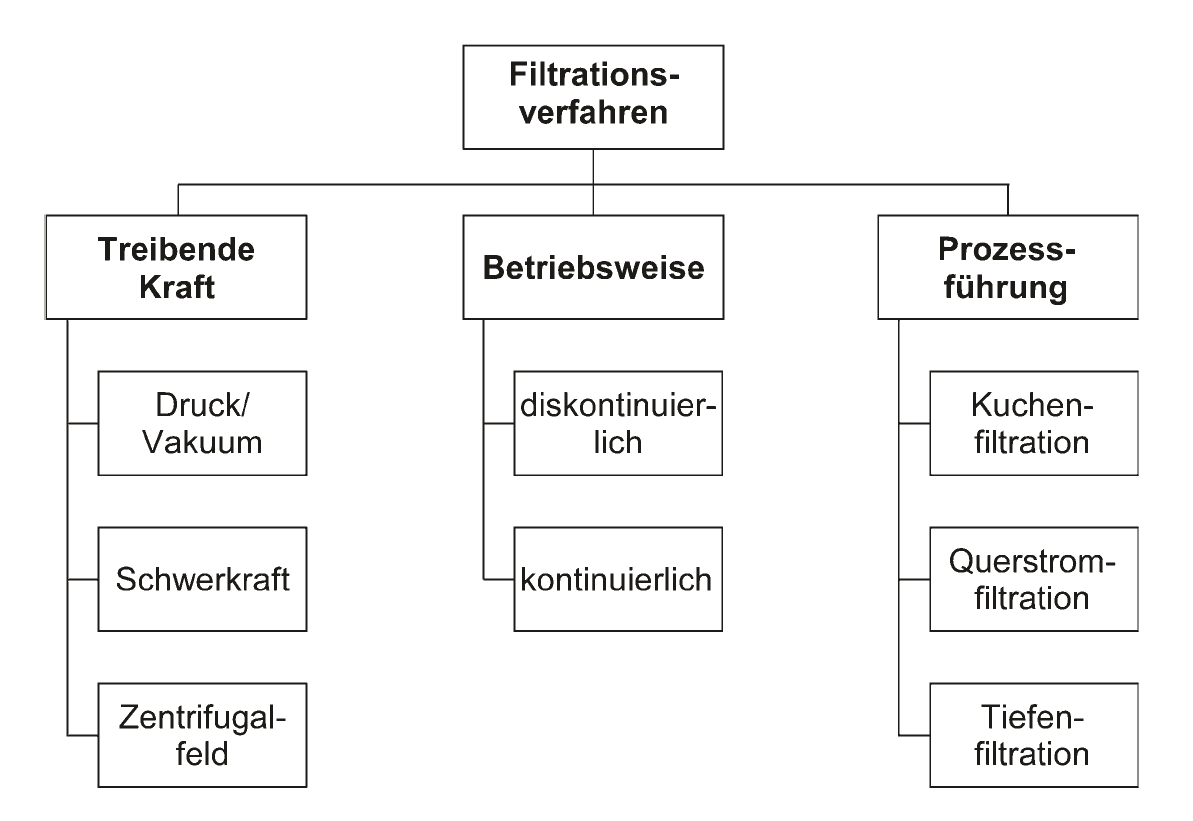
\includegraphics[width=0.8\linewidth]{images/klassifikation_filtrationsverfahren.png}
        \caption[Klassifikation Filtrationsprozesse]{Klassifikation der Filtrationsverfahren nach Kraume \cite{transportvorgänge} }
        \label{fi:klassifikation_filtration}
    \end{center}
\end{figure}
\subsection{Filterparameter}
Da die Abstände einzelner Filterfasern um ein vielfaches größer als die Partikeldurchmesser sind, liegt der modellhaften Beschreibung in der Regel eine einzelne Filterfaser zugrunde.
Wichtigste Kenngröße für die Wirksamkeit eines Filters ist der \ac{eta}.  Dieser wird definiert als das Verhältnis der \ac{con} oder \ac{conM} des zu trennenden Stoffes an der Rohgasseite $c_0$ und der Reingasseite $c_1$.\cite{Staubabscheidung}
\[
\ac{eta} = \frac{c_0 - c_1}{c_0}
\]
In Bezug auf typische Angaben bei der Definition von Partikeln in Medien wäre hier die Verwendung der Mengenkonzentration zu erwarten, es wird jedoch in der Regel die Massenkonzentration verwendet. Mit Hinzunahme der Staubspeicherfähigkeit, welche die Fähigkeit des Filters beschreibt eine bestimmte Masse an Staub zu speichern, ensteht somit eine Grundlage für die Berechnung der Standzeit von Filtern bei der Auslegung der Anlage.
Die Staubspeicherfähigkeit ist hierbei abhängig von der Art des Staubes und einer vorgegebenen Druckdifferenz $\Delta p$, bis zu der der Wert für die Staubmasse gilt, und wird allgemein in Gramm angegeben. \cite{vdi3677_2} \newline
Während der Abscheidegrad \ac{eta} nur eine Aussage über die gesamte abgeschiedene Staubmenge ist, liefert der \ac{etaX} den Abscheidegrad von bestimmten Stäuben. \ensuremath{\bar x} ist hierbei der mittlere Teilchendurchmesser einer bestimmten Staubfraktion. Die Berechnung erfolgt analog zu \ac{eta}. \cite{immission} Unterschiedliche Abscheideprozesse und Filterelemente haben auch unterschiedliche Fraktionsabscheidegrade, und werden entsprechend je nach Anwendungsfall eingesetzt (s. Abb. \ref{fi:frak_filter}).
\begin{figure}[H]
    \begin{center}
        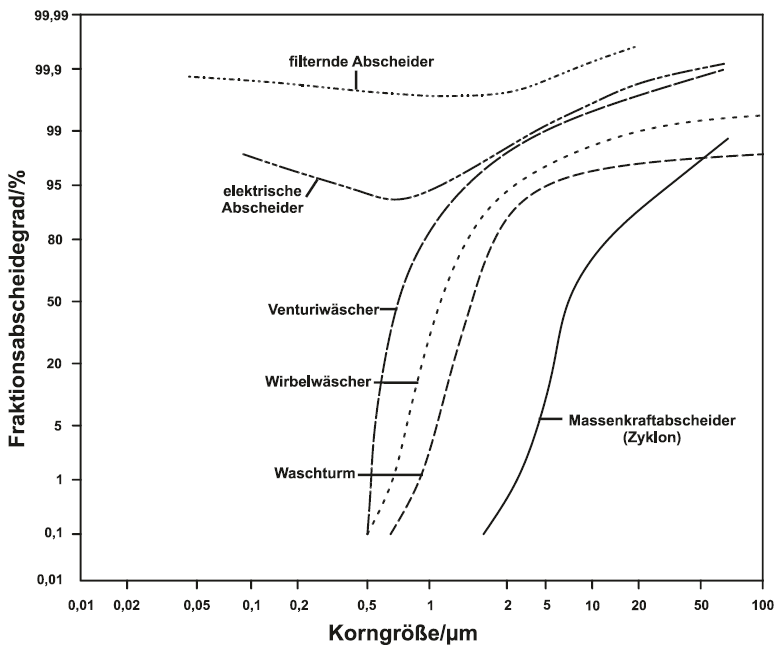
\includegraphics[width=\linewidth]{images/frak_filter.png}
        \caption[Fraktionsabscheidegrad verschiedener Abscheidesysteme]{Fraktionsabscheidegrad verschiedener Abscheidesysteme \cite{frak_filter} }
        \label{fi:frak_filter}
    \end{center}
\end{figure}
\subsection{Überblick über Filterbauarten}
\label{sec:filterbauarten}
Folgend soll ein Überblick über die unterschiedlichen mechanischen Filterbauarten geschaffen werden. Hierbei wird zuerst nur grob zwischen prinzipiellen Bauarten unterschieden, während folgend näher auf die für die Arbeit relevanten Filterbauarten zur Gebäudeklimatisierung und -belüftung eingegangen wird.
\newline
Massenkraftabscheider (Zyklone s. Abb. \ref{fi:zyklon}) zeichnen sich durch einen einfachen Aufbau und geringe Kosten aus. Sie sind besonders für die Abscheidung von Partikeln mit relativ großem mittleren Durchmesser (Grobstäube) geeignet, weswegen ihr Haupteinsatzgebiet die Vorentstaubung von Gasen ist (s. Verlauf \ref{fi:frak_filter}). Bei diesem Wirkpinzip wird die einströmende Luft in eine Kreisbewegung gezwungen, wodurch sich die Staubpartikel in Folge der Zentrifuglkraft an der Zyklonwand niederschlagen. Das Prinzip wird auch bei der Abreinigung von Flüssigkeiten eingesetzt, und wird auf Grund der hohen Betriebssicherheit und geringen Kosten in vielen Industriezweigen eingesetzt.\cite{immission} \newline
Nassabscheider, wie der Venturiwäscher (s. Abb. \ref{fi:venturi}), werden eingesetzt um staub- und gasförmige Schadstoffe abzuscheiden. Wegen der vergleichsweise hohen Betriebskosten werden sie vornehmlich bei kleinen Volumenströmen eingesetzt. Dies ist bedingt durch die Verlagerung des Schadstoffes vom Gas in die genutzte Flüssigkeit (meist Wasser), was eine aufwendige Nachbehandlung erforderlich macht. Entscheidend für die Abscheideleistung ist die Maximierung der Grenzfläche zwischen Tröpfchen und Gas, sowie die Relativgeschwindigkeit der Phasen zueinander. Der Venturiwäscher zählt deshalb zu den sog. Hochleistungswäschern, weil durch die hohen Relativgeschwindigkeiten eine gute Abscheideleistung erreicht wird. Nassabscheider haben jedoch den gemeinsamen Nachteil, dass ein hoher Druckwiderstand an Düse oder Diffusor entsteht, um eine gute Zerstäubung der Waschflüssigkeit zu erreichen. Das heißt, um eine effektive Reinigung zu gewährleisten, muss die Fördereinrichtung für Gas bzw. Flüssigkeit eine entsprechende Leistung erbringen. \cite{immission} \newline
Elektroabscheider (s. Abb. \ref{fi:elektroabscheider}) werden zur Abreinigung großer Volumenströme bei höheren Temperaturen, z.B. in Kraftwerken und Hütten eingesetzt. Die Schadstoffpartikel werden dabei elektrisch aufgeladen, und an einer Niederschlagselektrode abgeschieden. \cite{immission} Über eine Gleichspannung von 30-100 kV werden Elektronen von einer Sprühelektrode aus stark beschleunigt. In Folge werden Gasmoleküle ionisiert, welche wiederum die Staubpartikel negativ aufladen und an die Abscheidewand bzw. Niederschlagselektrode mitreissen. \cite{immission}Hierdurch bildet sich eine Staubschicht an der Niederschlagselektrode, welche als Isolator wirkt, und deshalb periodisch wieder abgetragen werden muss. \newline
Filter besitzen von allen Abscheideverfahren fast unabhängig vom Korndurchmesser die höchsten Abscheidegrade. Nachteil ist, insbesondere bei Tiefenfiltern, die geringe Speicherkapazität, was ihre Einsatzmöglichkeiten einschränkt. Bezeichnend ist die Vielzahl unterschiedlicher Bauformen und Filterwerkstoffe (s. Abb. \ref{fi:filterelemente}). Sie werden allgemein zwischen Oberflächen- und Tiefenfiltern unterschieden (s. Abb. \ref{fi:tiefen_oberfläch}). Bei Oberflächenfiltern bildet sich an der Rohgasseite ein Filterkuchen, welcher selbst als Filter wirkt. Die Zusetzung beider Filtergruppen hat einen zunehmenden Druckverlust am Filter zur Folge, und ist eine wichtige und betriebsrelevante Größe (s. Abb. \ref{fi:druckverlust_abr}). Der Filterkuchen wird periodisch wieder abgetragen. Hierbei werden Vibrationen/Rütteln, oder auch Druckimpulse/Pneumatik eingesetzt. Häufigstes Verfahren hierfür ist ein Gegenspülen im Online-Betrieb mittels Klappensteuerungen in den Rohrelementen.\cite{Staubabscheidung} Ziel ist die Regeneration des Filters, allerdings tritt immer eine gewisse Tiefenfiltration, und folglich Verschleiß auf, wodurch die Filterelemente getauscht werden müssen. Filter gehören zu den ältesten Abscheideverfahren, ihrer geringen chemischen- und Temperaturbeständigkeit konnte mit modernen Werkstoffen entgegengewirkt werden, wobei heute Glas- und Mineralfasern sowie diverse Kunstfasern wie Aramid bis Stahlfasern eingesetzt werden. Die Abbildung \ref{fi:filterelemente} verdeutlicht hierbei die Vielseitigkeit der unterschiedlichen Filterbauarten, deren häufigste Vertreter Schlauch- und Taschenfilter sind. \cite{immission}
\begin{figure}[ht!]
    \begin{center}
%
       \subfigure[Zyklon]{%
           \label{fi:zyklon}
           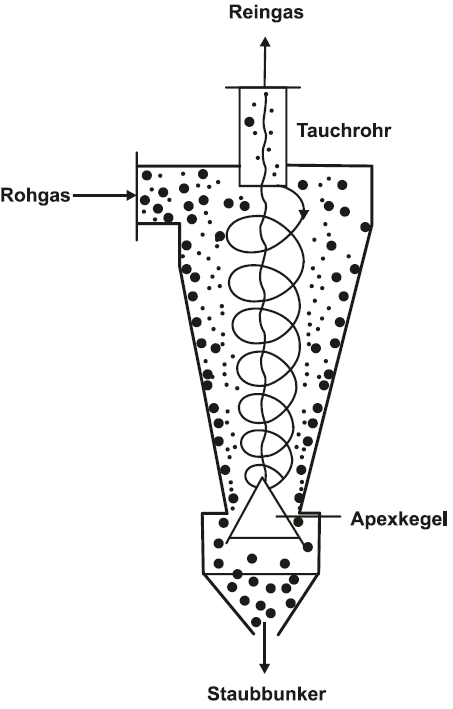
\includegraphics[width=0.5\textwidth]{images/zyklon.png}
       }%
       \subfigure[Venturiwäscher]{%
          \label{fi:venturi}
          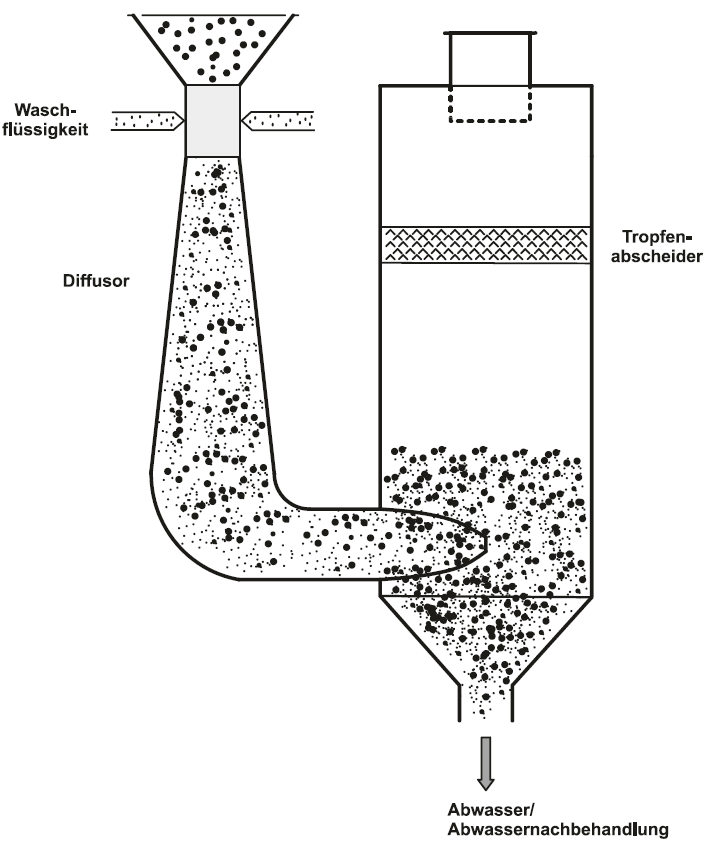
\includegraphics[width=0.5\textwidth]{images/venturi.png}
       }\\ %  ------- End of the first row ----------------------%
       \subfigure[Elektroabscheider]{%
           \label{fi:elektroabscheider}
           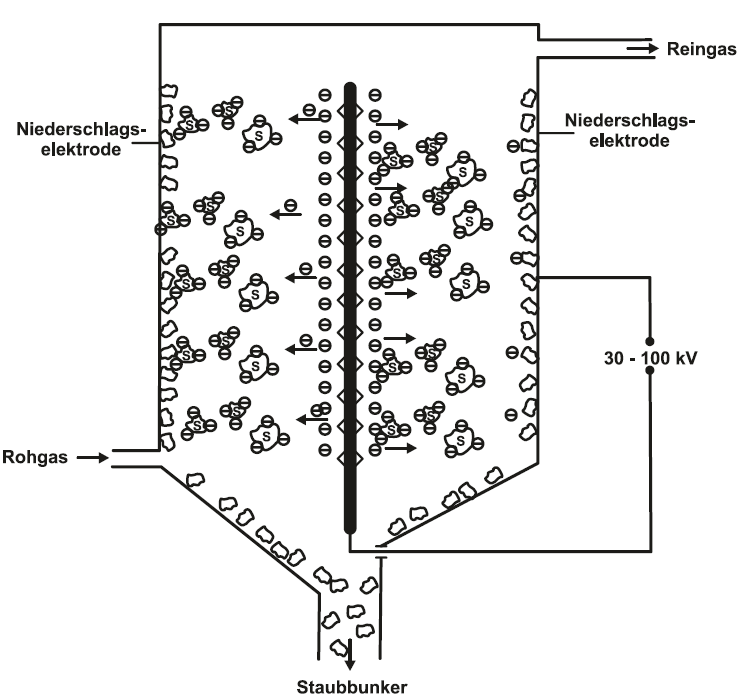
\includegraphics[width=0.5\textwidth]{images/elektro.png}
       }%
       \subfigure[Filterelemente]{%
           \label{fi:filterelemente}
           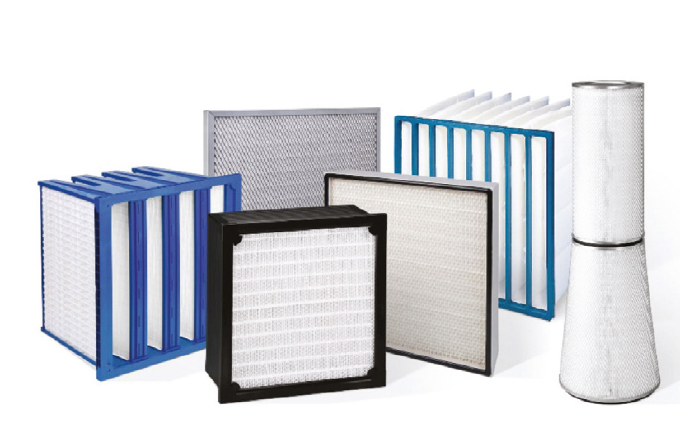
\includegraphics[width=0.5\textwidth]{images/filterelemente.png}
       }\\%
%
   \end{center}
   \caption{%
       Unterschiedliche Verfahrensprinzipien zur Staub- und Aerosolabscheidung; Quellen: \ref{fi:zyklon} - \cite{zyklon}; \ref{fi:venturi} - \cite{venturi}; \ref{fi:elektroabscheider} - \cite{immission}; \ref{fi:filterelemente} - \cite{filterelemente}
    }%
  \label{fig:verfahren}
\end{figure}
\newpage
\subsection{Filtereffekte}
\label{sec:filtereffekte}
Bei der Abscheidung von Partikeln aus Medien wirken unterschiedliche Filtereffekte. Diese Effekte treten je nach Größe (Durchmesser) der Partikel und Filterart unterschiedlich stark auf. Folgend werden diese Effekte kurz dargestellt, wobei die Effekte absteigend mit Hinblick auf die Stärke des Effekts bei kleiner werdender Partikelgröße geordnet sind. Bei einer detaillierten Untersuchung mit variiertem Volumenstrom können sich die Anteile der wirkenden Effekte deutlich verschieben, was signifikanten Einfluss auf die Filterleistung hat.
\begin{figure}[H]
    \begin{center}
        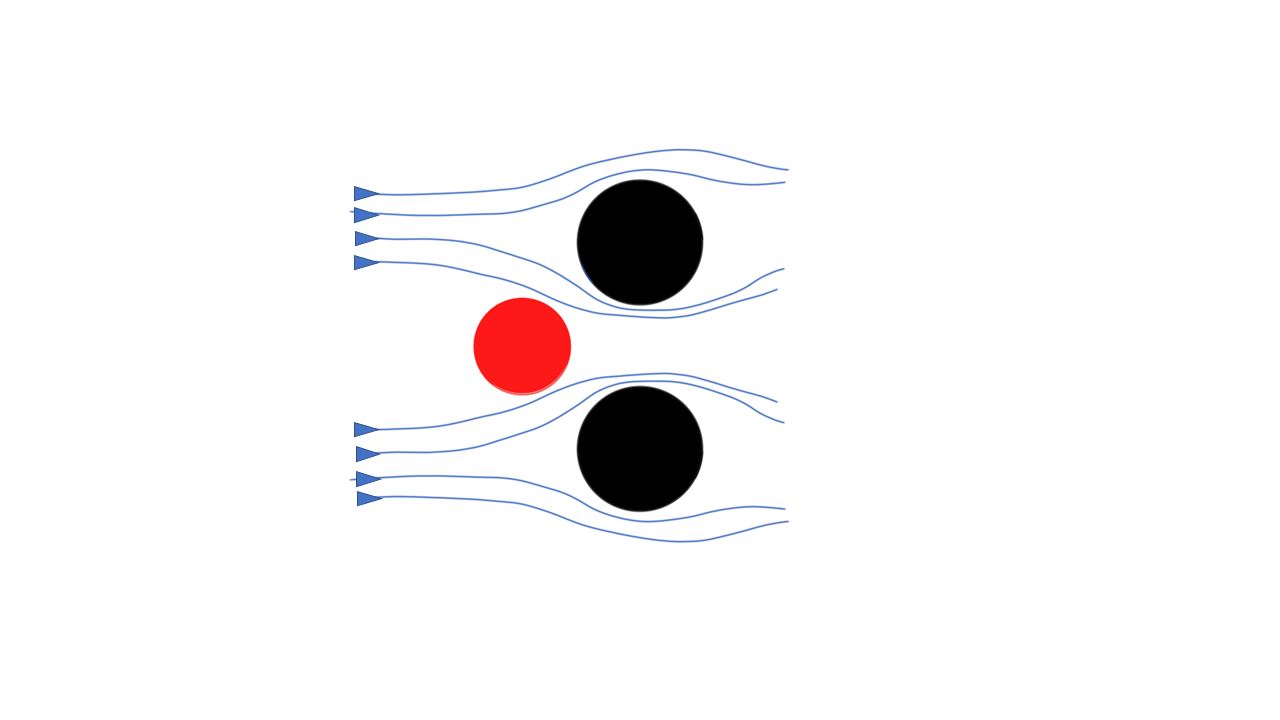
\includegraphics[width=\linewidth]{images/sieb2.png}
        \caption[Siebwirkung]{Prinzipskizze Siebwirkung}
        \label{fi:siebwirkung}
    \end{center}
\end{figure}
Wenn der Durchmesser der Partikel größer ist als der Abstand der Filterfasern zueinander, kann der Partikel das Filtermaterial nicht durchdringen. (siehe Abb. \ref{fi:siebwirkung}) Folglich tritt der Effekt verstärkt mit zunehmender Strömungsgeschwindigkeit und Größe bzw. Masse der Partikel auf. Der Siebeffekt ist im Fall von Tiefenfiltern bei der Beurteilung der Abscheidung quasi irrelevant, denn die Porosität der genutzten Filtermedien liegt bei bis zu 99,8 \% , folglich liegen die Fasern um ein vielfaches weiter auseinander, als der Durchmesser der abgeschiedenen Partikel. \cite{vdi3677_2} Bei Oberflächenfiltern wird der Siebeffekt, zumindest in der VDI Richtlinie 3677 - Blatt 1 "Filternde Abscheider - Oberflächenfilter" \cite{vdi3677_1}, nicht explizit als relevanter Effekt aufgeführt. 
\begin{figure}[ht!]
    \begin{center}
%
       \subfigure[Trägheitseffekt]{%
           \label{fi:traegheit}
           \includegraphics[width=0.5\textwidth]{images/trägheit.png}
       }%
       \subfigure[Sperreffekt]{%
          \label{fi:sperrefekt}
          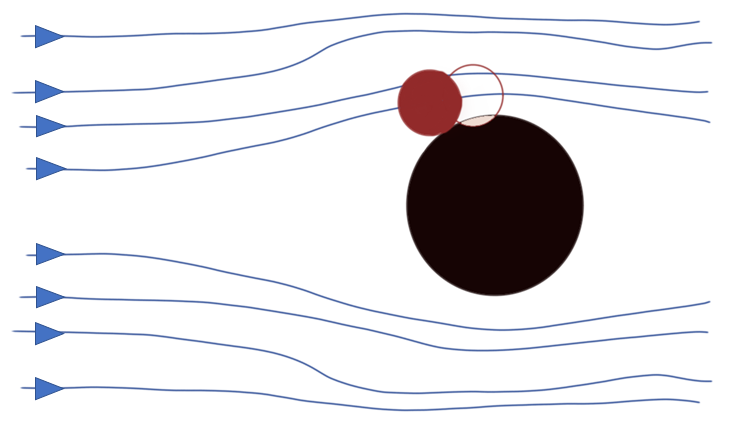
\includegraphics[width=0.5\textwidth]{images/sperr.png}
       }\\ %  ------- End of the first row ----------------------%
       \subfigure[Diffusionseffekt]{%
           \label{fi:diffusion}
           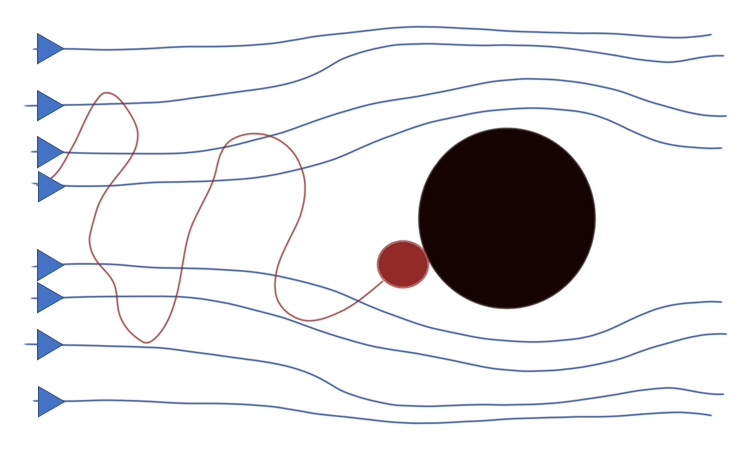
\includegraphics[width=0.5\textwidth]{images/diffusion2.png}
       }%
       \subfigure[Elektrostatische Anziehung]{%
           \label{fi:elektrostatisch}
           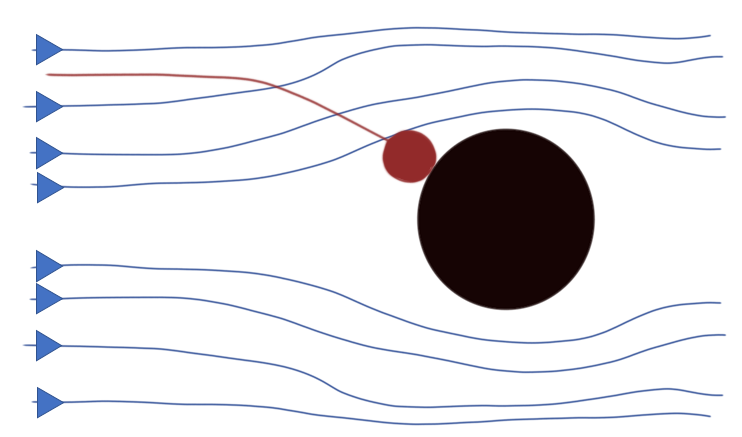
\includegraphics[width=0.5\textwidth]{images/elektrostatisch1.png}
       }\\%

%
   \end{center}
   \caption{%
       Prinzipskizzen von Filtereffekten, welche bei der Partikelabscheidung mit Faserfiltern auftreten
    }%
  \label{fig:filtereffekte}
\end{figure}
Relativ große, oder schwere, Partikel sind auf Grund ihrer Masse zu träge um dem Luftstrom um die Filterfaser zu folgen (siehe Abb. \ref{fi:traegheit}). Dadurch kommen sie mit der Faser in Berührung und bleiben dort hängen. 
Leichtere Partikel folgen hingegen der Strömung um die Faser. Genauer folgt der Masseschwerpunkt des Partikels der Strömung um die Faser. Wenn der Abstand dieses Punktes zur Faser den Abstand des Punktes zur Außenkontur des Partikels unterschreitet, bleibt der Partikel durch Adhäsionskräfte haften. Dieser Vorgang wird als Sperreffekt bezeichnet (siehe Abb. \ref{fi:sperrefekt}). Hierbei begünstigen große Partikeldurchmesser im Verhältnis zum Faserdurchmesser die Wahrscheinlichkeit eines Auftreffens auf die Faser. Der Effekt wird mathematisch mit dem \ac{R} in Abhängigkeit der \ac{d} von Faser~$\ac{d}_{F}$ und Partikel~$\ac{d}_{P}$ beschrieben. \cite{vdi3677_2} 
\[
R = \frac{d_P}{d_F}
\]

Der Sperreffekt ist insbesondere bei Oberflächenfiltern mit Filterkuchen der primäre Abscheidemechanismus. \cite{vdi3677_2} 
Bei kleinen Durchmessern ( \ac{d} kleiner 1 \si{\micro\metre} \cite{Grundlagen_Filtertechnik} bzw. kleiner 0,5 \si{\micro\metre} \cite{vdi3677_2} )folgen die Partikel nicht mehr allein der Strömung. Geringe \ac{u} von \ac{u} $<$ 0,1 \si{\metre\per\second} begünstigen ebenfalls den sog. Diffusionseffekt (s. Abb. \ref{fi:diffusion}).
Es treten auch Transportmechanismen durch elektrostatische Kräfte zwischen Partikeln und Filtermedium auf (s. Abb. \ref{fi:elektrostatisch}). Diese treten auf, wenn Partikel bzw. Filtermedium elektrostatisch aufgelagen sind, was in manchen Filtern gezielt herbeigeführt wird \cite{vdi3677_2}. Die Abschätzung des Einflusses, und das Design solcher Filter ist eher speziell, und basiert auf Approximationsgleichungen (s. auch \cite{faser_elektro}).
\subsection{Filterklassen Luftfilter}
\label{sec:filterklassen}
Um schädliche Effekte auf Umwelt und Menschen abzuwenden, müssen Filter in der Lage sein unterschiedliche Aerosole herauszufiltern. Diese Aerosole können z.B. in der Luft schwebende Metallfragmente, Faserreste, sowie Organsimen wie Pilzsporen, Pollen und Keime sein. Für die Gesundheit ist neben dem Schadstoffgehalt bzw. Toxizität der Partikel die Größe der Staubpartikel der entscheidende Parameter. \cite{Grundlagen_Filtertechnik} Partikel mit einem Durchmesser größer als 10 µm werden als Grobstaub bezeichnet. Dieser Grobstaub bleibt in den Härchen und Schleimhäuten des Nasen-Rachenraums hängen. Kleinere und kleinste Staubpartikel, sog. Feinstaub können diese natürlichen Filter durchdringen, und werden daher als inhalierbar bzw. alveolengängig bezeichnet. \newline
Basierend auf dieser Unterscheidung werden ebenso die eingesetzten Filterklassen zwischen Grobstaubfilter und Feinstaubfilter unterschieden. Bei noch kleineren zu filternden Partikelgrößen, beispielsweise bei Reinraumanwendungen kommen sog. Schwebstofffilter zum Einsatz. Diese unterscheiden sich jedoch in Hinblick auf die Anteile der wirkenden Filtereffekte von den anderen beiden beschriebenen Filterarten. \newline
Staubfilterklassen werden eigentlich seit Mitte 2018 nicht mehr nach EN 779 klassifiziert (s. Abb. \ref{fi:filter_gmf}), die veralteten Klassen finden aber noch Verwendung in Asien, und werden auch immernoch in z.B. Produktkatalogen von Filterherstellern angegeben. Auf die Prüfverfahren soll hier nicht im Detail eingegangen werden, es ist für das Verständnis der Arbeit jedoch wichtig zu bedenken, das auch der sog. synthetische Staub (ASHRAE-Staub), wie auch der Staub mit durchschnittlichen Partikeldurchmessern von 0,4 µm, selbst genormt ist (Prüfstaub). Im Rahmen der Vergleichbarkeit unterschiedlicher Filter ist dies unvermeidbar, entsprechend kann eine Prüfung aber niemals die Realität abbilden, da die Staubzusammensetzung ein variabler Eingangswert ist. Die Geltungsbereiche der Abscheidegrade sind außerdem nur bis zu einer definierten Enddruckdifferenz garantiert bzw. geprüft. Die Mindesteffizienz bezeichnet den mindestens erreichten Abscheidegrad des schlechtesten Prüfergebnisses eines Filters aus einer Prüfreihe. Grobstaubfilter werden bei der Prüfung nicht mit 0,4 µm Staub beaufschlagt.\cite{Grundlagen_Filtertechnik}
\begin{figure}[H]
    \begin{center}
        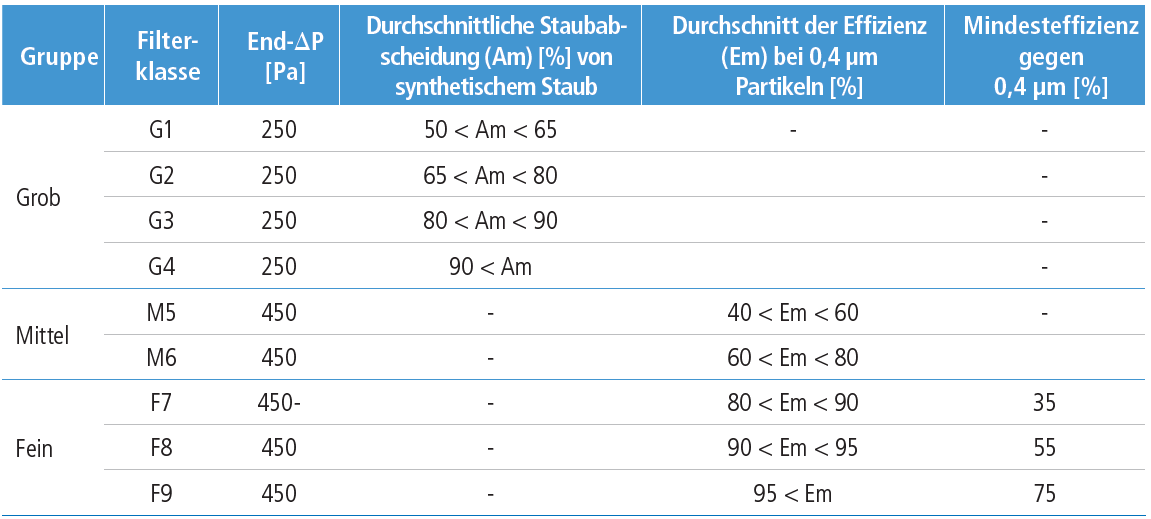
\includegraphics[width=\linewidth]{images/filter_GMF.png}
        \caption[Filterklassen]{Filterklassen Grob, Mittel, Fein nach EN 779}
        \label{fi:filter_gmf}
    \end{center}
\end{figure}
Mit neuen Erkennnissen über die Schädlichkeit von Feinstaub für die Gesundheit wurde eine Neuerung der Normen zur Klassifizierung von Filtern angestoßen. Diese Entwicklungen mündeten in einer neuen Norm ISO 16890 \cite{16890}. Da die reale Verteilung der Partikelgrößen nicht den festen 0,4 µm nach EN 779 entspricht, ist diese Prüfung realitätsnäher. Die neue Gruppierung ePMx beschreibt dabei die gesamte Staubfraktion von 0,3 µm bis x µm (s. Abb. \ref{fi:epmX}). Coarse beschreibt hierbei Filter, die für Partikelgrößen von 0,3 - 10 µm einen Abscheidegrad von 50 \% unterschreiten. Zusätzlich wird eine Angabe über den Durchschnitt zwischen Anfangs- und Mindest-Abscheidegrad bei der Prüfung gemacht, wobei  auf 5\%-Schritte gerundet wird. Beispielsweise beschreibt ein Filter ISO ePM10 85\% einen Filter, der im Bereich PM10 (0,3 - 10 µm) einen Abscheidegrad von 85 - 90\% erreicht.
\begin{figure}[H]
    \begin{center}
        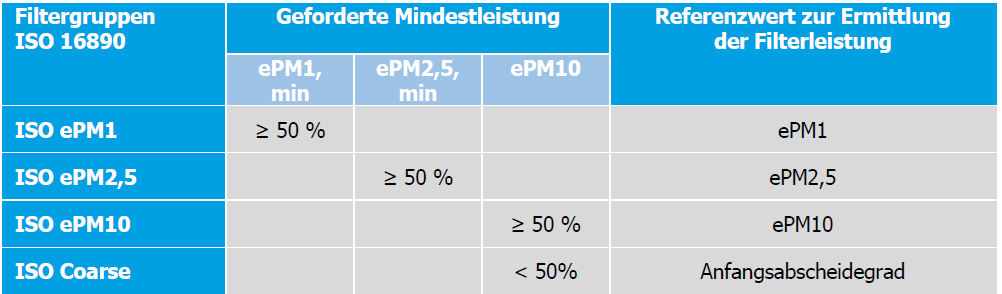
\includegraphics[width=\linewidth]{images/epmX.png}
        \caption[Filtergruppen ISO 16890]{Einteilung der Filtergruppen nach ISO 16890 \cite{altneu}, \cite{16890}}
        \label{fi:epmX}
    \end{center}
\end{figure}
Für Stäube im Sub-µm Bereich werden Schwebstofffilter eingesetzt. Diese Filter liefern die höchsten Abscheidegrade der mechanischen Luftfiltration, und werden primär als finale Filterstufe bei hochsensiblen Prozessen, wie OP-Räumen, Reinräumen und militärischen Anwendungen eingesetzt. Desweiteren werden Schwebstofffilter zur sicherheitsrelevanten Abluftbehandlung, z.B. bei der Asbestsanierung oder Nuklearindustrie, eingesetzt. \newline 
Schwebstofffilter sind dabei in der Lage extrem kleine Partikelgrößen, wie Viren, Bakterien und nanoskopische Stäube abzuscheiden. Relevante Normen sind hierbei EN 1822 \cite{1822} und ISO 29463, sie sind daher entkoppelt von der Neuerung bei den anderen Staubfiltern.
Die Qualitätsansprüche an Prüfung, Produktion und Installation solcher Filter sind entsprechend hoch. Hierfür wird zunächst mit dispersen Prüfaerosolen die \ac{MPPS} bestimmt, und der Filter anschließend anhand dieser geprüft. Während bei \ac{epa}-Filtern nur Abscheide- und Durchlassgrad des gesamten Filters geprüft werden, erfolgt bei \ac{hepa} und \ac{ulpa} Filtern zusätzlich eine Prüfung auf Leckagen. Die Filtermedien sind meist empfindlich gegenüber mechanischen Belastungen. \cite{Grundlagen_Filtertechnik} Bei der Produktion auftretende Toleranzschwankungen und kleinste Verklebefehler führen zu lokal stark erhöhten Partikeldurchlässen. Bei diesem Prüfschritt wird mit Prüfnebel und optischen Verfahren zunächst die schwächste Stelle(n) des Filters ermittelt, und diese anschließend gezielt mit dem \ac{MPPS}-Staub geprüft (Gruppierungen s. Abb. \ref{fi:filter_ehu}).
\begin{figure}[H]
    \begin{center}
        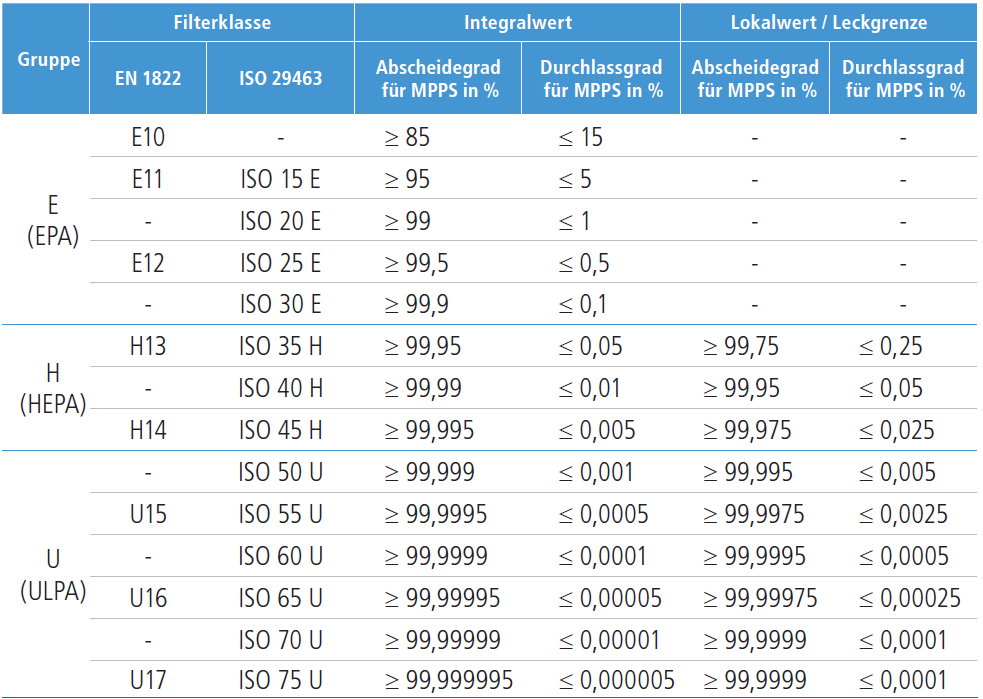
\includegraphics[width=\linewidth]{images/filter_EHU.png}
        \caption[Filterklassen Schwebstoffe]{Schwebstofffilterklassen EPA, HEPA, ULPA nach DIN EN 1822 \cite{1822}}
        \label{fi:filter_ehu}
    \end{center}
\end{figure}
\subsection{Aufbau von Raumlufttechnischen Anlagen}
\label{sec:aufbau}
Der Aufbau von Raumlufttechnischen Anlagen ist so vielfältig wie die Einsatzzwecke der ausgerüsteten Gebäude. Eine Vorstellung sämtlicher zu berücksichtigenden Eigenschaften bei der Planung solcher Anlagen würde zu viel Raum in dieser Arbeit fordern. Stattdessen wird folgend auf die für die Arbeit relevanten Aspekte solcher Anlagen eingegangen. \newline
Grundlegendes Entscheidungsmerkmal von Raumlufttechnischen Anlagen nach Bohne \cite{tavg} ist die Unterscheidung zwischen Anlagen mit Lüftungsfunktion und solchen ohne Lüftungsfunktion. Im Rahmen dieser Arbeit ist eine Lüftungsfunktion Vorraussetzung für die Sinnhaftigkeit einer Filterüberwachung.
Anlagen können zusätzlich, unabhängig von der Lüftungsfunktion, folgende Aufgaben erfüllen:
\begin{itemize}
    \item H - Heizen
    \item K - Kühlen
    \item B - Befeuchten
    \item E - Entfeuchten
\end{itemize}
Eine Anlage, die nur Luft transportiert (und ggf. filtert), wird Lüftungsanlage genannt. Wird keine Außenluft zugeführt handelt es sich um eine Umluftanlage. Diese Definition umfasst ebenfalls Anlagen, die maximal eine der genannten Behandlungsfunktionen erfüllen. Werden zwei oder drei Teilfunktionen erfüllt wird die Anlage als Teilklimaanlage, respektive Umluftteilklimaanlage bezeichnet.
Nur wenn alle Teilfunktionen erfüllt werden handelt es sich um eine (Umluft-)Klimaanlage. \newline
Weitere Unterscheidungen erfolgen dann auf Grundlage des genutzten Mediums zum Temperaturmanagement bswp. Wasser, Kühlmittel.\cite{tavg}
Im Kontext der Fragestellung hochinterssant ist die Grundkategorie der Regelung oder Steuerung (s. Abb. \ref{fi:regelungsarten}), sowie die hierbei auftretender Besonderheiten, die einen denkbaren Einfluss auf den Filterverschleiß haben können.
\begin{figure}[H]
    \begin{center}
        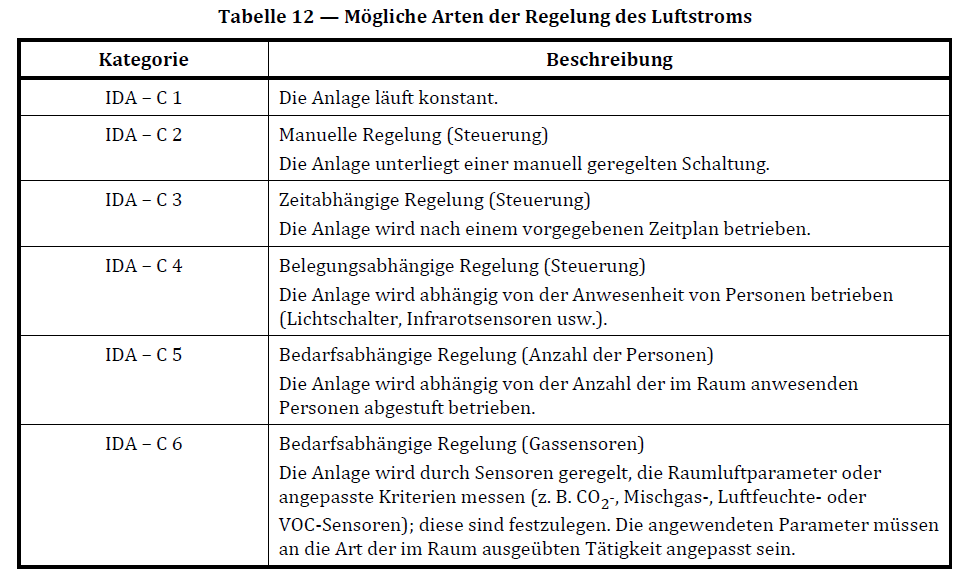
\includegraphics[width=\linewidth]{images/arten_regelung.png}
        \caption[Regelungsarten Luftstrom]{Grundkategorien Regelung aus DIN EN 16798-3 \cite{16798} }
        \label{fi:regelungsarten}
    \end{center}
\end{figure}
Es ist ebenfalls relevant, ob die Regelung für einzelne Räume oder zentralisiert für Gebäudebereiche realisiert wird. Unabhängig hiervon ist für die Belastung der Filter der Volumenstrom von zentraler Bedeutung. Bei den Klassen IDA-C4 und niedriger wird ein fester Sollwert für den Volumenstrom bei der Auslegung festgelegt. Das heißt im Sinne einer Überwachung des Filerverschleißen ist hier prinzipiell nur die Betriebsdauer zu erfassen. Bei den Klassen IDA-C5 und C6 wird dieser Sollwert jedoch bedarfsorientiert angepasst, und muss somit als zusätzliche zeitvariante Variable in das Modell zur Vorhersage einfließen. Die Norm weißt in diesem Fall auf Druckschwankungen hin, welche durch den variierbaren Luftvolumenstrom verursacht werden können. \cite{16798} Diese müssten im Rahmen von Messungen unter Betriebsbedingungen erfasst werden, da sie von den örtlichen Gegebenheiten wie z.B. Windstärke und Anlagenmerkmalen abhängig sind. \newline
Bei Grobstaubfiltern ist in der Regel außerdem der Nennvolumenstrom bzw. Anströmgeschwindikeit einzuhalten, während bei Feinstaub- und Schwebstofffiltern je nach Bauform Abweichungen von +20\% bis -90\% zulässig sind.\cite{Grundlagen_Filtertechnik} Dies ist durch die wirkenden Filtereffekte bei Grobstaubfiltern bedingt, die stark von der Strömungsgeschwindigkeit abhängig sind (s. Kap. \ref{sec:filtereffekte}).
Der Fokus dieser Arbeit liegt auf dem Konzept bzw. der Machbarkeit. In diesem Rahmen wird der Volumenstrom als belegungsgesteuert angenommen, Einzelheiten der Anlagengestaltung vereinfacht, und eine Volumenstromregelung zur Verhinderung von Druckschwankungen im System vorausgesetzt. Weitere Anforderungen an eine solche Anlage zur Realisierung einer prädiktiven Überwachung ergeben sich aus den folgenden Unterkapiteln, und umfassen Möglichkeiten zur digitalen Datenerfassung, Netzwerkfähigkeit (Nutzung von Bussystemen), sowie Rechenkapazitäten.
\section{Grundlagen IIoT}\label{sec:iiot}
Das \ac{iiot} ist die Adaption des \ac{iot} auf die industrielle Produktionslandschaft. Die Grenzen zwischen den Begriffen \ac{cps}, \ac{iot} und \ac{i40} sind dabei fließend, und somit sinnbildlich für den neuartigen und volatilen Charakter der hintergründigen Technologien.
Grundsätzlich werden hierbei zahlreiche physikalische Objekte, sog. "Things", mit der Fähigkeit ausgestattet Informationen zu übertragen, und als Netzwerk (Internet) miteinander verknüpft. Dabei können die Things selber sowohl als Server als auch als Client agieren. Aufgaben wie z.B. Datenaggregation und -analyse können hierbei von den Things übernommen werden. Digitale Prozesse laufen also nicht mehr zwangsläufig  auf einem einzigen, monolithischen Server(cluster)-System ab, sondern zunehmend dezentralisiert.

"Grundidee [...] ist die Integration und
Vernetzung unterschiedlicher intelligenter Objekte in einem Produktionsumfeld. [...], dass mithilfe von Cloud Computing und analytischen
Auswerteverfahren, die wesentlichen Informationsbausteine
gewonnen werden können, die zu
effizienteren Serviceprozessen und zu einem optimierten
Kosten-Nutzenverhältnis führen. Für
Maschinen- und Anlagenbauer kommt heute die
Kombination von Produkt und Dienstleistung
im Sinne eines Product Service Systems immer
stärker in den Fokus." \cite{i40_instandhaltung}

Hierbei stellt die Integration eines Sensornetzwerkes in das Produktionsumfeld, mit dem Ziel einen Datenstrom zu erzeugen, die Grundlage. Ausgehend von diesem Datenstrom kann das Unternehmen kontinuierlich und in Echtzeit Informationen über seine physikalischen und virtuellen Bestandteile sammeln.
\ac{iiot} meint somit einen Bestandteil eines Szenarios, bei dem, innerhalb einer Cloud-Infrastruktur, z.B. automatisierte Funktionen zur Datenanalyse eingebunden werden. Hierdurch werden neue Nutzenpotenziale für das Unternehmen erschlossen. \cite{i40_instandhaltung}
Ein Beispiel hierfür wäre das Abrufen von Produktionsmessdaten vor der Bestellung durch den Kunden in einem Webshop. Der Kunde kann im Prusa Onlineshop für Filamente für \ac{fdm} 3D-Drucker während der Bestellung die Messdaten des Filamentdurchmessers, welcher einer der entscheidenden Faktoren für eine hohe Druckqualität ist, aus der Produktion abrufen (siehe Abb. \ref{fi:prusa}). Dies steigert das Kundenvertrauen in die Produktqualität, was wiederum einen erhöhten Umsatz für das Unternehmen generiert.
\begin{figure}[H]
    \begin{center}
        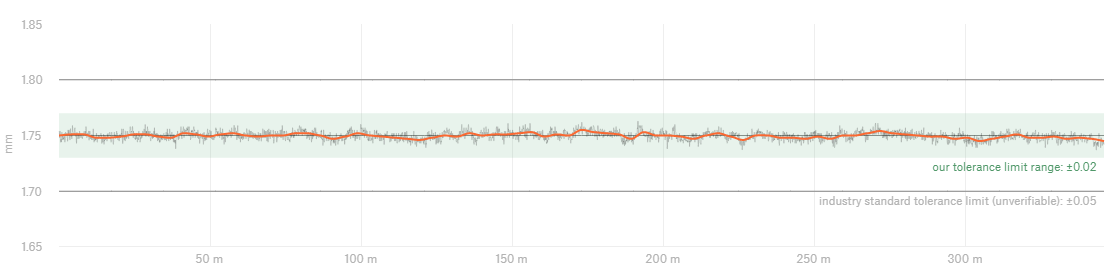
\includegraphics[width=\linewidth]{images/prusa.png}
        \caption[Prusament]{Prusa PLA Filament 1.75mm \cite*{prusa} }
        \label{fi:prusa}
    \end{center}
\end{figure}
Nicht zu unterschätzen ist hierbei in der Realität allerdings der Integrationsaufwand, welcher weit über den Aufbau eines Sensornetzwerkes mit eventueller Datenbank hinausgeht. Um ein solches System auch gewinnbringend einzusetzen ist es nötig \ac{api}'s für diverse Backendservices bereitzustellen. Desweiteren müssen diese Services auch anwendungsorientiert entwickelt bzw. programmiert werden, und schlussendlich auch in interne Systeme, wie z.B. \ac{erp} und \ac{bi} integriert zu werden.
Ein noch weiter gehender Schritt ist in diesem Zuge eine Schnittstelle zu den Systemen externer Dienstleister herzustellen, bspw. zur schnelleren Abwicklung von Wartungsaufträgen für Produktionsanlagen. Dies erfordert einheitliche Übertragungsstandards, und wird durch einander ähnliche Datenmodelle erleichtert.
\subsection{Architektur von IIoT Netzwerken}
Sollen die physischen Objekte im digitalen System lediglich repräsentiert werden, reicht eine Identifikation mittels \ac{qr} oder \ac{rfid} aus. Ein zentrales System kann nun die gekennzeichneten Objekte verfolgen und dem Nutzer relevante und aufbereitete Daten zur Verfügung stellen.
Sollen die Objekte selbst jedoch Daten verarbeiten, zum Beispiel ein Mikrocontroller der ein Sensorcluster ausliest und versorgt, benötigt dieser eigene Rechenkapazitäten, eine Datenschnittstelle bzw. Netzwerkanbindung und eine Energieversorgung, um Sensorwerte auszulesen, zu verarbeiten und für das System bereitstellen zu können. Diese Argumente machen deutlich, dass eine allgemeingültige Aussage zu der konkreten Architektur von \ac{iiot} Netzwerken nahezu unmöglich ist.
Derartige Netzwerke erfordern jedoch immer Übertragungsstandards, eine entsprechende Infrastruktur zur Datenübertragung, mehr oder weniger dezentralisierte Rechenkapazitäten, sowie Möglichkeiten zur Speicherung von Daten.
\begin{figure}[H]
    \begin{center}
        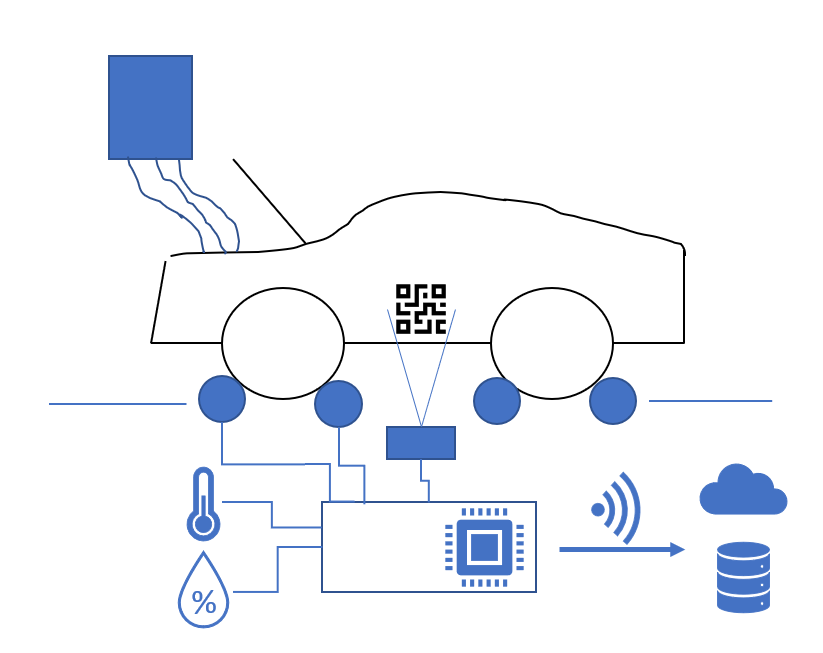
\includegraphics[width=\linewidth]{images/beispiel_iiot.png}
        \caption[Beispiel IIoT]{Auto Teststand mit IIoT Umsetzung}
        \label{fi:auto_iiot}
    \end{center}
\end{figure}
Der Teststand in Abbildung \ref{fi:auto_iiot}) soll heirzu als Beispiel dienen, und erfasst daher innerhalb eines eigenen Netzwerkes mit eigenen Protokollen und eigener Messdatenerfassung Umwelt-, Produkt-, und Testdaten. Die Zelle agiert dabei als autarkes \ac{cps}, und kann dabei Umwelteinflüsse auf Testparameter ausregeln. Ebenso ist es in der Lage die Testanalyse autonom von einem zentralen Server auszuführen, und z.B. Anomalien im Ablauf zu erkennen und zu melden. Die Testdaten werden drahtlos, in aggregierter und verknüpfter Form, an Backendservices für z.B. Produktivitätsdashboards gesendet. Während Rohdaten, wie Zeitreihen, über eine Cloud in spezialisierten Datenbanken hinterlegt werden. \newline Eine solche Architektur hat im Gegensatz zu einer traditionellen, monolithischen Architektur den Vorteil, dass der Datenstrom zu einem einzelnen Server(cluster) reduziert wird. Services für eine nachgelagerte Analyse, wie Prozessoptimierungen, können die Rohdaten je nach Bedarf von den Datenbanken abrufen. Die Testergebnisse müssen nicht von einem zentralen Server für mehrere Zellen parallel generiert werden, sondern werden direkt und aufbereitet an den Webserver für das Dashboard übergeben. Diese verzweigte Netzwerkarchitektur und Verteilung von Berechnungsaufgaben verringert den Netzwerktraffic, vermeidet Bottlenecks (Balancing von Serveranfragen) und berücksichtigt die Einschränkungen bei der Anzahl von Teilnehmern (z.B. Vergabe von IP-Adressen).
Hieraus ergibt sich jedoch der Nachteil des zusätzlich Wartungsaufwands, z.B. bei einem Variantenwechsel des Produkts. Moderne \ac{iot} Cloud Lösungen stellen hierfür Funktionalitäten bereit, um mehrere verknüpfte Things von einem einzigen, virtuellen Ort aus zu aktualisieren bzw. zu programmieren.
\subsection{Protokolle für Sensornetzwerke}
In Anlagen zur Klimatisierung, Belüftung, Heizung etc. von Gebäuden werden viele Sensoren und Stellglieder eingesetzt. Für eine echtzeitfähige Erfassung und Verarbeitung der Messgrößen, sowie Ansteuerung der Stellglieder reicht bei der üblichen Komplexität dieser Systeme eine analoge Datenübertragung über bspw. 5V- oder 10V-Technik nicht mehr aus. Digitale Transportmechanismen haben zudem den Vorteil geringerer Störanfälligkeit und die Fähigkeit Informationen über größere Strecken zu übermitteln. \cite{gebauto}
Um ein solches Kommunikationsnetzwerk bereitstellen zu können, sind sog. Bussysteme erforderlich. Diese ermöglichen eine Einbindung von Mess- und Regelgeräten in ein System. Beispiele hierfür sind Messumformer, Sensoren, Aktoren und Regler. \cite{61158-1} \newline
Auf Feldebene werden die üblichen analogen Datenübertragungen zwar durchaus noch genutzt, darüber hinaus hat die zunehmende Verfügbarkeit und die Verringerung der Kaufpreise von Mikrocontrollern in den 1980ern dazu geführt, dass Feldbus- und Bus-systeme in die \ac{glt} eingeführt wurden (s. Kap. \ref{sec:regelungsart}).
Die hierfür genutzten Protkolle sind über das ISO/OSI Schichtenmodell charakterisiert. Hierbei wird aufbauend auf die physikalische Schicht, welche die Übetragung von Informationen bitweise implementiert, mehrere Schichten mit abnehmenden Abstraktionsgrad der Informationen genutzt. Das hierfür weltweit verbreitete Referenzmodell beinhaltet sieben Schichten. \cite{osi} Diese setzen sich beispielhaft anhand eines Browserfensters wie folgt zusammen:
\begin{itemize}
    \item 7 - Application Layer      -   Browser Bedienelemente
    \item 6 - Presentation Layer     -   HTML-Rendering
    \item 5 - Session Layer          -  Tab-Browsing
    \item 4 - Transport Layer        -   TCP / UDP
    \item 3 - Network Layer          -   IP-Adressen
    \item 2 - Data Link Layer        -   MAC-Adressen
    \item 1 - Physical Layer         -   Digitale Signale
\end{itemize}
Die unterschiedlichen Schichten werden dabei von ebenso unterschiedlichen Hardware- bzw. Softwareschichten implementiert bzw. interpretiert.
Die in \ac{iiot} bzw. in der \ac{glt} genutzten Protokolle nutzen hierfür in der Regel die Schichten 1-4. Da die Daten lediglich in einem \ac{m2m} Szenario genutzt werden, und zudem Echtzeitfähigkeit zur Erfüllung von Regelungsaufgaben im Falle von \ac{ddc} Unterstationen gefordert wird, sind Session-Informationen i.d.R. überflüssig, bzw. führen zu einem inaktzeptablen Overhead.
\section{Grundlagen KI}
\label{sec:grundlagenKI}
Die Grundlagen für selbstlernende Algorithmen wurden bereits in den 50ern gelegt. Seitdem hat vorallem die immer stärker werdende Rechenleistung von Computern zu einem regelrechten Boom von \ac{ki} geführt. Es gibt mehrere Typen von \ac{ki}, wovon ein \ac{tnn} in Form eines Mehrschichtigen Feedforward-Netztes für den Anwendungsfall gut geeignet erscheint.\cite{ki} \newline
Sämtliche Ausprägungsformen und auch mathematische Einzelheiten vorzustellen soll an dieser Stelle nicht das Ziel sein. Vielmehr soll ein grundlegendes Verständnis für die genutzten Modell in \ac{KNIME} vermittelt werden. Eines der genutzten Modelle ist ein sog. Neuronales Netz.
Wie in Abb. \ref{fi:feedforward} zu sehen ist, breitet sich das Netz aus Perceptrons (vgl. Neuronen) von einem sog. Input Layer aus. Ein Perceptron ist in diesem Fall ein mathematisches Konstrukt, welches beliebig viele Eingaben gewichtet und miteinander verrechnet, und so ein Ergebnis erzeugt. In der einfachsten Form ist das Ergebnis 0, 1 oder -1; bei neueren Modellen oft auch von 0 bis 1. Der Input Layer repräsentiert hierbei einen Vektor, ferner einen Tensor, der die Eingangsparameter enthält. Ein beliebtes Beispiel ist die Bestimmung einer Blumenart anhand morphologischer Eigenschaften z.B. Blütendurchmesser, Länge Blütenstempel, Farbwert usw.. Die Zahlenwerte dieser Eigenschaften dienen nun als Eingaben für die nächste Schicht (Hidden Layer), deren Ausgaben (= 0...1) wieder mit jedem einzelnen Perceptron der nächsten Schicht verschaltet sind. Jede Linie in der Abbildung \ref{fi:feedforward} repräsentiert also einen Wert von 0 bis 1 und einen Gewichtungsfaktor.
Der Output Layer hat nun so viele Perceptrons wie die Anzahl an Klassen, die bestimmt werden sollen. Am Beispiel der Blumen also wie viele unterschiedliche Blumenarten bestimmt werden sollen. Die Output Perceptrons repräsentieren also jeweils eine Ergebnisklasse (vgl. Blumenart), und ihr Output, wiederum ein Wert zwischen 0 und 1, die Wahrscheinlichkeit, das es sich um die jeweilige Klasse (Blumenart) handelt.
\newline Entscheidend ist nun die Variation der Gewichtungsfaktoren der einzelnen Perceptrons durch ein Framework (Software), bis die errechnete Klassifikation mit einer ausreichenden Genauigkeit die Klassifikationen der Trainingsdaten abbildet. Hierfür werden viele Tausend Kombinationen an Gewichtungsfaktoren erzeugt, und die Ergebnisse verglichen. Moderne Frameworks können hierbei auch die Topologie des Netzes variieren. Ziel ist dann ein Netz, welches aus einem neuen Datensatz, anhand der erlernten Zusammenhänge, eine Entscheidung bezüglich der Ergebnisklasse errechnet. Dies offenbart auch einen Schwachpunkt solcher Netze, da nach Durchlaufen der ersten Schicht Informationen über die Dimension der Werte verloren gehen. Beispielsweise kann das Netz, auch bei einem Blütendurchmesser im km-Bereich, eine Klassifikation liefern, auch wenn eine solche Blume in der Realität nicht existiert. Man spricht daher im Kontext von KI auch von starker und schwacher Intelligenz, eine starke Intelligenz würde den offensichtlichen Fehler bzgl. des Blütendurchmessers registrieren, während eine schwache Intelligenz dies nicht kann.
\begin{figure}[H]
    \begin{center}
        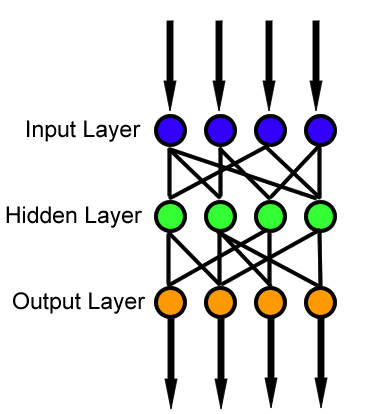
\includegraphics[width=0.7\linewidth]{images/feedforward.png}
        \caption[Feedforward Netz]{Informationsfluss Feedforward Netz \cite{feedforward}}
        \label{fi:feedforward}
    \end{center}
\end{figure}
\subsection{Decision Tree Learning}
\label{sec:dtl}
Entscheidungsbäume (engl. decision tree) werden bei Klassifikationsproblemen eingesetzt, um hierarchisch aufgebaute Entscheidungsregeln darzustellen. Bei jedem Knoten wird ein Attribut abgefragt, und somit der Datensatz immer weiter aufgeteilt, bis ein Blatt erreicht wird. Ein Blatt entspricht dabei der Klassifikation eines durch die vorherigen Knoten definierten Teils des Datensatzes in Bezug auf die Zielklasse. Im Beispiel \ref{fi:entscheidungsbaum} werden Apfelbäume anhand von Apfelbaum-typischen Attributen eingeteilt, um eine Aussage über das Ereignis \glqq Apfelbaum trägt Früchte\grqq{} (Zielklasse) zu treffen.\newline 
Das in \ac{KNIME} genutzte \ac{DTL} Modell basiert auf dem \ac{cart} Algorithmus. Allgemein wählt der \ac{cart} Algorithmus die Attribute zur Trennung der Daten nach der Maximierung des Informationsgehalts der resultierenden Datensätze aus. Hierbei werden Binärbäume generiert. Die Schwellenwerte für die numerischen Attribute an den Knoten, anhand deren die Trennung erfolgt, werden hierbei durch die Optimierung der Entropie der Subsets ermittelt, mit dem Ziel möglichst einheitliche Datensätze in Bezug zur Klasse zu erhalten. Entropie im Sinne der Informationstheorie meint hierbei ein Maß für die \glqq Reinheit\grqq{} bzw. den Informationsgehalt eines Datensatzes (s. Abb. \ref{fi:entropie}). Die Entropie ist dabei wie folgt definiert:
\[Entropie(p) = -\sum_{i=0}^n p_i {\log_2 p_i}\] 
Damit ergibt sich für die linke Menge in der Abbildung \ref{fi:entropie} mit $ p_1=\frac{7}{13}$ und $ p_2=\frac{6}{13}$ eine Entropie von $0,995$, während sich für die rechte Menge mit $ p_1=\frac{13}{13}$ und $ p_2=\frac{0}{13}$ eine Entropie von $0$ ergibt. Simpel ausgedrückt variiert also der Algorithmus die unterschiedlichen Trennungen im Verlauf des Baumes, bis möglichst eindeutige Datensätze in Bezug zur Zielklasse entstehen. Da die Klassifikation hierbei schlussendlich auf Vergleichsoperatoren beruht, ist dieser Algorithmus und auch der generierte Entscheidungsbaum in der Anwendung vergleichsweise schnell. In der Theorie kann der Baum immer weiter wachsen, bis er jeden Einzelfall des Trainingsdatensatzes absolut genau abdeckt. In der Praxis spricht man dabei vom sog. \glqq overfitting\grqq{}. In diesem Fall ist der Baum zu sehr spezialisert, und liefert somit kaum verallgemeinerbare Kenntnisse über die Klassifikation. Deswegen werden der Ausprägung des Entscheidungsbaums in der Praxis, wie auch in \ac{KNIME}, Grenzen gesetzt.
\begin{figure}[H]
    \begin{center}
        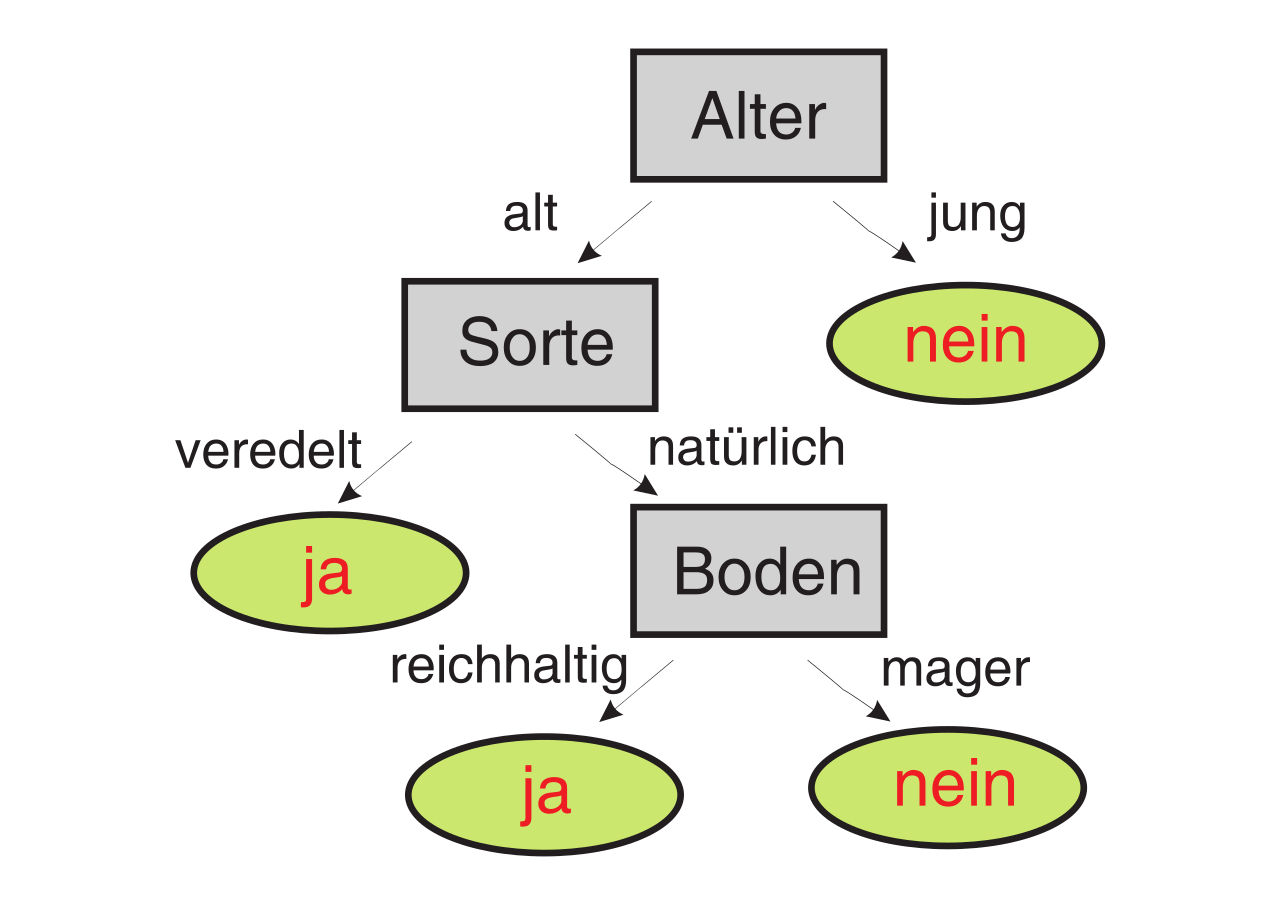
\includegraphics[width=\linewidth]{images/entscheidungsbaum.png}
        \caption[Binärer Entscheidungsbaum]{Binärer Entscheidungsbaum, ob ein Apfelbaum Früchte tragen wird \cite{entscheidungsbaum}}
        \label{fi:entscheidungsbaum}
    \end{center}
\end{figure}
\begin{figure}[H]
    \begin{center}
        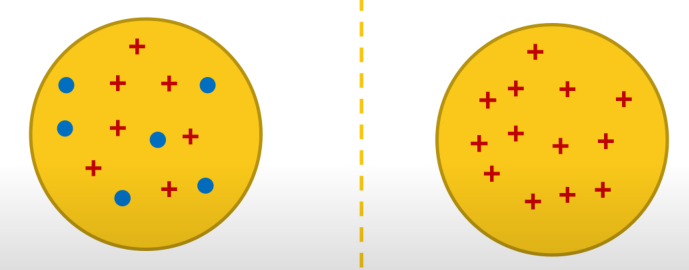
\includegraphics[width=\linewidth]{images/entropie.png}
        \caption[Darstellung Entropie]{Darstellung der Entropie zweier Datensätze mit hoher Entropie (links), und niedriger Entropie (rechts) \cite{entropie}}
        \label{fi:entropie}
    \end{center}
\end{figure}

\chapter{Auswahl untersuchter Filterbauweisen}
\label{ch:auswahl}
Nach Aussage von Karsten Schulz von Freudenberg Filtration Technologies sind Verschleißerscheinungen in Tiefenfiltern nicht relevant. Auslegungs- und Konstruktionsfehler, z.B. beim Design der Strömungskanäle, ausgenommen, sind Tiefenfilter in aller Regel zugesetzt, bevor überhaupt mechanischer Verschleiß auftreten kann.
Im Gegensatz hierzu können Oberflächenfilter, welche mit einem Reinigungsmechanismus ausgestattet sind, durchaus mehrere Jahre in Betrieb sein und abhängig von Wartungsqualität und Belastung bis zu 10 Jahre funktionstüchtig sein. \cite{Schulz} 
Auslegungsfehler können allerdings genauso selbstverständlich auftreten, wie geänderte Rahmenbedingungen (z.B. geänderte Verkehrslage, Baustellen etc.), die eine vorherige Auslegungsrechnung ungültig machen. Es tritt in der Praxis also durchaus auch bei Tiefenfiltern Verschleiß und unvorhergesehene Schäden auf.\newline
Im Kontext dieser Arbeit sind zwei unterschiedliche Vorgehensweise in Bezug auf die beiden Filtertypen Tiefen- und Oberflächenfilter denkbar, welche in den folgenden Unterkapiteln vorgestellt werden.
\section{Filteranlagen mit Abreinigungsmechanismus}
Filteranlagen mit Abreinigungsmechanismus werden häufig bei größeren \ac{lta}'s eingesetzt. Beispiele hierfür wären große Lackierhallen, Produktionshallen, in denen faserverstärkte Werkstoffe bearbeitet werden, oder auch viele spanende Fertigungsverfahren eingesetzt werden. Diese Art von Filteranlagen sind nicht Teil der Arbeit, sollen an dieser Stelle der Vollständigkeit halber jedoch kurz vorgestellt werden, da sie ebenfalls Potenzial für eine KI-basierte Überwachung bieten. \newline
Auf Grund der relativ langen Standzeiten derartiger Filteranlagen ist eine umfangreichere Datenbasis verfügbar bzw. generierbar.
Auf Grund der Fahrweise dieser Anlagen mit abwechselnden Filtrier- und Abreinigungsphasen wäre der zunehmende Verschleiß z.B. an Hand des Vergleichs von erreichten Differenzdruckplateus zwischen Abreinigungsphasen denkbar (s. Abb. \ref{fi:druckverlust_abr}). 
\begin{figure}[H]
    \begin{center}
        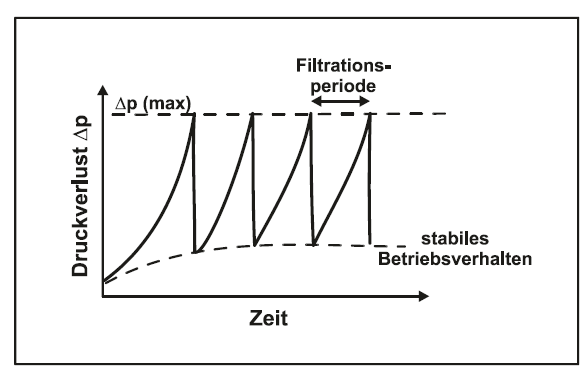
\includegraphics[width=0.55\textwidth]{images/druckverlust_wechsel.png}
        \caption[Druckverlust abreinigende Filter]{Verlauf des Druckverlustes bei Filtern mit Abreinigungsmechanismus \cite{immission} }
        \label{fi:druckverlust_abr}
    \end{center}
\end{figure}
Hieraus ließe sich mit aus Versuchen gewonnenen Daten leicht eine Verschleißkurve generieren, aus der dann Ausfallwahrscheinlichkeiten abgeleitet werden können. Da diese Filteranlagen in der Regel als ein Verbund aus Filterzellen ausgeführt sind, könnte man für die Versuche einzelne Zellen prüfen, was den Realisierungsaufwand reduzieren würde.
Außerdem ständen, im Gegensatz zu Tiefenfiltern, auch Daten aus der Abreinigungsphase zur Verfügung. Diese würden, bei entsprechender Abtastrate, einen guten Indikator für den Verschleißzustand des Filtermediums darstellen, da der Filterkuchen gegen Ende der Abreinigungsphase nahezu vollständig abgetragen wird. Im Filterbetrieb wäre es schwierig Aussagen über den Zustand des Filtermdiums zu treffen, denn der Filterkuchen trägt maßgeblich zur Bildung der Druckdifferenz und Filtrationsleistung bei, und kann somit mechanischen Verschleiß im eigentlichen Filter verschleiern.
\section{Filter zur Raumklimatisierung/lüftung}
In größeren Betriebsgebäuden, wie Bürogebäude, Schulen, Krankenhäuser etc. werden komplexe Lüftungsanlagen zur Klimatisierung und Lüftung eingesetzt. Ziel ist hierbei eine ausreichende Luftqualität und die Vermeidung von Schimmelbildung. Auch die Verbreitung von Keimen und Pilzsporen zu verhindern ist hierbei von Bedeutung, wie die Sars-CoV-2 Pandemie eindrücklich gezeigt hat.
Wie die Keimbelastung von Filtern in Gebäuden überwachbar bzw. vorhersagbar gemacht werden kann ist daher Gegenstand aktueller Forschung. Biologische Vorgänge wie Pilzwachstum oder Virenverbreitung mathematisch beschreibbar zu machen erfordert jedoch einen immensen Versuchsaufwand und die Arbeit eines interdisziplinären Forschungsteams, und soll daher nicht Teil dieser Arbeit sein.\newline
A priori sind vorallem in solchen Szenarien eingesetzte Vorfilter von anhaltender Luftfeuchte und anderen ungünstigen Wetterbedingungen betroffen. Hierbei kann sich die Feuchte in den Filtermedien niederschlagen, was bei einer Überwachung der Differenzdrücke als Überschreitung des Grenzwerts erkannt werden kann. In Konsequenz werden die Filter getauscht, obwohl diese eventuell im laufenden Betrieb getrocknet und im System belassen werden könnten. Die Fusion von Betriebs- und Umweltdaten, wie z.B. Wetterdaten, bietet daher ein vielversprechendes Konzept zur KI-basierten Überwachung solcher Anlagen.
\section{Auswahl anhand beispielhafter Anlage}
\label{sec:auswahl_konk}
Die Auswahl der behandelten Filter erfolgt an einer beispielhaften Klimazentrale (s. Abb. \ref{fi:beispielanlage}), welche aus der VDI3677-2 als typische Anlage übernommen wurde. Die konkrete Auswahl der Filter erfolgt auf Grundlage von Herstellerempfehlungen zur Verwendung der einzelnen Filterklassen. Die Bauweisen werden bei dieser beispielhaften Auswahl bewusst variiert, um anhand des Beispiels die typischen Bauweisen vorzustellen. Für die erste Filterstufe (s. 4 in Abb / Anhang: PSB/290 S) wird ein Grobstaubfilter G4 als Filtermatte verwendet, und dient als Vorfilter zum Schutz der nachgelagerten Systeme der Zuluftseite (unterer Abschnitt Abb. \ref{fi:beispielanlage}). Als zweite Filterstufe (s. 5 in Abb / Anhang: WinAir 90 8M), bzw. Endfilter vor der Verteilung an die Räume, wird ein Feinstaubfilter F7 in Taschenbauweise eingesetzt. Es ist nun üblich für Räume mit besonderen Anforderungen an die Luftqualität sog. endständige Filter in Form von Schwebstofffiltern einzusetzen. Hierfür wird (nicht in Abb. / Anhang: Viledon E11 610x610) im Beispielsystem ein Schwebstofffilter E10 in Kasettenbauweise eingesetzt. Nähere Angaben zu den Filtern in Bezug auf Verschleiß und Analyse der Datenblätter gewählter Filter erfolgt im Kapitel \ref{ch:Filterverschleiß}. Auf die Abluftseite des Systems wird nicht näher eingegangen, da mit dieser Auswahl bereits drei unterschiedliche Filter gemäß Aufgabenstellung \ref{ch: Aufgabenstellung} abgedeckt sind.\newpage
\begin{figure}[H]
    \begin{center}
        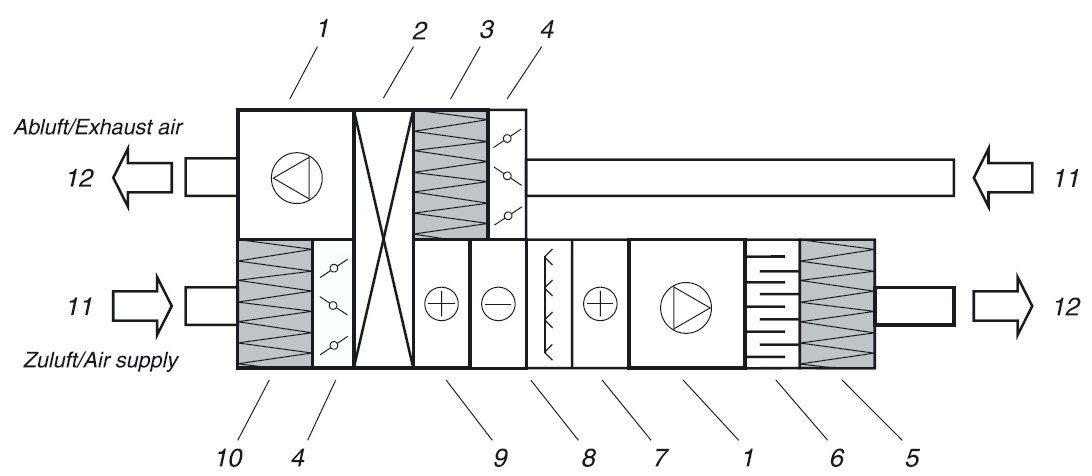
\includegraphics[width=\linewidth]{images/beispielanlage.png}
        \caption[Typische Klimazentrale]{Typischer Aufbau einer  Klimazentrale nach VDI3677-2 \cite{vdi3677_2} }
        \label{fi:beispielanlage}
    \end{center}
\end{figure}
\begin{itemize}
    \item 1 Ventilator
    \item 2 Wärmerückgewinnung
    \item 3 Abluftfilter
    \item 4 Volumenstromregelung
    \item 5 2. Filterstufe
    \item 6 Schalldämpfer
    \item 7 Erhitzer
    \item 8 Befeuchter
    \item 9 Erhitzer/Kühler
    \item 10 1. Filterstufe
    \item 11 Zuluft
    \item 12 Abluft
\end{itemize}






\include{chapters/05Filterverschleiß}

\chapter{Stand der Technik Filterüberwachung}
\label{ch:stand}
    Ziel dieses Kapitels ist einen Überblick über die unterschiedlichen genutzten Technologien zu bieten, die im bearbeiteten Themekomplex den momentanen Stand der Technik darstellen. In Bezug auf Gebäudetechnik ist diese Vorstellung jedoch kritisch zu sehen, da sich die Gebäudetechnik in den letzten Jahrzehnten im Zuge der Digitalisierung, und auch unter Gesichtspunkten wie Energieeffizienz, massiv weiterentwickelt hat. Dies gilt allerdings nur für Neubauten bzw. aufwendige Renovierungsmaßnahmen. Analog hierzu ist in älteren Gebäuden auch entsprechend alte Lüftungs- bzw. Klimatechnik verbaut, welche nicht immer mit modernen Regelungstrategien gesteuert wird, oder gar mit Bus-basierter \ac{glt} ausgestattet ist.
    \section{Direkte Warnsysteme}
    Unter dem Stichwort "Filterbruchüberwachung" lassen sich eine Vielzahl Lösungen finden (s. z.B. \cite{fbu}), um das Versagen unterschiedlicher Filter zu melden. Hierbei wird meist der triboelektrische Effekt genutzt.
    Dieser erzeugt eine zunehmende Messspannung, je mehr Partikel auf den Fühler an der Reingasseite treffen. Wird ein bestimmter Schwellenwert erreicht, wird ein Alarm über die \ac{glt} ausgelöst.
    Diese Art der Überwachung ist als zusätzliche Sicherheitsmaßnahme bei kritischen Anlagenbereichen oder z.B. der Filtration von toxischen Stoffen einzuordnen.
    Eine derartige Überwachung ist im Sinne einer prognostizierenden Überwachung nicht nützlich, da sie systembedingt erst Aufschluss über den Filterzustand geben kann, wenn bereits ein Schaden vorliegt.
    \section{Überwachungsstrategien}
    Üblicherweise wird eine Überwachung der Druckdifferenz am Filter, über eine Differenzmessung mit Schläuchen zur Reingas- und Rohgasseite durchgeführt. Die Messwerte werden dann entweder direkt über die \ac{glt} an eine zentrale Steuerung übertragen, oder zunächst an \ac{ddc}-Stationen auf Feldebene weiterverarbeitet und anschließend Warnungen bzw. Messwerte übertragen. Die Grenzwerte, ob in Feldstation oder Zentrale hinterlegt, basieren hierbei auf einer Mischung aus Herstellerangaben, Erfahrungswerten und Auslegungsrechnungen bei der Installation. 
    \section{Problematik und Grenzen}
    Da momentane Überwachungsstrategien auf der Einhaltung von Grenzwerten basieren, aber hierbei nicht mögliche Umweltfaktoren im Betrieb einbeziehen, lässt sich davon ausgehen, dass grobe Überschlagsrechnungen genutzt werden. Eine detailliertere Auslegung würde den Planungsaufwand nicht rechtfertigen, und auch Versuchsreihen, und hierfür nötige Infrastruktur (z.B. Labore) erforderlich machen. Die resultierenden Kosten stehen nicht im Verhältnis zu den Kosten einer relativ konservativen Auslegung. Dies hat zur Folge, dass die Mehrheit der Filter weit vor Ablauf ihres eigentlichen Lebenszeitendes getauscht werden. Außerdem wird ein Wartungsauftrag zum Tausch in der Regel erst dann ausgelöst, wenn festgelegte Grenzwerte überschritten werden. Selbstverständlich lassen sich hierbei Vorlaufzeiten für Auftragsabwicklung berücksichtigen, im Gegensatz zu prädiktiven Wartungsansätzen ist der Planungs-/Kommunikationsaufwand hierbei jedoch höher. Mit einer prädiktiven Wartung würden sich solche Aufträge hingegen mit ausreichend Vorlaufzeit planen lassen, was auch eventuelle Kosten bei der Abwicklung senkt, da diese z.B. an Schichtpausen, ohne Störung der laufenden Produktion, terminiert werden können.
    \section{Predictive Maintenance}
    \label{sec:predmain}
    Die Instandhaltung von Anlagen ist stets gekoppeltet an den Planungsaufwand, und damit verbundenen Kosten. Weitere Kostenfaktoren können z.B. die Kosten durch die Verschwendung bei der präventiven Instandhaltung sein. Hierbei werden Verschleißteile provisorisch an Hand eines Wartungsplans ausgetauscht.
    Die historische Ausgangslage ist daher die reaktive und präventive Instandhaltung, die auf Erfahrungswerten bzw. Auslegungsberechnungen beruht, wobei bei der reaktiven Instandhaltung nur dann gewartet wird wenn ein Versagen auftritt, und diese somit die einfachste Art der Instandhaltung darstellt. Mit der Einführung der Computer-basierten Überwachung von Maschinendaten erfolgte eine Revolution in der Instandhaltung. Diese Stufe stellt den Ist-Zustand aktueller industrieller Instandhaltungsstrategien dar. Ein sog. \ac{cms} bündelt hierbei Informationen zu Betriebsdaten einzelner Komponenten, analoge Aufgaben in der Gebäudetechnik erfüllt die \ac{glt} mit zentralem Server. Dieses Überwachungssystem wird kontinuierlich mit Messdaten aus permanenten Sensoren versorgt. Somit kann der Zustand der Anlage bzw. Maschine überwacht werden, um aus den gewonnenen Daten Kennwerte zu bilden. Auf Grundlage dieser Kennwerte können dann Instandhaltungsmaßnahmen abgeleitet werden. Dabei ist es möglich die Instandhaltung teilweise zu automatisieren, indem z.B. Grenzwerte für einzelne  Schlüsselparameter festgelegt werden. Hierzu müssen auch Wechselwirkungn einzelner Subsysteme miteinander berücksichtigt werden, was den Aufwand einer Einführung erhöht. Aktueller Stand ist daher die Prognose. Bei dieser Entwicklungsstufe werden statistische Analyseverfahren und Simulationen eingesetzt, um Fehlermuster zu erkennen und Ausfälle vorhersagen zu können. \cite{inst} 
    Der Aufwand steigt hierbei mit der Komplexität der Systeme extrem an, da allgemeingültige Aussagen schwierig zu treffen sind. Gutes Beispiel hierfür ist diese Arbeit, in der kein allgemeingültiges Modell für Luftfilter erstellbar ist, sonder nur für wenige, spezifische Luftfilter. 
    Bei dieser Entwicklungsstufe ist bereits der Einsatz von KI zur Mustererkennung und zur nachgelagerten Prognose auf Basis von Zustandsdaten denkbar.
    Zukünftige Instandhaltungssysteme werden soweit vernetzt sein, dass sie mit Hilfe von Schnittstellen zur Produktionsplanung selbst Instandhaltungsmaßnahmen präventiv auf Grundlage der prognostizierten Auslastung anfordern bzw. planen können. Hierbei wird dann zusätzlich die erwartbare Auslastung einkalkuliert. Eine automatisierte Erstellung von Wartungsaufträgen und ein Versenden dieser an externe Dienstleister ist ebenfalls denkbar. Alleinstellungsmerkmal ist hierbei die dezentrale Interpretation und Analyse von Sensordaten, und zunehmende Befähigung der Systeme auf Feldebene zur Netzwerkkommunikation.  Siehe auch \ref{sec:iiot}. Eine Adaption dieser Entwicklungsstufe auf \ac{lta}'s erscheint weniger sinnvoll, da diese mehr oder weniger kontinuierlich betrieben werden. Die dezentral Verfügbare Rechenleistung bietet jedoch, gerade im Hinblick auf moderne und energieeffiziente Machine Learning Algorithmen, Potenzial zur individuellen Überwachung von Filtern auf Feldebene.
    Denkbar wäre es, an Daten aus Versuchen auf Prüfständen mit einzelnen Filtern angelernte, KI-Modelle in \ac{ddc}-Stationen zu integrieren.


\chapter{Konzepterstellung}
\label{ch:konzept}
    Bei modernen Lüftungsanlagen ist davon auszugehen, dass Betriebsdaten an zentrale Einrichtungen, wie lokale Server zur Überwachung übermittelt werden. Es ist daher sinnvoll an dieser Stelle eine API einzurichten, welche Betriebsdaten an eine Servercloud oder lokale \ac{vm} zum Zweck der Analyse übermittelt. An dieser Datensenke kann dann ein Service zur KI-basierten Analyse bzw. Vorhersage von Schadensfällen eingesetzt werden. Eventuell lassen sich hierfür bereits genutzte Datenbanken einbinden, unter der Vorraussetzung, dass das \ac{ki}-Modell an das Datenmodell angepasst ist, oder alternativ eine Schnittstelle zur Modellierung eingesetzt wird. Die so gewonnenen Zeitverläufe lassen sich dann für die Prognose des Verschleißzustandes nutzen. Das Ziel des Konzeptes ist nicht eine Steuerung, oder Regelung, sondern eine Prognose auf Grundlage historischer und aktueller Zeitverläufe verknüpft mit Verschleißkennwerten. Sie ist somit unabhängig von Echtzeitdaten, und stellt folglich auch keine Echtzeitanforderungen an die Datenübertragung. Vielmehr fußt das Konzept auf Erfahrungswerten aus realen Tests oder robusten bzw. validierten mathematischen Modellen, wobei erstere immer zu einer genaueren Prognose führen werden. 
    Bei einer Anlage die mit Umluft oder Mischluft betrieben wird, werden zusätzliche Modelle erforderlich, die die in den Räumlichkeiten erzeugte Staubbelastung zusätzlich berücksichtigen, welche auf evtl. genormten Belastungen basiert.
    Moderne Anlagen werden als reine Außenluftanlage ausgelegt. Hierbei wird die Außenluft zentral aufbereitet und über ein Kanalnetz an die Räume geleitet. Die verbrauchte Luft wird über ein getrenntes Netz und Abluftventilator aus den Räumen transportiert, wobei im Sinne der Energieeffizienz in der Regel eine Wärmerückgewinnung für das Zuluftsystem erfolgt. \cite{tavg}
    Daher erfolgt die Entwicklung des Konzepts anhand eines reinem Außenluftbetriebes. Im Fort- und Abluftsystem einer solchen Anlage wird dann nur ein Filter zum Schutz des Abluftventilators eingesetzt, esseidenn, es greifen Emissionsschutzvorschriften durch in den Räumen auftrende Schadstoffe.
    Soll die erwartbare Auslastung, im Sinne einer State-of-the-Art Wartungsplanung (s. \ref{sec:predmain}), in die Vorhersage einfließen, werden auch für die Zuluft Informationen bezüglich Staubzusammensetzung und -Last erforderlich. 
\section{Beschreibung gewählter Filterbauart}
    Die in Kap. \ref{sec:auswahl_konk} gewählten Filter sind Tiefenfilter.
    Bei Tiefenfiltern treten allgemein folgende, bereits vorgestellte Filtereffekte auf \cite*{transportvorgänge}:
\begin{itemize}
    \item Sperreffekt
    \item Trägheitseffekt
    \item Diffusionseffekt
\end{itemize}
    Der Einfluss der Effekte schwankt hierbei je nach Volumenstrom, Filterklasse/-Art und Staubzusammensetzung. Entsprechende Kennlinien sind spezifisch für unterschiedliche Filter.Ein vollständiges Konzept müsste diese Einflüsse quantifizieren, um den Rahmen einer Studienarbeit nicht zu überschreiten wird der Volumenstrom im Sinne einer IDA-C4 Regelung gesteuert, die Staubzusammensetzung wird als konstant angenommen (s. \ref{sec:sim} ). 
    Da die Staubzusammensetzung und -konzentration ein bestimmender Faktor für die Beladung der Filter ist, und zeit- und ortsabhängig ist, müsste diese auch in das System einfließen. Dies ist mit Versuchen kaum reproduzierbar, weshalb eine Bewertung des Verschleißzustandes von insbesondere Außenfiltern im realen Betrieb anhand der realen Verläufe eben dieser Größen für die Umsetzung unabdingbar ist.
    Zum Zweck der Darstellung einer Machbarkeit wird nur der E11-Filter (Datenblätter s. Anhang) detaillierter untersucht. Für diesen liegt ausreichend Literatur vor, welche den Einfluss von z.B. Feuchte auf Druckdifferenzverläufe und Verschleiß untersucht. Die nötigen Genauigkeiten für die herausgearbeiteten Messgrößen werden hierbei schon von den meisten low-cost Sensoren erreicht. Eine Evaluation der Abtastraten entfällt, da hier eher minütliche Abtastungen erforderlich sind, was eventuell sogar den Einsatz batteriebetriebener Sensoren ermöglicht. Ausnahme bildet hier die Abtastung der Druckdifferenz im Kontext von möglichen Druckstößen durch Lastwechsel oder Windböen. Die Festlegung der Abtastraten erfordert hierbei Messdaten aus der Praxis, welche dem Verfasser nicht vorliegen.
    \section{Auswahl Sensorik}
    \label{sec:auswahl_sens}
    Ausgehend von Kapitel \ref{sec:ident_mess} müssen die Messgrößen der folgenden Unterkapitel erfasst werden. Im Sinne des Retrofitting bieten sich daher sog. Smarte Sensoren an, um die Möglichkeiten der \ac{lta} zur Messung von Parametern sinnvoll und kosteneffizient zu erweitern. \cite{hybride} Folgend werden jeweils Lösungen zur Messung der unterschiedlichen Parameter vorgestellt. Hierbei ist davon auszugehen, das bereits Einrichtungen zur Messung von Differenzdrücken bzw. Strömung vorhanden sind, aber nicht solche für Temperatur und Feuchte. Für die Größen Temperatur und Feuchte werden daher kompakte, batteriebetriebene Sensoren vorgeschlagen, welche im Verbund mit einem Gateway über Funk, und schließlich über das 4G Mobilfunknetz, Daten in eine Cloud übertragen können. Hierbei wird auch eine REST API bereitgestellt, welche den derzeit quasi-Standard für Event gesteuerte Softwaresysteme darstellt.
    \subsection{Feuchte und Temperatur}
    \label{sec:smartsens}
    Hervorzuheben ist bei diesem Sensor von Disruptive Technologies die extrem kleinen Abmessungen (s. Abb. \ref{fi:feuchtesensor}), sowie die Lebensdauer von etwa 15 Jahren. Durch die Unabhängigkeit von der Stromversorgung würden sich derartige Sensoren ohne großen Aufwand an neuralgischen Punkten der \ac{lta} integrieren lassen. Durch die angesprochene Cloud-Konnektivität würden sie überdies Daten an dem Ort bereitstellen, an dem das vorherig trainierte KI-Modell die Analyse der Daten und Vorhersage der Wartungsfälle übernimmt. Da Feuchte und Temperaturschwankungen naturgemäß eher langsame Vorgänge sind, ist hierbei eine Abtastrate im Minutenbereich ausreichend.
    \begin{figure}[H]
        \begin{center}
            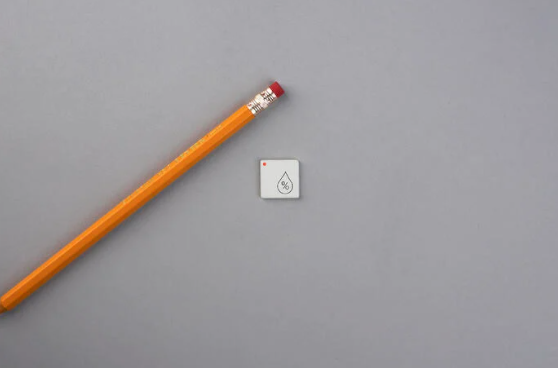
\includegraphics[width=0.8\linewidth]{images/feuchtesensor.png}
            \caption[Feuchtesensor]{Kabelloser Feuchte- und Temperatursensor von Disruptive Technologies \cite{disruptive} }
            \label{fi:feuchtesensor}
        \end{center}
    \end{figure} 
    \subsection{Volumenstrom}
    \label{sec:vstrom}
    Die Erfassung des Volumenstroms erfordert möglicherweise keine zusätzliche Messtechnik, wenn die entsprechenden Werte über die \ac{glt} lesbar sind, bzw. die zuständige Regelungstechnik ausreichend stabil und Netzwerk- oder Busfähig ist. Ist dies nicht gegeben bieten sich zwei verschiedene Lösungen an. Erstens eine Messung über Prandtl Staurohe, mit der Differenz zwischen statischem und dynamischen Druck. Hierbei muss die Messung temperaturkompensiert sein, was analog über eine Messbrücke oder digital über eine integrierte Temperaturmessung an selber Stelle möglich ist. Zweite Möglichkeit ist der Einsatz eines low-cost Strömungssensors, wie in Abbildung \ref{fi:strömsensor} vorgestellt. Durch den Analogausgang mit 0...10 V sollte dieser über Feldstationen in die \ac{glt} integrierbar sein. Ein Messbereich von 0...5\si{\metre\per\second}  sollte hierbei ebenfalls ausreichen. Die Genauigkeit vom vorgeschlagenen low-cost Sensor von $\mp 4\% $ ist hierbei annehmbar, da der Volumenstrom eher als Indikator für die Staubaufnahme zu sehen ist, und daher ohnehin mit einem Koeffizienten über die Zeit kumuliert werden muss.
    \begin{figure}[H]
        \begin{center}
            \includegraphics[width=0.5\linewidth]{images/strömsensor.png}
            \caption[Strömungssensor]{Richtungsunabhängiger low-cost Strömungssensor HLK100 von electro-mation \cite{strömsensor} }
            \label{fi:strömsensor}
        \end{center}
    \end{figure} 
    \subsection{Differenzdruck}
    Zur Messung von Differenzdrücken existieren am Markt eine Vielzahl von Sensoren. Diese Sensoren können ebenso zur Strömungsmessung (s. Kap. \ref{sec:vstrom}) eingesetzt werden.Beispielhaft wurde hier ein Modbus-fähiger Sensor (s. Abb \ref{fi:drucksensor}) ausgewählt. Dieser wäre im Sinne einer modernen \ac{glt} mit Bussystem sinnvoll. Um die Messdaten auch an eine Cloud übermitteln zu können, müsste folglich die zentrale Verarbeitungseinrichtung, wie Anfangs des Kapitels erwähnt, entsprechend ertüchtigt sein. Bei Druckdifferenz ist, im Gegensatz zu den anderen Messgrößen, evtl. eine höhere Abtastrate (Sekunden) nötig, um die in Kap \ref{sec:aufbau} erläuterten Druckschwankungen zu erfassen. Der Messbereich ergibt sich hierbei aus dem jew. Datenblatt, wobei ein Bereich von etwa 0...5 kPa sicherlich alle Fälle abdecken sollte. Dieser Bereich wird von dem vorgestellten Sensor abgedeckt. Die Genauigkeit des Sensors von $\mp 3\% EW$ reicht für den Zweck der Überwachung ebenfalls aus, da der Differenzdruck vermutlich als einer von vielen Grenzwerten realisiert wird. 
    \begin{figure}[H]
        \begin{center}
            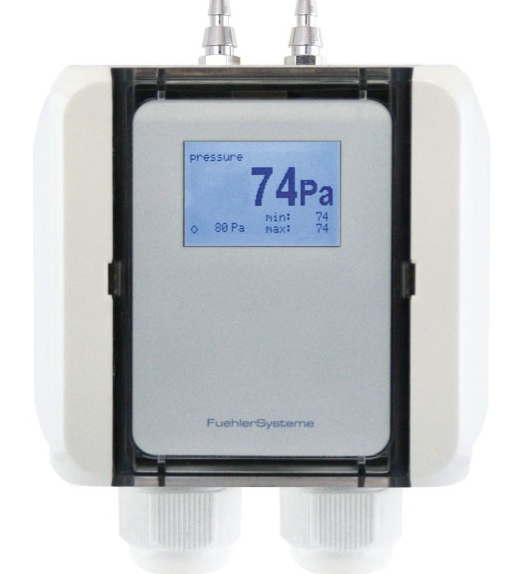
\includegraphics[width=0.5\linewidth]{images/drucksensor.png}
            \caption[Differenzdruck Messumformer]{Modbus-fähiger Drucksensor für Differenzdruck FS1200 von FühlerSysteme eNET \cite{drucksensor} }
            \label{fi:drucksensor}
        \end{center}
    \end{figure} 
    \section{Auswahl Systemarchitektur}
    Auf Basis (s. Kapitel \ref{sec:aufbau}) wird ein belegungsgesteuerter Volumenstrom mit zentraler Anlage angesetzt. Dies macht eine Erfassung von Volumenstromdaten erforderlich, um die Staubbeladung modellieren zu können. Die Frage an welchem Punkt im System dies geschieht, muss vom Aufbau der Anlage abhängig gemacht werden, es bietet sich jedoch an möglichst nah vor der Filtern derartige Messpunkte zu integrieren. Hierbei müssen eventuelle Leitungswiderstände aus der Oberfläche und Geometrie (Knicke etc.) der Schächte berücksichtigt werden. Bei Nutzung von KI ist dies jedoch nicht erforderlich, da diese Zusammenhänge von der KI "erlernt" werden können. Die Eingangsgrößen für das Modell wurden bereits in Kapitel \ref{sec:ident_mess} bzw. \ref{sec:umweltbed} erläutert. Die Messung von Klimadaten innerhalb der \ac{lta} sollte, unter der Annahme gleichbleibender bzw. vergleichbarer Werte innerhalb des Systems, kurz hinter dem Zuluftsystem ausreichen. Somit ist an den Filtern nur die Messung der Druckdifferenz einzusetzen, welche an Kanäle entsprechender Daten vom Zuluftsystem angebunden ist. Alternativ sind die Daten aus Zuluftsystem und Umgebung in einer lokalen Datenbank/Cloud verfügbar, und enstprechende \ac{api}'s z.B. zur Abfrage von Umweltdaten von Servern des Umweltbundesamtes eingerichtet (siehe \cite{webhookUBA}). Die Abbildung \ref{fi:architektur} zeigt hierbei die beispielhafte Umsetzung eines solchen Konzepts. Die relevanten Daten werden über unterschiedliche Protokolle an einen Cloud Server gesendet und dort analysiert. Es bietet sich in diesem Kontext an eine lokale Wetterstation in der Nähe der Zuluftseite außerhalb des Gebäudes zu installieren. Eine Wetterstation zu diesem Zweck ist in der Regel nicht kosteninstensiv, einfach zu installieren, und oftmals bereits für \ac{iot} Protokolle ausgerüstet und vorkonfiguriert. Die Messung von Differenzdrücken und Strömungsgeschwindigkeit wird über eine busfähige \ac{glt} an einen lokalen Server übermittelt, welcher die Daten über ein Webprotokoll an die Cloud weitergibt. Die Erfassung von Klimadaten innerhalb der Anlage erfolgt über die in Kapitel \ref{sec:smartsens} vorgestellten Smart Sensors. Da für die Abtastrate der Daten relativ geringe Anforderungen bestehen, ist die Wahl der Protkolle und \ac{api}'s hinsichtlich Bandbreite und Echtzeitfähigkeit unkritisch, und sollte anhand von Integrationsaufwand und Anschaffungskosten erfolgen.
    \begin{figure}[H]
        \begin{center}
            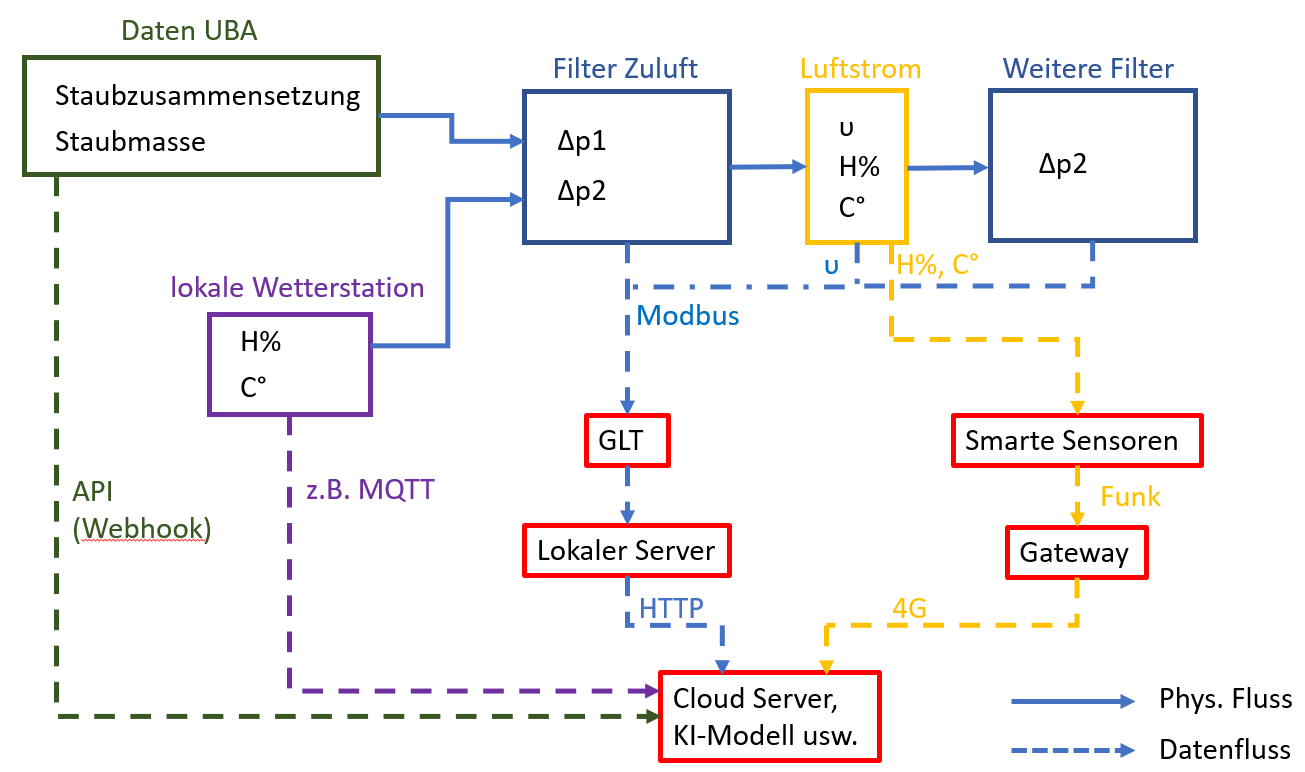
\includegraphics[width=\linewidth]{images/architektur.png}
            \caption[Architektur des Konzepts]{Beispielhafte Architektur des Konzepts}
            \label{fi:architektur}
        \end{center}
    \end{figure} 
    \section{Erforderliche Versuchsreihen}
    \label{sec:versuchsreihen}
    Angelehnt an die Untersuchungen von Bergmann \cite{hepa} und Ricketts \cite{feuchte} wäre es sinnvoll die bis zur Zerstörung erreichten Differenzdrücke an unterschiedlichen Proben der Filter zu untersuchen. Hierzu müssen konstante Prüfbedingungen, bestenfalls in Anlehnung an die Normen DIN EN ISO 16890 \cite{16890}, sowie DIN EN 1822 \cite{1822}, hergestellt werden.
    Optimal wäre es hierbei, Filterproben unterschiedlicher Einsatzdauer und hiermit verknüpfte, historische Daten zu den in Kap. \ref{sec:ident_mess} genannten Messgrößen, zerstörend zu prüfen, eventuell auch Zugversuche oder Berstdrucktests durchzuführen. Alternativ bzw. zusätzlich wären möglichst viele Versuchsreihen mit variablen Parametern sinnvoll, wenn dabei betriebsähnliche Bedingungen simuliert werden können. Hierbei wäre ein konstant halten der einzelnen Parameter nicht entscheidend für den Erfolg, sondern vielmehr die genaue messtechnische Erfassung und ausreichende Anzahl an Durchläufen, um eine zusätzliche Datenbasis für das KI-Modell zu generieren. Dies stellt auch den Vorteil einer KI-basierten Überwachung heraus, da hierfür nicht derselbe Aufwand betrieben werden muss, wie er nötig wäre um einzelne Zusammenhänge, z.B. den Einfluss von Luftfeuchte auf erreichte Enddruckdifferenzen, zu prüfen. Denn bei der Ermittlung derartiger mathematisch-physikalischen Zusammenhänge müssten bestimmte Einflussgrößen konstant gehalten werden, während andere variiert werden, was eine Entwicklung entsprechender Regelungen und Aktorik voraussetzt.
    \section{Funktionsweise}
    \label{sec:funktionsweise}
    Ziel des KI-Modells ist also die Vorhersage des Versagens eines Filters, bevor dieser auftritt, in einem bestimmten Vorhersagehorizont. Dieser Vorhersagehorizont ist abhängig von der Reaktionszeit bzw. den Gegebenheiten vor Ort, und kann auch von Kosten abhängig sein. Beispielsweise deckt ein Vorhersagehorizont von einer Woche mit Sicherheit Werktage ab, während bei einem kleineren Vorhersagehorizont evtl. zusätzliche Kosten durch z.B. Wochenendzuschläge entstehen können.
    Eingangsgrößen für die Vorhersage sind: Feuchte, Temperatur, Staubzusammensetzung, Volumenstrom und Druckdifferenz, wie in Kap. \ref{sec:auswahl_sens} und Kap. \ref{sec:ident_mess} vorgestellt. Die Standzeit kann durchaus ebenfalls relevant sein, wenn Alterungseffekte für das Filtermedium relevant sind. \\
    Allgemein wird der Vorhersagehorizont erreicht, in dem ein KI-Modell mit Fehlerdaten angelernt wird, die mit vergangenen Eingangsgrößen verknüft sind. In der Anwendung resultiert hieraus, dass die KI mit IST-Werten, innerhalb einer gewissen Unschärfe, die Zukunft vorhersagen kann. Hierbei müssen die Daten vorher aufbereitet werden, was z.B. Kumulation oder Mittelwertsbildung vergangener Werte eines Filters einschließt (s. Kap. \ref{sec:knime}). Die Festlegung dieser Aufbereitungsverfahren erfordert Domänenwissen, was durch die Analyse von bisherigen Verläufen und Kenntnisse über Luftfilter einschließt. Die Bereitstellung der Daten erfolgt auf Feldebene bestenfalls durch den Einsaz von Smart-Sensors (s. Kap. \ref{sec:auswahl_sens}), und die Verknüpfung darüber hinaus mit einer busfähigen \ac{glt}. Die Software \ac{KNIME} bietet hierfür bereits sowohl die Möglichkeit z.B. eine SQL-Datenbank abzufragen, in welcher die Messdaten gespeichert sein könnten, als auch die Möglichkeit Alarme über gängige Web-API's zu implementieren. Die konkrete Integration eines solchen Konzepts soll in dieser Arbeit nicht vorgestellt werden, da diese von zu vielen Umständen, wie vorhandene Serverinfrastruktur, Art der bisherigen Wartungsplanung(-software) usw., abhängig ist.

\chapter{Validierung des entwickelten Konzepts}
\label{ch:validierung}
Eine Validierung im Sinne der Verifizierung von Ergebnissen aus der Praxis entfällt im Rahmen dieser Arbeit. Es wird jedoch ein Simulationsmodell anhand von, in folgenden Kapiteln beschriebener, Vereinfachungen und Annäherungen aus realen Versuchsreihen an vergleichbaren Filtern aufgebaut. Das Simulationsmodell generiert hierbei Verläufe der in Kap. \ref{sec:ident_mess} ermittelten Messgrößen, mit Ausnahme der Temperatur, bis zum simulierten Versagen des Filters in Folge mechanischer Überbeanspruchung. Die so generierten Verläufe werden dann im zweiten Abschnitt der Validierung mit \ac{KNIME} untersucht, und ein \ac{ki}-Modell trainiert. Das Modell wird dann mit einem separaten Testdatensatz gespeist, um die Vorhersagegenauigkeit des Modells zu evaluieren. Das Potenzial eines derartigen prädiktiven Warnsystems werden in der Schlussbetrachtung \ref{ch:schluss} gesondert vorgestellt.
Da der Volumenstrom als Rechtecksignal simuliert wird, ist nicht von einer Verschiebung der Filtereffekte auszugehen, was sich auf die Fraktionsabscheidegrade auswirken würde, da sich somit der Filter im lt. Datenblatt empfohlenen Betriebsbereich befindet (s. Kap. \ref{sec:regelungsart}). Auf eine Simulation der Filtereffekte bie unterschiedlichen Strömugsgeschwindigkeiten wird daher verzichtet.
    \section{Erstellung Matlab/Simulink Modell}
    \label{sec:sim}
    Da im Rahmen der Arbeit keine Versuche mit Filtern vorgesehen sind, müssen für eine nachgelagerte KI-basierte Analyse die Trainingsdaten mit Hilfe einer Simulation generiert werden. Hierzu wird ein Modell in MatLab/Simulink erstellt, welches das Verhalten des Filters in Abhängigkeit von Umgebungsparametern und Volumenstrom abbildet. Da die Arbeit ein Proof-of-Concept darstellt, und nicht den Anspruch einer integrationsreifen Lösung hat, werden Annahmen für diverse Verläufe und Zusammenhänge getroffen. Der Einfluss der Temperaturen wird nicht berücksichtigt, da die Modellierung von z.B. Taupunkten und der Einfluss auf mech. Eigenschaften eine zu hohe Komplexität in Relation zum Zweck der Simulation erfordert. Die Simulation gliedert sich in das m-file, welche die Eingangsparameter und -berechnungen liefert (s. Abb. \ref{fi:mfile_parameter}), sowie die Simulation selbst (s. Abb. \ref{fi:sim_aufbau}). Da möglichst viele Reihen simuliert werden müssen, entspricht, um die Durchlaufzeit zu verringern, die Simulationszeiteinheit einer Stunde in der Realität.
    \begin{figure}[H]
        \begin{center}
            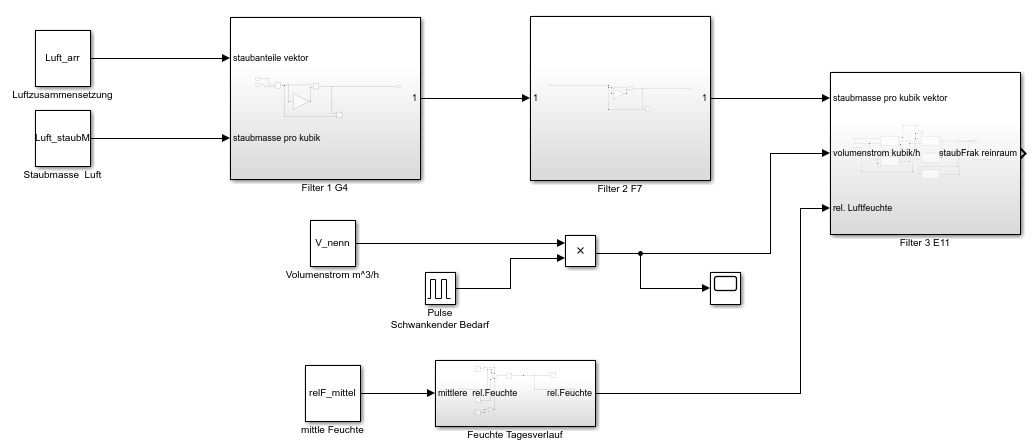
\includegraphics[width=\linewidth]{images/sim_aufbau.png}
            \caption[Aufbau Simulation]{Aufbau der Simulation}
            \label{fi:sim_aufbau}
        \end{center}
    \end{figure}
    Die Simulation ist dabei modular, dem Aufbau des Beispielsystems (s. Kap. \ref{sec:auswahl_konk}) folgend, in einzelne Filter unterteilt. Da der endständige Filter genauer untersucht werden soll, wurden die vorherigen Filter nur als Einfluss auf die Staubanteile und -masse modelliert (s. Abb. \ref{fi:sim_vorfilter}). Hierbei sind die Eingangsgrößen für beide Vorfilter die Staubmasse als Variable, sowie die Staubanteile als eindimensionaler Vektor. Durch Multiplikation miteinandern wird der Vektor zur Darstellung der Staubmasse in \si{\gram} pro \si{\cubic\meter}. Anschließend wird von den einzelnen Werten der Anteil subtrahiert, den der jeweilige Vorfilter zurückhält. Die Fraktionsabscheidegrade der Filter wurden vorher in eine Excel Datei eingetragen, welche vom m-file Skript eingelesen, und als Array behandelt werden. Hierbei ist anzumerken, das die Fraktionsabscheidegrade nicht direkt in den Datenblättern angegeben sind, sondern diese empirisch anhand von rechnerischen Abschätzungen zum Gesamtabscheidegrad bzw. Normangaben bestimmt wurden. Ausgangsgröße der Vorfiltermodule ist also ein Vektor, der die Staubmasse pro Volumen der einzelnen Staubfraktionen darstellt.
    \begin{figure}[H]
        \begin{center}
            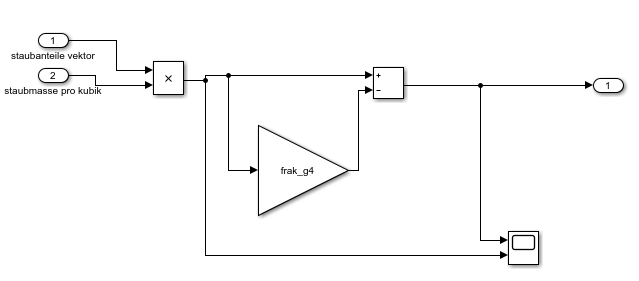
\includegraphics[width=\linewidth]{images/sim_vorfilter.png}
            \caption[Simulation der Vorfilter]{Simulation der Vorfilter}
            \label{fi:sim_vorfilter}
        \end{center}
    \end{figure}
    \subsection{Eingangsparameter}
    Die Staubzusammensetzung der Außenluft wurde nach Abb \ref{fi:staubanteile}, sowie Informationen des Umweltbundesamtes zur Staublast \cite{uba_pm10} als Array implementiert (s. Abb. \ref{fi:mfile_parameter}). Hierbei wurden jeweils Jahresmittelwerte genutzt; eine Simulation der jahreszeitlichen Schwankungen entfällt.
    \begin{figure}[H]
        \begin{center}
            \includegraphics[width=\linewidth]{images/außenluft.png}
            \caption[Außenluft Zusammensetzung]{Mittlere Staubanteile in Großstadtluft \cite{Grundlagen_Filtertechnik}}
            \label{fi:staubanteile}
        \end{center}
    \end{figure}
Da bei Fein- und Schwebstoffiltern keine Angabe zum Staubspeichervermögen gemacht werden, werden im Fall des genutzten E11-Filters Annahmen auf Grundlagen der Untersuchungen von Bergmann zu HEPA Filtern \cite{hepa} getroffen. Da sich die Umsetzung des Konzepts auf den E11-Filter konzentriert, werden analoge Berechnungen für den F7-Filter nicht durchgeführt.
Grundlage bilden dabei folgende Filterparameter \ref{fi:filterparameter}, sowie die von Bergmann ermittelten Druckdifferenzverläufe bei trockener Luft und Beaufschlagung mit Aluminiumhydroxid. Die Tabelle \ref{tab:beladungE11} zeigt hierbei die Ergebnisse der Berechnungen zur Beladung in Gramm pro \si{\square\meter} bei den untersuchten \ac{hepa} Filtern. Da die Berechnung der effektiven Fläche auch geometrische Angaben der Falten erfordern, diese aber nicht in Produktdatenblättern (s. Anhang) vermerkt sind, wird ein Faktor zur Umrechnung der Einbaufläche in effektive Fläche aufgestellt. Im Falle der von Bergmann untersuchten Filter ist die Einbaufläche \[ 18,5 in. * 23 in. = 1,285 sq. ft. \] bei einer effektiven Filterfläche von \[ 308 sq. ft. \]. Damit ergibt sich ein Faktor von \[
    240 = \frac{308 sq. ft.}{1,285 sq. ft.}
    \] für dieses Verhältnis. Da diese Filter eine Tiefe von 3 in. haben, wird der Faktor auf die Viledon Filter mit einer Faltentiefe von 100 mm angewendet. Selbstverständlich ist dieser Vergleich nicht unbedingt zulässig. Schon kleine Änderungen in der Faltengeometrie haben relativ große Auswirkungen auf die effektive Fläche, das Ziel der Arbeit ist jedoch die Vorstellung des Überwachungskonzepts, und nicht die genaue Umsetzung einer Simulation von Filtern.
    Für die Einbaugröße 610 mm x 610 mm = 0,3721 \si{\square\meter} ergibt sich hieraus mit dem Faktor 240 eine effektive Fläche von 89,3 \si{\square\meter}. Die mittlere Beladung pro \si{\square\meter} ergibt sich nach den Ergebnissen aus Tabelle \ref{tab:beladungE11} zu 14,165 \si{ \gram\per\square\metre}. Weitere geometrische Parameter wurden in Anlehnung an Bergman in metrische Einheiten umgerechnet, insofern diese nicht im Datenblatt vermerkt sind. Die entsprechenden so ermittelten Eingangsparameter wurden über das m-file implementiert (s. Abb. \ref{fi:mfile_parameter}).
\begin{figure}[H]
    \begin{center}
        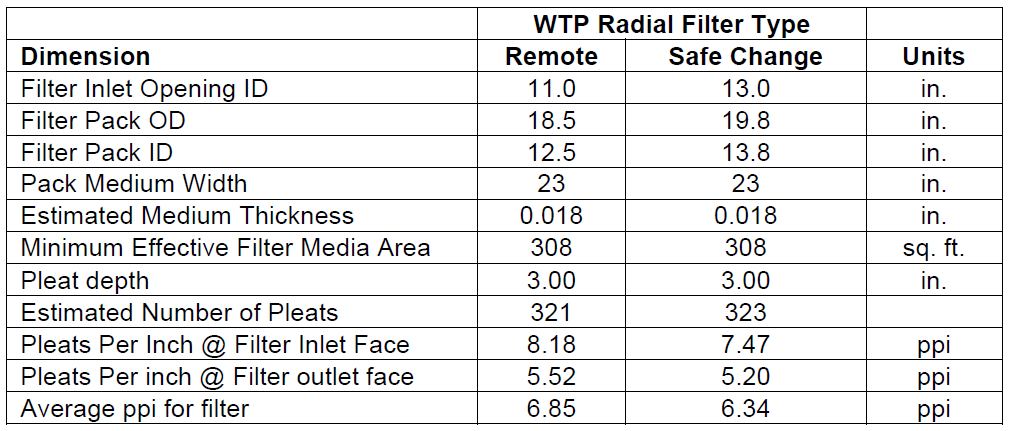
\includegraphics[width=\linewidth]{images/filter_dimensionen.png}
        \caption[Parameter HEPA Filter Bergmann]{Filterparameter untersuchter \ac{hepa} Filter von Bergmann \cite{hepa}}
        \label{fi:filterparameter}
    \end{center}
\end{figure}
\begin{table}[]
    \caption{Beladung und Druckdifferenz der Filter}
    \begin{tabular}{lllllll}
    Filter Nr. & in. WC & Druck {[}Pa{]} & Masse {[}g{]} & Fläche {[}sq.ft.{]} & Fläche{[}m2{]} & Beladung{[}g/m2{]} \\
    1          & 4      & 995            & 440           & 308                 & 28,6141        & 15,4               \\
    2          & 4      & 995            & 370           & 308                 & 28,6141        & 12,93             
    \end{tabular}
    \label{tab:beladungE11}
    \end{table}
Der Jahresmittelwert der  Staubbelastung (PM10) in Wolfsburg beträgt nach Messungen des Umweltbundesamtes 12 \si{\micro\gram\per\cubic\metre}. Wird der Massenanteil für Grobstaub nach \ref{fi:staubanteile} mit einbezogen, ergibt dies einen gesamten Massenanteil von 15,36 \si{\micro\gram\per\cubic\metre}.
    \begin{figure}[H]
        \begin{center}
            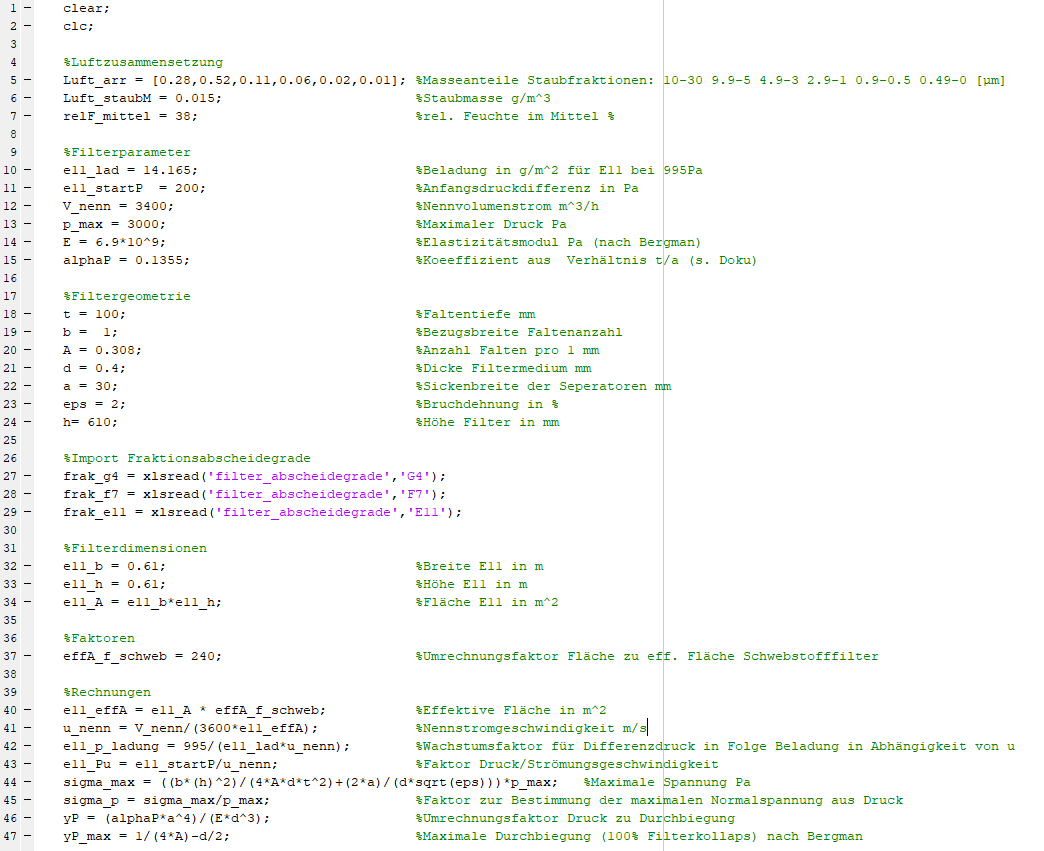
\includegraphics[width=\linewidth]{images/mfile_parameter.png}
            \caption[M-file Simulink]{Eingangsparameter und -rechnungen in m-File}
            \label{fi:mfile_parameter}
        \end{center}
    \end{figure}
    Kern der Simulation ist das Verhalten des E11 Filters (s. Abb. \ref{fi:sim_e11}). Eingangsgrößen sind hierbei der bereits erläuterte Vektor der Staubanteile, der Volumenstrom in \si{\cubic\metre\per\hour}, und die relative Luftfeuchte in \%. Essenziell für die Simulation des Filters sind zwei Subsysteme. Das Subsystem Filterleistung (s. Abb. \ref{fi:sim_filterleistung}) liefert als erste Ausgangsgröße, analog zu den Vorfiltern, die Staubanteile an der Reingasseite. Desweiteren wird die gesamte Staubmasse aus dem Eingangsvektor der Staubanteile summiert, über die Simulationszeit integriert, und mit der effektiven Filterfläche aus dem m-file zur gesamten Beladung des Filters in \si{\gram\per\square\metre} berechnet. Das zweite grundlegende Subsystem berechnet die Strömungsgeschwindigkeit aus dem Volumenstrom und der effektiven Filterfläche in \si{\metre\per\second}.
    Die weiteren Subsysteme, welche Berechnungen der mechanischen Last, Druckdifferenz usw. beinhalten, werden in den folgenden Kapiteln vorgestellt.
    \begin{figure}[H]
        \begin{center}
            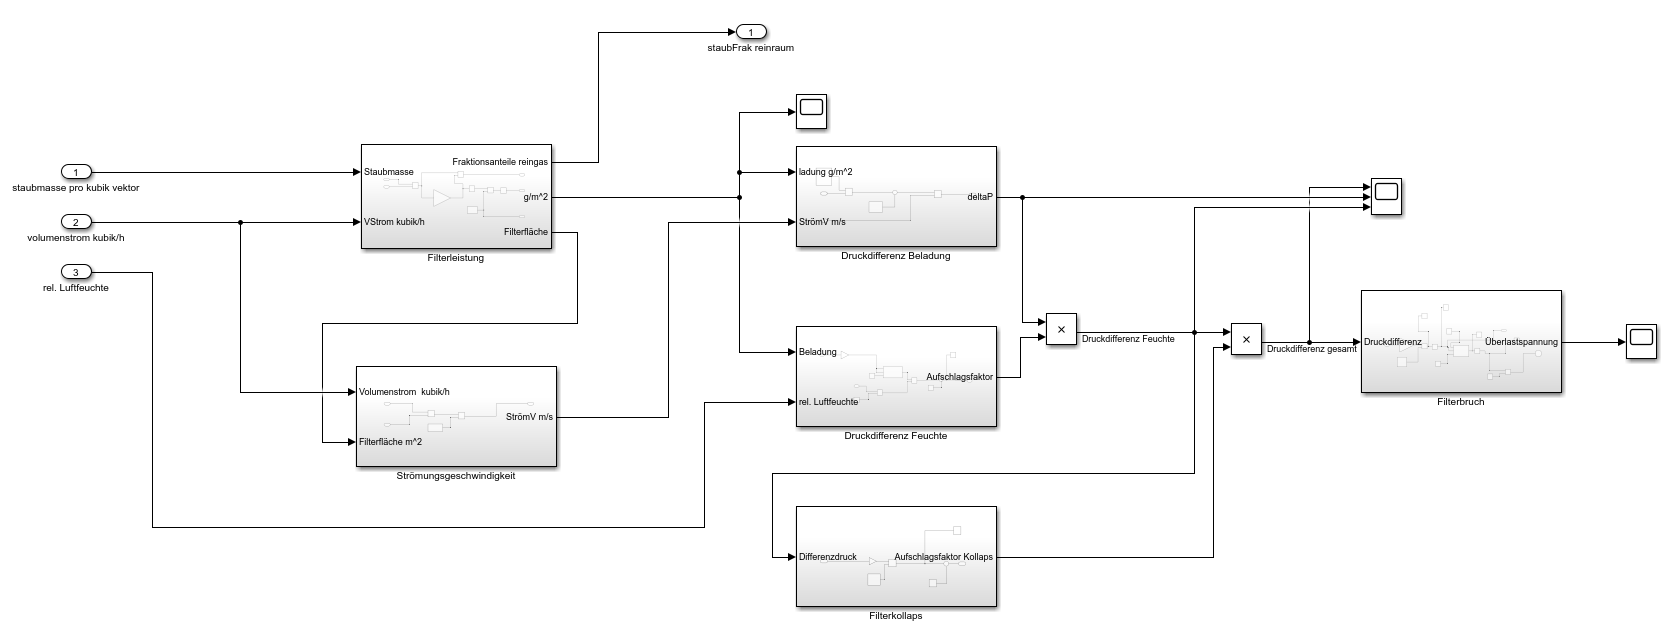
\includegraphics[width=\linewidth]{images/sim_e11.png}
            \caption[Simulation E11 Filter]{Subsystem der Simulation: endständiger E11 Filter}
            \label{fi:sim_e11}
        \end{center}
    \end{figure}
    \begin{figure}[H]
        \begin{center}
            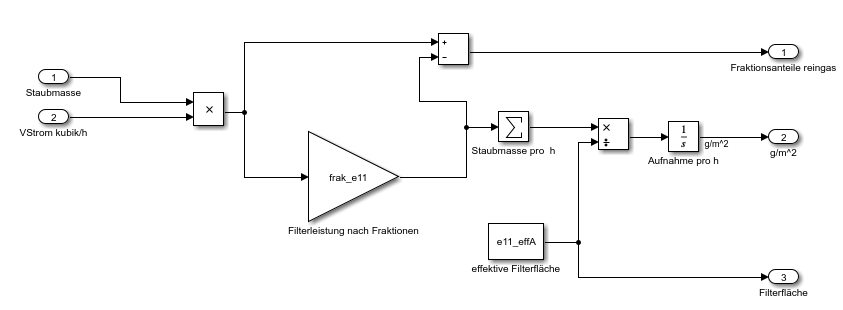
\includegraphics[width=\linewidth]{images/sim_filterleistung.png}
            \caption[Subsystem Filterleistung]{Subsystem der Simulation: Filterleistung des E11 Filters}
            \label{fi:sim_filterleistung}
        \end{center}
    \end{figure}
    \subsection{Druckverlust Beladung}
    "Der Druckverlust von Faserfiltern steigt infolge der Partikeleinlagerung im Filtermedium
mit der Zeit an. Dieses Phänomen ist bekannt, jedoch ist bis zum heutigen Wissensstand
keine gesicherte Vorausberechnung des Druckverlustanstiegs infolge der Partikelbeladung
in Faserfiltern möglich. Man ist demzufolge auf Experimente angewiesen."\cite{reinraum}
Um diesen Zusammenhang dennoch modellhaft darstellen zu können, wird vom unbeladenen Zustand bis zur empfohlenen Enddruckdifferenz bzw. Erreichen der Speicherkapazität, ein linearer Verlauf der Druckdifferenz angenommen. Die entsprechende Berechnung erfolgt im Subsystem "Druckdifferenz Beladung" (s. Abb. \ref{fi:sim_beladung}) als lineares Wachstum, wofür im m-file (s. Abb. \ref{fi:mfile_parameter}) ein Faktor für die Steigung aus Angaben des Datenblatts berechnet wird. Ausgangsgröße ist die Druckdifferenz in Pascal.
\begin{figure}[H]
    \begin{center}
        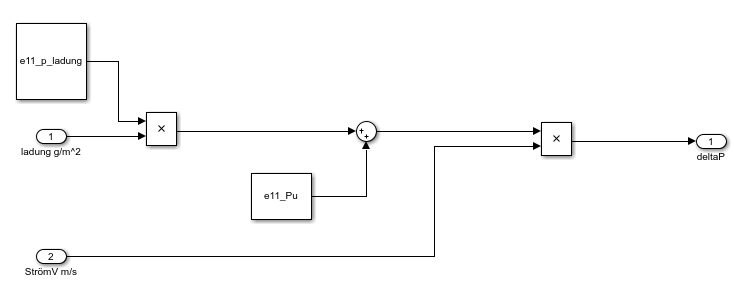
\includegraphics[width=\linewidth]{images/sim_beladung.png}
        \caption[Subsystem Druckdifferenz Beladung]{Subsystem der Simulation: Druckdifferenz durch Beladung des E11 Filters}
        \label{fi:sim_beladung}
    \end{center}
\end{figure}
\subsection{Feuchte}
Für die Modellierung des Druckverlusts in Folge hoher rel. Luftfeuchten wird die Dissertation von Ricketts' zu diesem Thema mit Bezug auf Schwebstofffiltern \cite{feuchte} zurückgegriffen. Ricketts stellt hierbei eine Grundlage zur Berechnung der steigenden Druckdifferenz in Folge von hoher Feuchte über eine bestimmte Einwirkzeit auf. Abbildung \ref{fi:parameter} verdeutlicht außerdem die Vielzahl an Einflussparametern auf den Druckwiderstand von Schwebstofffiltern, was bedingt auch auf andere Filterklassen übertragbar ist. Die Vielzahl der Parameter (s. Abb. \ref{fi:parameter}) zeigt, dass realitätsnahe Daten nahezu unmöglich mit einer Simulation generierbar sind. Die untersuchten Filter sind mit Hinblick auf die Werkstoffe der Filtermedien mit heutigen \ac{hepa} Filtern vergleichbar, da Glasfaserfiltermedien verwendet wurden. \newline
Die Sorption von Wasser durch Filter ist stark von der Staubbeladung und der Art des Staubes abhängig, da dieser Kapazitäten zur Wasseraufnahme bereitstellt. Beispielsweise wird ein Staub mit überwiegend hydrophoben Eigenschaften evtl. sogar die Aufnahme von Wasser bei gleicher Feuchte und Strömungsgeschwindigkeit verringern. \cite{feuchte} 
Die rel. Feuchte der Luft bestimmt das Gleichgewicht zwischen Adsorptions- bzw. Absorptions- und Desorptionsrate. Dies ist durch sog. Sorptionsisotherme charakterisiert, welche in der Regel empirisch ermittelt werden. In der regel stabilisiert sich die eingelagerte Wassermenge bei konstanten Parametern und ausreichend langer Einwirkzeit. Ricketts ermittelt über 70\% rel. Feuchte eine verstärkte Wassereinlagerung im Filter, und in Folge eine Änderung der Druckdifferenz (s. Abb. \ref{fi:feuchte_1}).
\begin{figure}[H]
    \begin{center}
        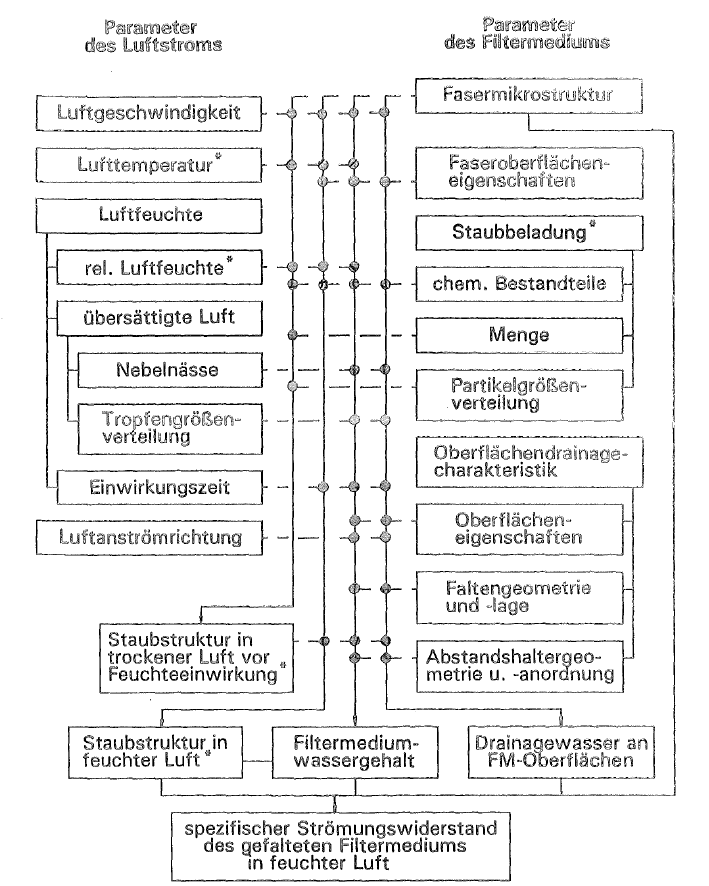
\includegraphics[width=1.1\linewidth]{images/parameter.png}
        \caption[Einflussparameter Ricketts]{Luftstrom- und Filtermediumparameter mit Einfluss auf den Strömungswiderstand von Schwebstofffiltern nach Ricketts \cite{feuchte}}
        \label{fi:parameter}
    \end{center}
\end{figure}
\begin{figure}[H]
    \begin{center}
        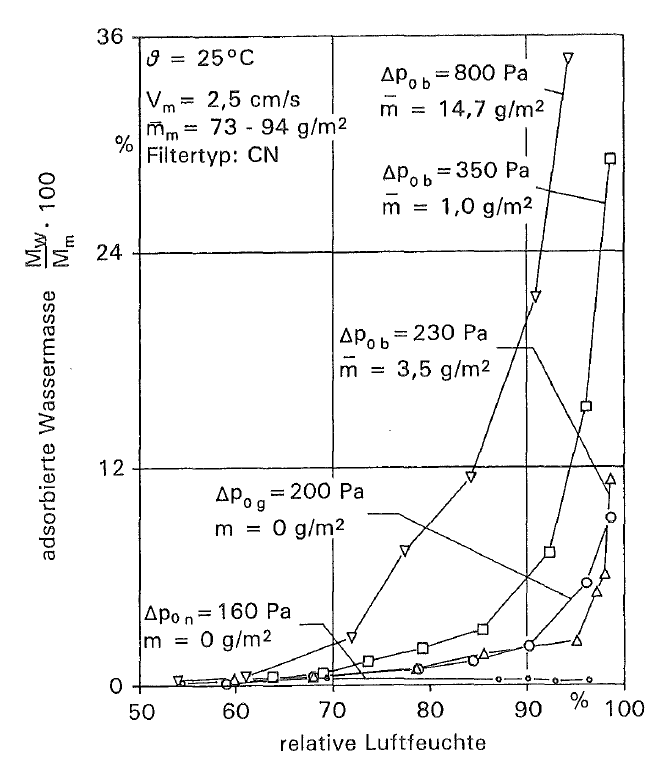
\includegraphics[width=0.95\linewidth]{images/feuchte_1.png}
        \caption[Materialfeuchte rel. Luftfeuchte]{Absorptionstherme von Filterproben in verschiedenen Zuständen \cite{feuchte} S.55}
        \label{fi:feuchte_1}
    \end{center}
\end{figure}
   Der Einfluss der Materialfeuchte auf die Druckdifferenz ist ein zeitabhängiger Vorgang und der Verlauf der Druckdifferenz ähnelt hierbei einer Sättigungskurve auf den etwa dreifachen Wert (s. Abb. \ref{fi:feuchte_2}). Eine Modellierung der Zeitabhängigkeit der Feuchteaufnahme und Druckdifferenz in der Simulation wäre wünschenswert, trägt aber nicht zum Ziel der Arbeit bei. Die Verläufe müssen in jedem Fall empirisch an Filterproben mit unterschiedlichem Beladungszustand und Feuchte ermittelt werden, um eine genaue Modellerierung zu gewährleisten. Wurden diese Verläufe erfasst, bestenfalls unter Verwendung von \ac{doe} Methoden, liegt bereits eine extensive Datenbasis vor, für die sich eine KI basierte Analyse anbietet. 
   \begin{figure}[H]
    \begin{center}
        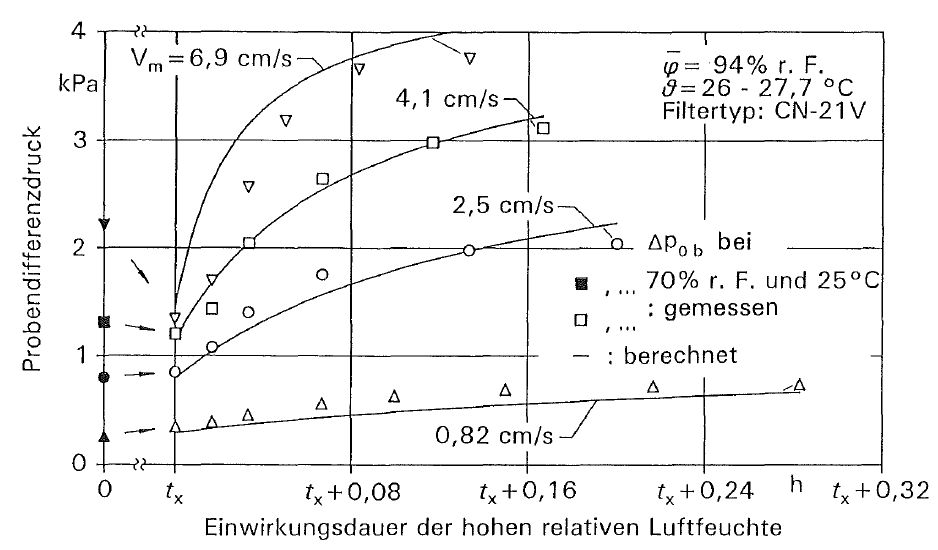
\includegraphics[width=0.9\linewidth]{images/feuchte_2.png}
        \caption[Differenzdruckverläufe Filterproben]{Differenzdruckverläufe der Proben bei unterschiedlichen Anströmgeschwindigkeiten \cite{feuchte} S.72}
        \label{fi:feuchte_2}
    \end{center}
\end{figure}
    Im Modul "Druckdifferenz Feuchte" wird (s. Abb. \ref{fi:sim_feuchte}) zunächst der Feuchtewert von Prozent in einen Dezimalwert umgerechnet. Der Switch-Block gibt den Feuchtewert nur überhalb 70\% weiter. Die Einwirkzeit wird bei erstellten Modul nicht berücksichtigt. Jedoch wird der Wert der Feuchte mit der Beladung verrechnet und ein Aufschlagsfaktor gebildet, so dass bei 100\% rel. Feuchte und 15 \si{\gram\per\square\metre} (nachträglich in Sim. korrigiert) eine Verdopplung der Druckdifferenz eintritt. Dieser Faktor wurde auf Grundlage der erreichten Druckdifferenzen von 800 bzw. 350 Pascal der mit 14,7 bzw. 1 \si{\gram\per\square\metre} beladenen Proben aus Abb. \ref{fi:feuchte_1} approximiert.
    \begin{figure}[H]
        \begin{center}
            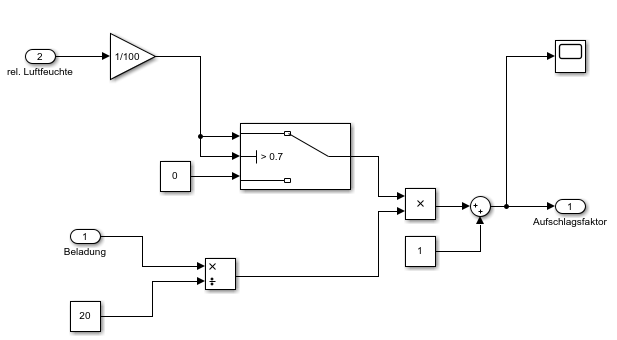
\includegraphics[width=0.9\linewidth]{images/sim_feuchte.png}
            \caption[Subsystem Druckdifferenz Feuchte]{Subsystem der Simulation: Druckdifferenz durch Feuchteeinwirkung auf den E11 Filter}
            \label{fi:sim_feuchte}
        \end{center}
    \end{figure}
\begin{figure}
    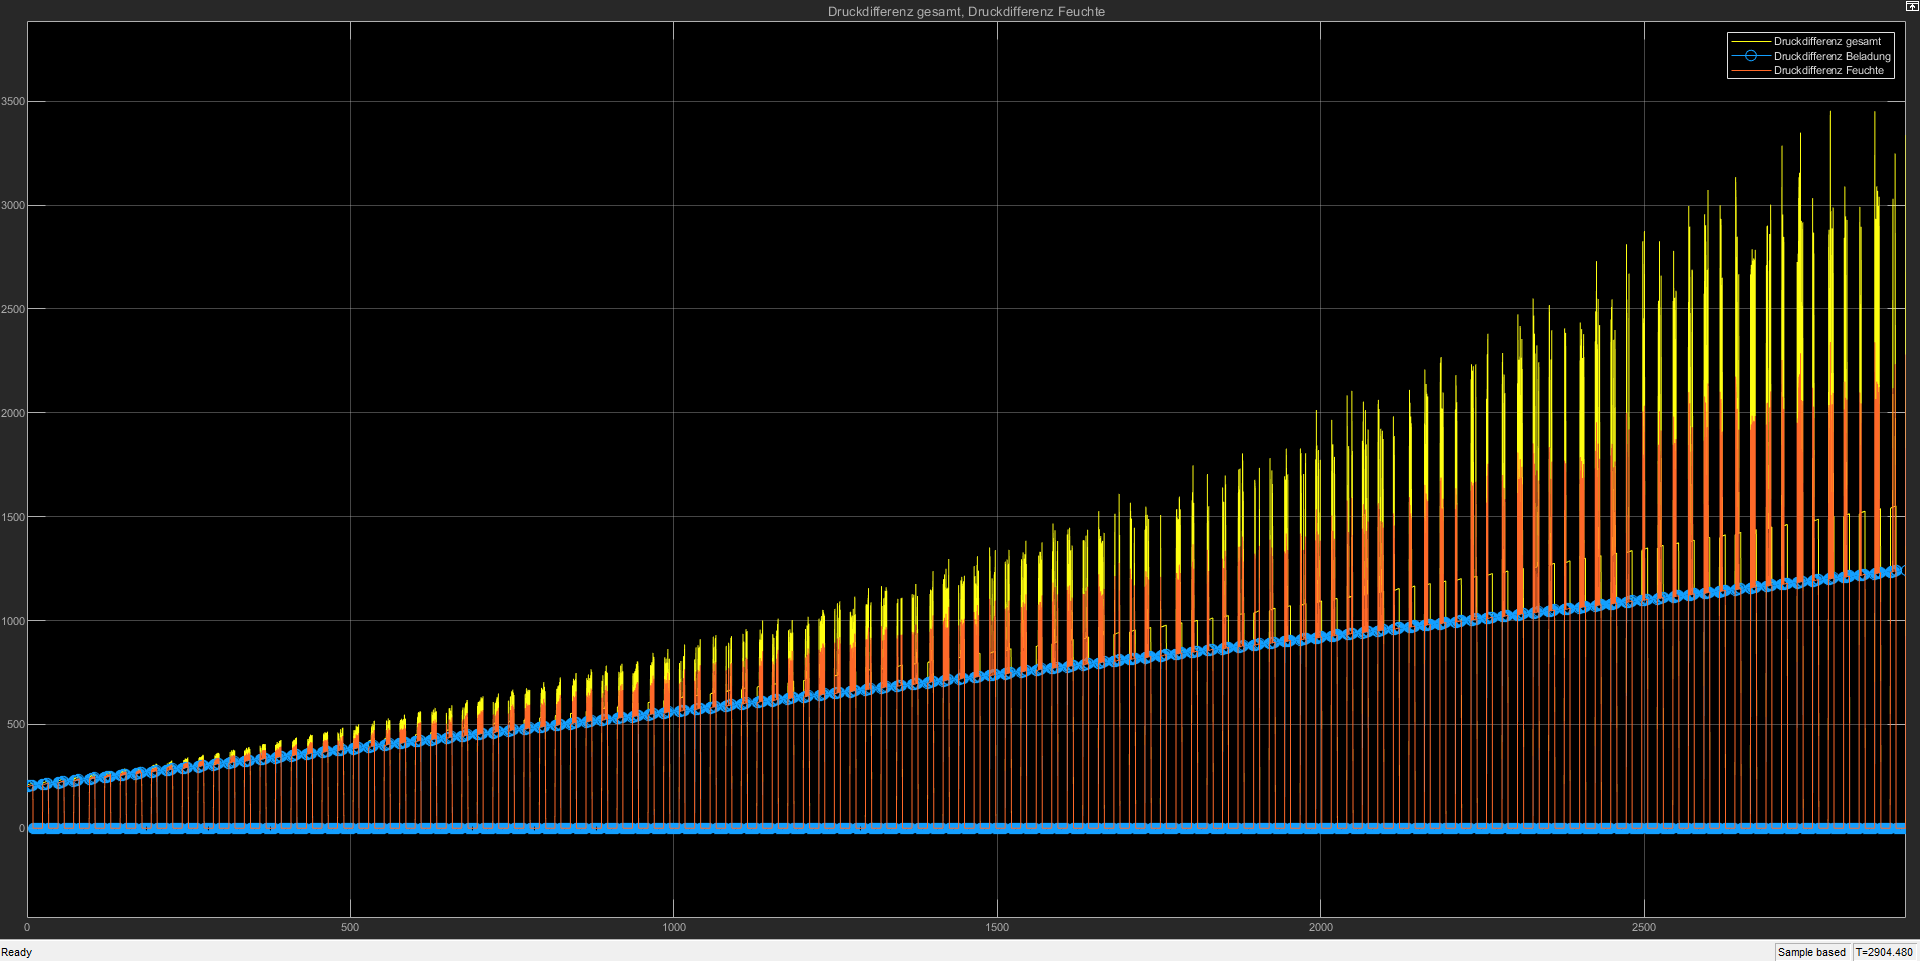
\includegraphics[height=0.85\textwidth,angle=90,origin=c]{images/sim_verlauf_druck.png}
    \caption[Simulierter Verlauf der Druckdifferenz am E11 Filter]{Simulierter Verlauf der Druckdifferenz am E11 Filter. gelb: $\Delta p_{gesamt}$, blau: $\Delta p_{Beladung}$,orange: blau: $\Delta p_{Feuchte}$}
    \label{fi:sim_verlauf_druck}
    \end{figure}
    \ \newpage
    \subsection{Simulation Filterkollaps und Versagen}
    In Anlehnung an die Berechnungen von Bergman \cite{hepa} wurde die maximale Durchbiegung ($y_{pmax}$) im m-File (s. Abb. \ref{fi:mfile_parameter}) aus den abgeschätzten geometrischen Eigenschaften des Filters bestimmt. Bei der betrachteten Schadensart handelt es sich um eine Kombination der in Abb. \ref{fig:schadensarten} vorgestellten Schadensarten an den Falten und Bersten des Mediums, in Kombination mit Filterkollaps. Die anderen Schadensarten wurden überschlägig mit den von Rüdinger \cite{rudinger} ermittelten Formeln überprüft. Da keine Informationen zur Verklebung mit dem Rahmen bekannt sind, können diese nicht einbezogen werden. Die anderen Lasten erreichten bei $ \Delta p = \SI{3}{\kilo\pascal}$ nur etwa ein Zehntel der später ermittelten zulässigen Spannung mit den von Rüdinger aufgestellten Formeln.
    Entscheidend für die Durchbiegung sind das Elastizitätsmodul \ac{Eps}, die Druckdifferenz \ac{p}, der Faktor $\alpha$ und die geometrischen Eigenschaften. 
    \ac{Eps} wurde nach Bergman zu \SI{6,9e9}{\pascal} bestimmt. 
    Da keine Werkstoffeigenschaften für den untersuchten Filter ermittelbar waren, und dieser Wert mit den Angaben von Herstellern für Glasfaserpapiere in etwa übereinstimmt, wurde dieser übernommen. 
    Der Wert von 0,1355 für $\alpha$ wurde aus der Tabelle von Bergman hierfür mit linearer Regression errechnet. Die so ermittelten Werte wurden im m-file eingespeist, und das Modul (s. Abb. \ref{fi:sim_kollaps}) berechnet hieraus, analog zum Feuchte Modul, einen Aufschlagsfaktor für die Druckdifferenz. 
    Hierbei ist anzumerken, dass bei halber Durchbiegung eine Halbierung der Filterfläche, und somit eine Verdopplung der Druckdifferenz eintritt. 
    Eigentlich wäre der Filterkollaps bzw. der Verlauf der Druckdifferenz von einer gegenseitigen Rückkopplung betroffen. 
    Die Modellierung eben dieser entfällt bei der Simulation auf Grund der hohen Komplexität der physikalischen Gleichgewichtsvorgänge bei diesem Ereignis.
    \begin{figure}[H]
        \begin{center}
            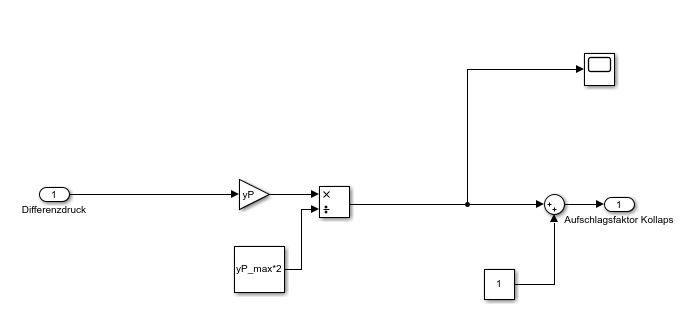
\includegraphics[width=\linewidth]{images/sim_kollaps.png}
            \caption[Subsystem Filterkollaps]{Subsystem der Simulation: Filterkollaps durch Verformung des Filtermediums}
            \label{fi:sim_kollaps}
        \end{center}
    \end{figure}
    Das Filterversagen wird nun im Subsystem Filterbruch (s. Abb. \ref{fi:sim_filterbruch}) modelliert. Hierzu wird zunächst aus der, im Datenblatt angegebenen, maximalen Druckdifferenz ein Wert für die maximal zulässige Spannung $\sigma_{max}$ im m-file (s. Abb. \ref{fi:mfile_parameter}) berechnet. Dies erfolgt nach Rüdinger's Formel zur Abschätzung der maximalen Normalspannung im Filtermedium unter Drucklast \cite{rudinger} (zur Bezeichnung der Variablen s. m-file \ref{fi:mfile_parameter})
    \[
    \sigma_{max} = (\frac{b*h^2}{4*A*d*t^2}+\frac{2*a}{d*\sqrt{\epsilon}})*\Delta p
    \]
    Aus dieser Formel wird ebenfalls ein Umrechnungsfaktor $sigma_p$ im m-file berechnet, welcher zur Konvertierung von Druckdifferenz in Normalspannung genutzt wird. Von der so errechneten Spannung wird zur Laufzeit $\sigma_{max}$ subtrahiert, und das Ergebnis mit einem Saturation Block auf positive Ergebnisse begrenzt. Der somit erreichte Verlauf ist in Abbildung \ref{fi:sim_verlauf_uberlast} zu sehen. Der Switch Block nimmt nun nur dann eine Möglichkeit zur Schadensbildung an, wenn $\sigma_{max}$ um \SI{1}{\kilo\pascal} überschritten wird. Hierzu wird, im Falle einer Überschreitung, eine Zufallsvariable zwischen 1 und 100 geschaltet, um den statistischen Charakter von Materialversagen darzustellen. Um durch Zufallsverläufe hervorgerufene Spitzen im Zeitbereich unter einer Minute auszugleichen wird diese Schadenswahrscheinlichkeit über die Simulationszeit integriert, und die Simulation bei Überschreiten der so kumulierten Schadenswahrscheinlichkeit von 100\% gestoppt. Dies kommt dem eintreten eines Filterbruchs gleich.
    Welche Größe bzw. ob die erreichte Lebensdauer Zielgröße für die KI-basierte Analyse wird, wird in Kapitel \ref{sec:knime} evaluiert.
    \begin{figure}[H]
        \begin{center}
            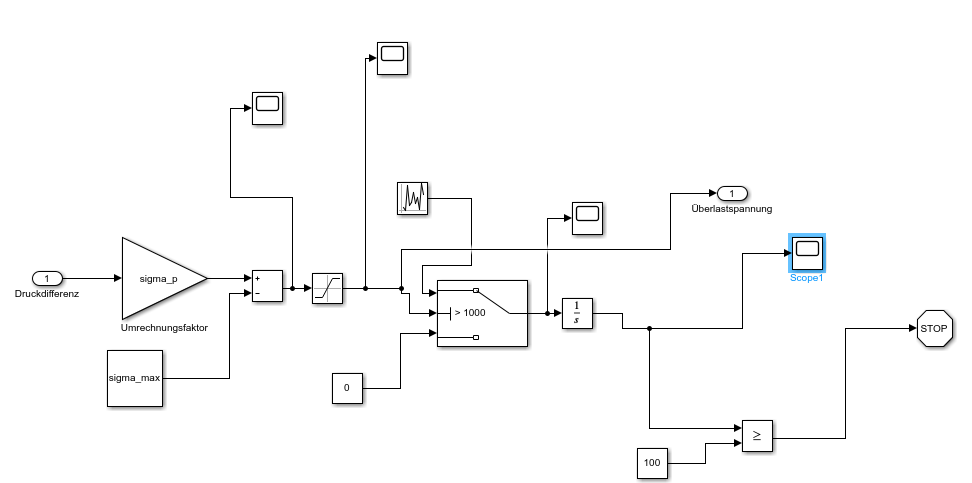
\includegraphics[width=\linewidth]{images/sim_filterbruch.png}
            \caption[Subsystem Filterbruch]{Subsystem der Simulation: Filterbruch in Folge von Überschreiten der max. zulässigen Spannung}
            \label{fi:sim_filterbruch}
        \end{center}
    \end{figure}
    \begin{figure}
        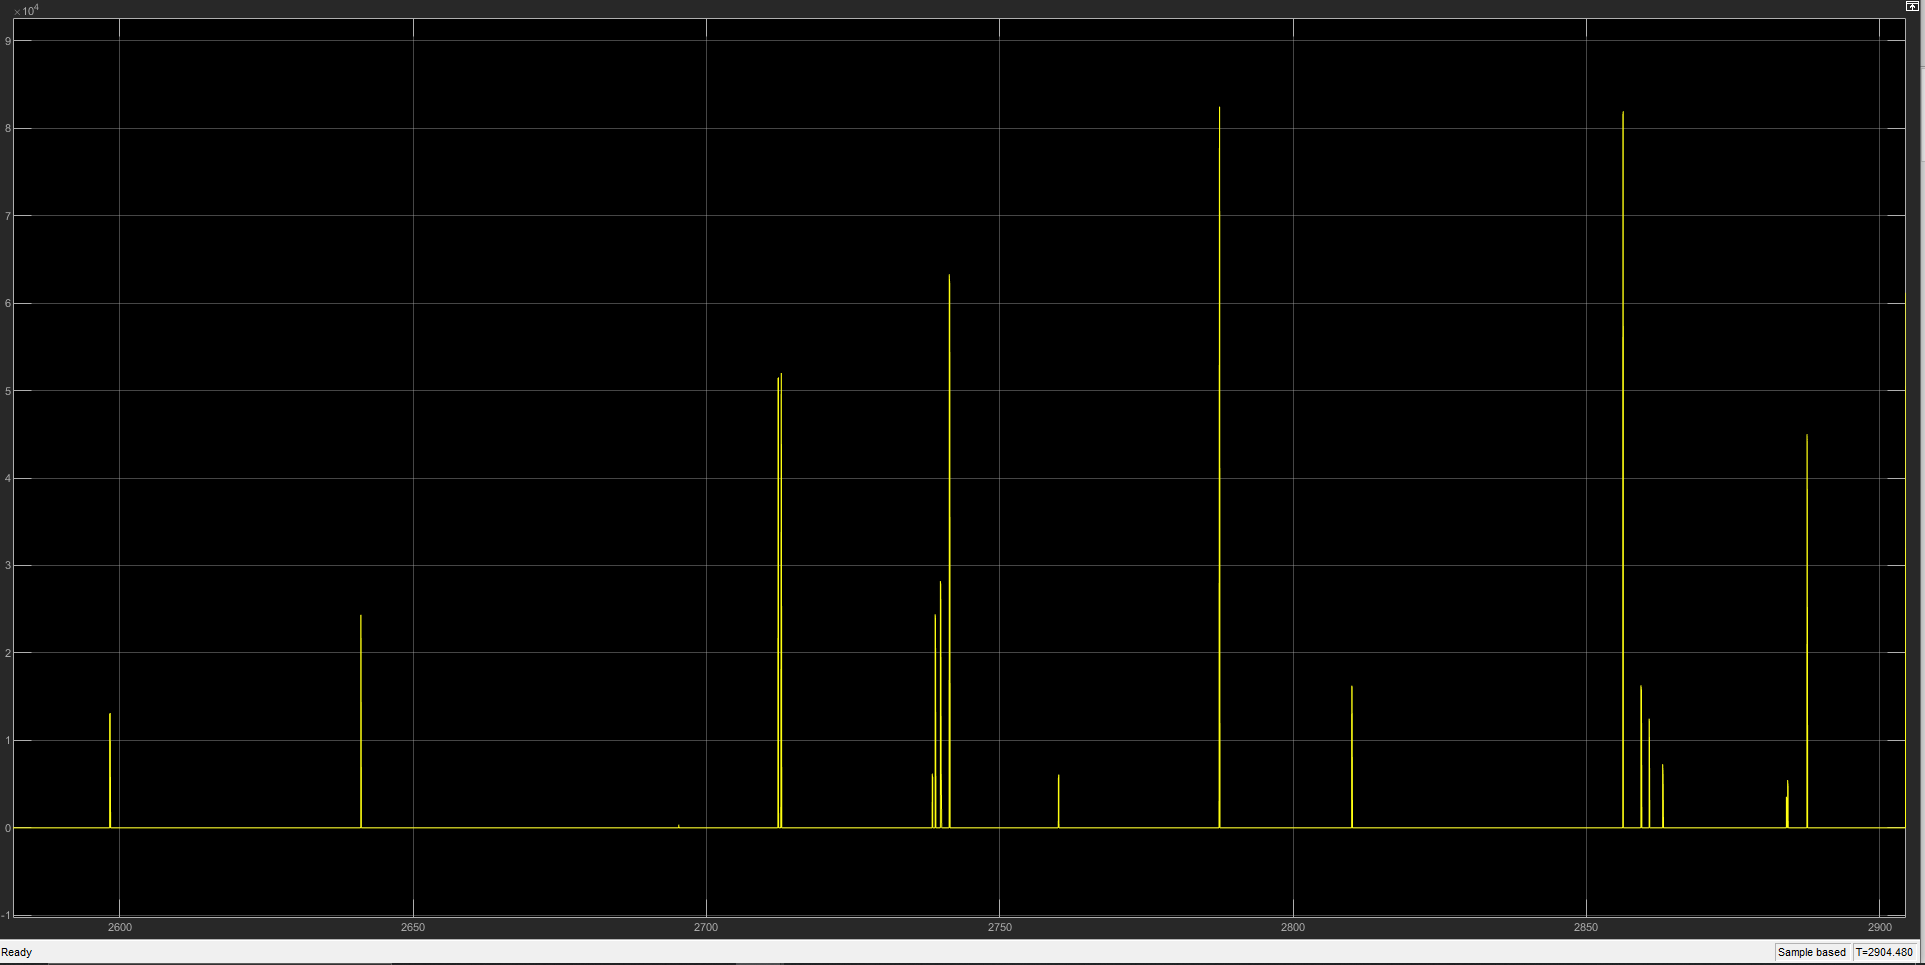
\includegraphics[height=0.85\textwidth,angle=90,origin=c]{images/sim_verlauf_uberlast.png}
        \caption[Simulierter Verlauf der Überlastspannung am E11 Filter]{Simulierter Verlauf der Überlastspannung (in Pa) am E11 Filter.}
        \label{fi:sim_verlauf_uberlast}
        \end{figure}
        \ \newpage
    \subsection{Simulation Einführung von Zufall und Varianz in Feuchte und Volumenstrom}
    Da der Volumenstrom belegungsgesteuert ist, wird ein Pulsgenerator Block mit rechteckigem Ausgangssignal von 0 bis 1 genutzt. Dieser modelliert eine Nutzung der Räumlichkeiten von $9+(\frac{10n}{48})$ Stunden pro Tag (s. Abb. \ref{fi:sim_aufbau}). Um die jahres- und tageszeitlichen Schwankungen zu modellieren werden im Subsystem Feuchte Tagesverlauf zwei Sinuswellen Generatoren eingesetzt. Die Amplituden orientieren sich hierbei an gemessenen Jahres- und Tagesverläufen des deutschen Wetterdienstes, während die Frequenzen an die jeweilige Zeiteinheit mit Berücksichtigung der Simulationszeiteinheit von einer Stunde festgelegt wurden. Die simulierten Feuchtewerte schwanken somit um einen Jahresmittelwert der Feuchte für einen fiktiven Standort (Raum Wolfsburg bzw. Braunschweig wurde recherchiert), welcher im m-file hinterlegt wurde, und in der Simulation mit $\frac{n}{10}$ addiert wird. Zusätzlich wurde eine Zufallsvariablen eingeführt, um durchs Wetter hervorgerufene Schwankungen der Feuchte wenigstens annähernd abzubilden. Der erzeugte Verlauf ist beispielhaft an einem Durchlauf in Abb. \ref{fi:sim_verlauf_feuchte} zu sehen.
    \begin{figure}[H]
        \begin{center}
            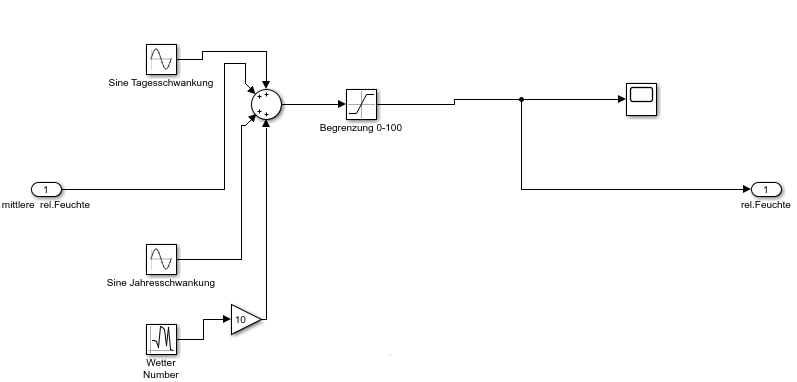
\includegraphics[width=0.8\linewidth]{images/sim_feuchteschwank.png}
            \caption[Subsystem Feuchte Tagesverlauf]{Subsystem der Simulation: Modellierung der Schwankungen der rel. Feuchte}
            \label{fi:sim_feuchteschwank}
        \end{center}
    \end{figure}
\begin{figure}
    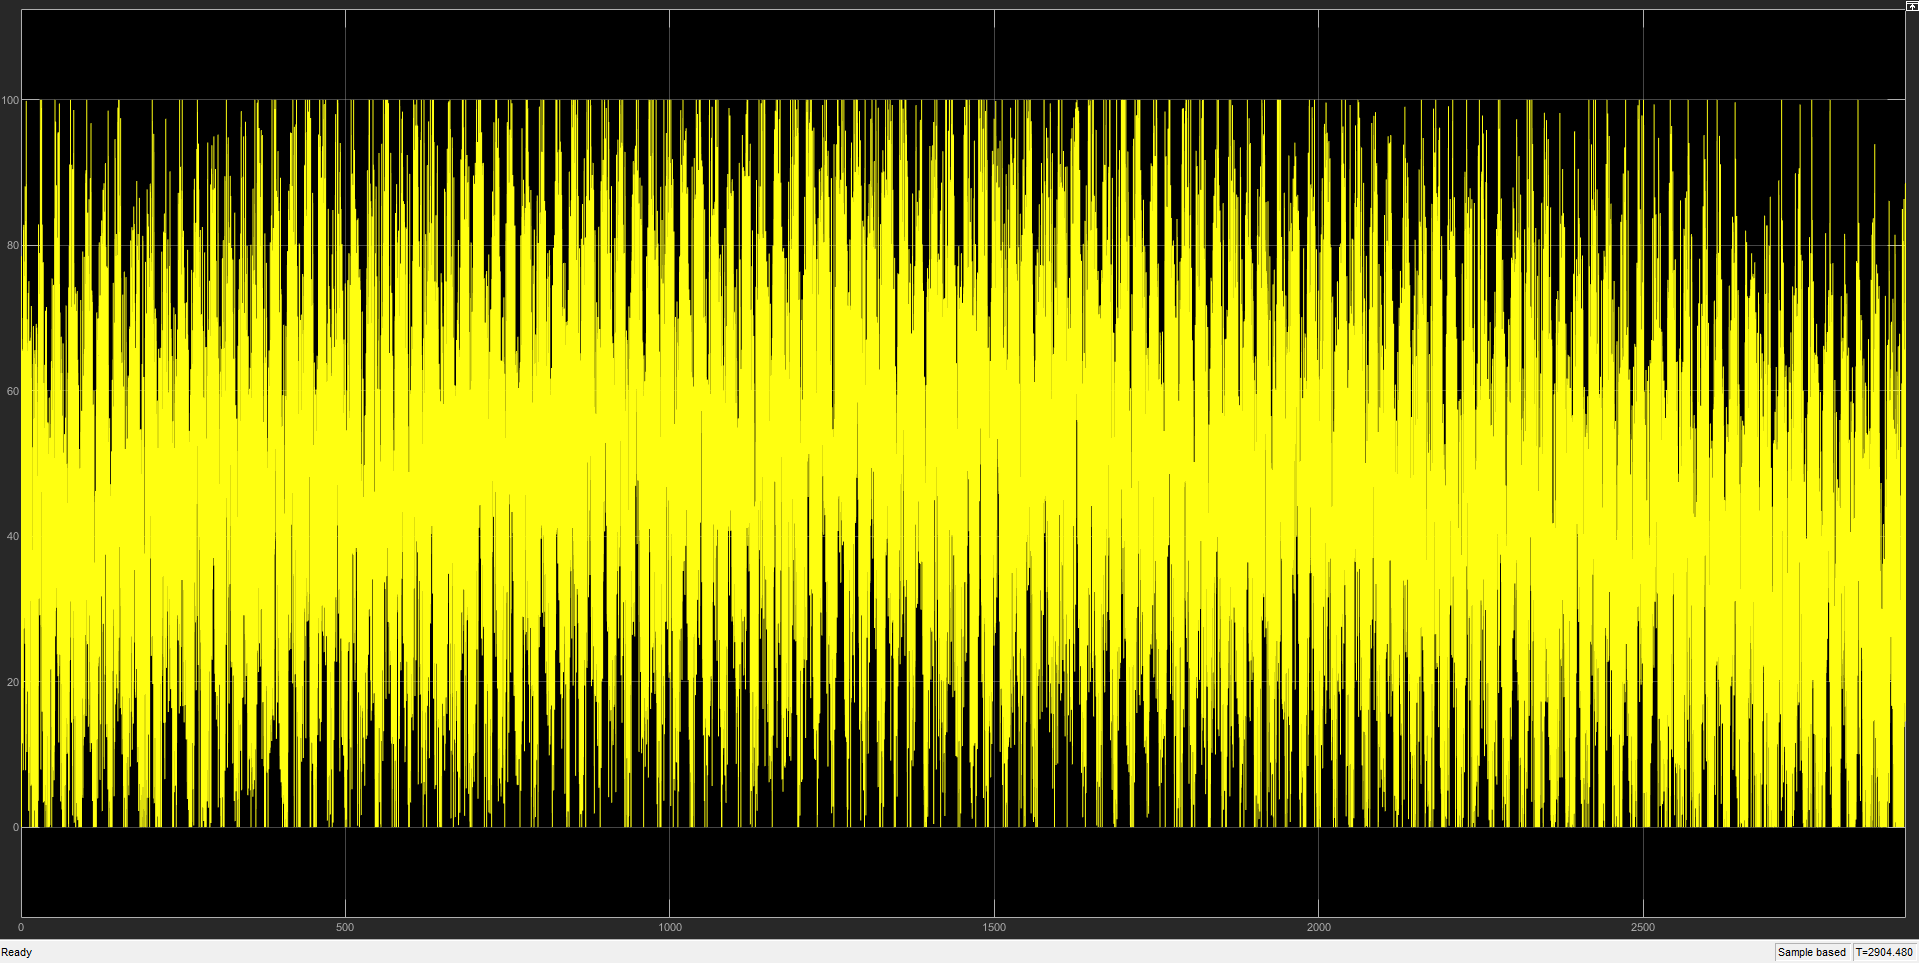
\includegraphics[height=0.9\textwidth,angle=90,origin=c]{images/sim_verlauf_feuchte.png}
    \caption[Simulierter Verlauf der rel. Feuchte]{Simulierter Verlauf der rel. Feuchte in \%H}
    \label{fi:sim_verlauf_feuchte}
    \end{figure}
    \subsection{Erzeugung der Datensätze}
    Die unterschiedlichen Datensätze werden durch 50 Simulationsdurchläufe erreicht (s. Abb. \ref{fi:sim_reihe}). Hierbei wird die Schleifenvariable $n$ als sog. Seed für die Zufallsgeneratoren in der Simulation genutzt, um die Reproduzierbarkeit der Ergebnisse sicherzustellen, während eine gewisse Varianz der Ergebnisse sichergestellt wird. Die jeweils generierten Verläufe werden in eine Excel Datei exportiert, wobei jeder Durchlauf in ein eigenes Blatt geschrieben wird. Der Hintergrund hierfür ist, dass Excel Dateien den quasi-Standard für den Import von Daten in die Software \ac{KNIME} darstellen.
    \begin{figure}[H]
        \begin{center}
            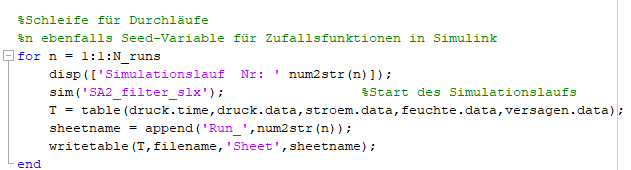
\includegraphics[width=\linewidth]{images/sim_reihe.png}
            \caption[M-file Simulationsreihen]{M-file: Abschnitt zur Erzeugung von Simulationsreihen und Export der Daten}
            \label{fi:sim_reihe}
        \end{center}
    \end{figure}
    \section{Analyse mit KNIME}
    \label{sec:knime}
    \ac{KNIME} ist eine freie Software zur interaktiven Datenanalyse. Die Software folgt dabei einem codeless-Ansatz über ein realtiv intuitiv bedienbares Interface, ermöglicht jedoch zusätzlich auch die Einbindung eigener Skripte in z.B. Python oder Java. Da KNIME unter der sog. GPL Lizenz vertrieben wird, ist die kommerzielle Nutzung freigestellt.
    Desweiteren stellt KNIME unterschiedliche Module zur Nutzung machinellen Lernens bereit. Nach Aufbereitung der Daten wurde hierbei zunächst ein sog. RProp MLP Learner verwendet (vgl. feedforward Netz Kap. \ref{sec:grundlagenKI}). Dieses Modell brachte allerdings keine zufriedenstellenden Ergebnisse, woraufhin ein \ac{DTL} Ansatz (REF) gewählt wurde. Um das Potenzial eines KI-basierten Ansatzes zu demonstrieren, wird das Modell mit den ersten 40 Simulationsdurchläufen trainiert, und anschließend auf die übrigen 10 Durchläufe angewendet. Die Ergebnisse bzw. die Bewertung der Genauigkeit der Vorhersage werden in Kapitel \ref{ch:schluss} vorgestellt. Die folgenden Unterkapitel erläutern den vollständigen Analyseprozesses in KNIME. \newline
    In Abb. \ref{fi:knime_all} ist die übergeordnete Struktur des KNIME Workflows zu sehen. Der Aufbau folgt dabei im wesentlichen den zahlreichen, auf der offiziellen Webseite vorgestellten, Beispielen \cite{knimehub}. Hierbei müssen zunächst die Daten importiert und vorbereitet werden, was hauptsächlich in der linken Metanode, am Start des Workflows, geschieht. Eine Metanode dient hierbei der Zusammenfassung von Unterkomponenten aus Gründen der Übersichtlichkeit. Anschließend werden die Daten in einen Datensatz zum Training des gewählten Vorhersagemodells (vgl. Decision Tree Learner in der Abb.), sowie in einen Datensatz zum Test (vgl. Decision Tree Predictor in der Abb.) des Modells geteilt. Im Anschluss werden die Testdaten, welche um die Vorhersage ergänzt wurden, an die Auswertung übergeben. Die Auswertung wurde in einer Metanode zusammengefasst.
    \begin{figure}[H]
        \begin{center}
            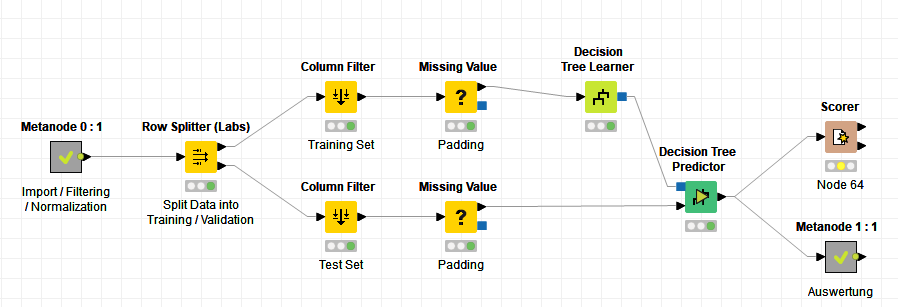
\includegraphics[width=\linewidth]{images/knime_all.png}
            \caption[KNIME Übersicht]{Übersicht des Workflows in KNIME}
            \label{fi:knime_all}
        \end{center}
    \end{figure}
    \subsection{Import und Transformation in KNIME}
    In der Import Metanode (s. Abb. \ref{fi:knime_import}) wird zunächst ein Excel Sheet eingelesen, welches die Namen der Arbeitsblätter, aber keine weiteren Daten enthält. Mit dieser Auflistung wird dann über Loop Nodes und der hiermit verschalteten, zweiten Excel Reader Node, die Excel Datei vollständig eingelesen, welche die Daten der Simulationsdurchläufe enthält. So wird die Beschränkung der Excel Reader Node umgangen, nur jeweils ein Arbeitsblatt einlesen zu können.
    In den Loop sind außerdem drei weitere Metanodes verkettet, welche der Datenaufbereitung dienen, und folgend erläutert werden.
    \begin{figure}[H]
        \begin{center}
            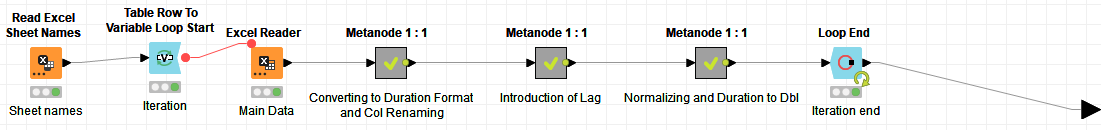
\includegraphics[width=\linewidth]{images/knime_import.png}
            \caption[KNIME Import Metanode]{Metanode zum Import und zur Vorbereitung der Daten in KNIME}
            \label{fi:knime_import}
        \end{center}
    \end{figure}
    Die ersten vier Nodes der ersten Metanode (s. Abb. \ref{fi:knime_filter}) dienen dazu, die Zeiteinheit der Simulationsdaten in ein von KNIME interpretierbares Format zu transformieren. 
    Anschließend werden die Spaltenüberschriften angepasst. Folgend werden die Zeilen der Datensätze, welche eine Strömungsgeschwindigkeit von 0 haben, aussortiert, und die Strömungsgeschwindigkeit-Spalte aggregiert, wobei die Strömungsgeschwindigkeit kummulativ behandelt wird. Das die Störmungsgeschwindigkeit kumulativ wirken muss, da sie in dieser Weise ein guter Indikator für die aufgenommene Staubmenge ist, kann als allgemeines Domänenwissen angesehen werden. Anschließend wird die Spalte für die Ist-Werte der Strömungsgeschwindigkeit, und alle Zeilen mit einem Differenzdruck kleiner \SI{800}{\pascal} fallen gelassen. 
    Der Wert wurde gewählt, weil als empfohlener Endwert \SI{600}{\pascal} im Datenblatt des Filters angegeben ist, wobei dieser lt. Datenblatt (s. Anhang) auch durchaus überschritten werden kann, weshalb der Bereich überhalb \SI{800}{\pascal} für die Analyse als lohnenswert zu sehen ist. Dies hat weiterhin den Vorteil, dass die Datenmenge die folgend verarbeitet werden muss, verringert wird, was die Durchlaufzeit weiterer Iterationschritte in der Entwicklung in KNIME verbessert hat.
    \begin{figure}[H]
        \begin{center}
            \includegraphics[width=\linewidth]{images/knime_filter.png}
            \caption[KNIME Filter Metanode]{Metanode zur ersten Aufbereitung und Filterung der Daten in KNIME}
            \label{fi:knime_filter}
        \end{center}
    \end{figure}
    In der zweiten Metanode der Import-Schleife (s. Abb. \ref{fi:knime_lag}) wird nun ein sog. Lag eingeführt. Lag meint hierbei die Verzögerung der Zustandsparameter  Strömungsgeschwindigkeit, Druckdifferenz und Feuchte. Das Ergebnis ist eine Datentabelle, in der eine Zeile die Werte der Zustandsparameter von vor einer Woche und die Werte für die Schadenswahrscheinlichkeit, sowie die vergangene Einsatzdauer enthält. Hierdurch wird ein Vorhersagehorizont von einer Woche angesetzt. Nach dem Deployment wäre ein perfektes Modell also in der Lage aus den jeweils aktuellen Werten eine Woche im voraus den Schadenswert vorherzusagen. Desweiteren werden die Werte für die Luftfeuchte geglättet, in dem ein gleitender Mittelwert aus den Feuchtewerten der jeweils letzten 24 Stunden gebildet wird. Hierdurch wird die tägliche Saisonalität der Feuchtewerte, und das Rauschen durch die Zufallsvariable in der Simulation (s. Abb. \ref{fi:sim_feuchteschwank}) kompensiert. Am Ende dieser Metanode werden außerdem in Folge der zeitlichen Verschiebung entstandene Zeilen mit nicht vorhandenen Werten aussortiert.
    \begin{figure}[H]
        \begin{center}
            \includegraphics[width=\linewidth]{images/knime_lag.png}
            \caption[KNIME Lag Metanode]{Metanode zur Einführung von Lag in KNIME}
            \label{fi:knime_lag}
        \end{center}
    \end{figure}
    In der dritten Metanode der Import-Schleife (s. Abb. \ref{fi:knime_normal}) erfolgt nun die Normalisierung der Schadenswerte, bzw. die Transformation in eine Zeichenfolge, sowie die Vorgänge, die nötig sind um die Daten für die unterschiedlichen Modelle vorzubereiten. Die Abbildung zeigt hierbei den finalen Stand nach mehreren Iterationsschritten. Zunächst wird zunächst die \ac{KNIME} eigene Duration Variable wieder in Minuten als double zurücktransformiert. Auch wenn diese Variable später nicht bei der Klassifikation verwendet wird, wäre sie später ein guter Indikator für Alterungseffekte, welche allerdings von der Simulation in Simulink nicht abgedeckt werden. Dann werden die aktuellen Werte der Zustandsparameter fallen gelassen. Anschließend werden die Schadenswerte $>0 $ in FAIL und Werte $=0 $ in OK umgewandelt. Die Zahlenwerte repräsentieren zwar nur eine Wahrscheinlichkeit, aber um eine gewisse Sicherheit zu erreichen und um zunächst die Klassifikation durch ein \ac{DTL} zu erleichtern wird diese binäre Einteilung gewählt. Hierdurch wird diese in Klassen umgewandelt, die später vom \ac{DTL} Modell vorhergesagt werden können. Abschließend wird die Spalte mit den Schadenswahrscheinlichkeiten als Zahlenwert fallen gelassen. \\
    Diese Schleife wird nun von sämtlichen Datensätzen durchlaufen. Schlussendlich werden die  Durchläufe zu einer großen Datentabelle zusammengefügt, wobei die Tabelle um eine Spalte erweitert wird, welche die Iteration in der Schleife, bzw. die Durchlaufnummer darstellt. Hierfür wurde die Loop End Node (s. Abb. \ref{fi:knime_import}) verwendet. Es ist hervorzuheben, dass zwar der Lag und auch die Normalisierung in der Regel erst an späterer Stelle im Workflow in \ac{KNIME} durchgeführt wird. Dies würde allerdings dazu führen, dass auf Grund der Aneinanderreihung der Datensätze, beim Einführen der Verzögerung, die verganenen Werte des vorherigen Durchlaufs mit den Fehlerwahrscheinlichkeiten des folgenden Durchlaufs kombiniert werden würden. Deshalb müssen die Datensätze zunächst einzeln aufbereitet werden, bevor sie zusammengeführt werden.
    \begin{figure}[H]
        \begin{center}
            \includegraphics[width=\linewidth]{images/knime_normal.png}
            \caption[KNIME Normalizing Metanode]{Metanode zur Normalisierung der Schadenswerte in KNIME}
            \label{fi:knime_normal}
        \end{center}
    \end{figure}
    \subsection{Training und Test des DTL-Modells}
    Die Daten werden nun aufgeteilt in Trainins- und Testdaten. Hierzu wird der Datensatz anhand der eingeführten Variable zur Unterscheidung der Durchläufe getrennt. Die ersten 40 Durchläufe dienen dem Training des Modells, während die letzten 10 Durchläufe dem Test des Modells dienen (s. Abb. \ref{fi:knime_all}). Dies erfolgt in der der Row Splitter Node nach der Importschleife. Dann werden, im Falle der Trainingsdaten, die Spalten für Durchlaufnummer und Einsatzdauer fallen gelassen, und fehlende Werte durch Nullwerte ersetzt, um Fehlern vorzubeugen bzw. das Modell nicht mit irrelevanten Daten zu trainieren. Bei den Testdaten wird die Einsatzdauer beibehalten, da diese für die spätere Auswertung relevant ist.
    Die beiden Datensätze werden dann im \ac{KNIME} typischen Learner/Predictor Schema verarbeitet. Der Learner trainiert hierbei das Modell, und gibt es am Ausgang aus (s. Abb. \ref{fi:knime_dtl}). Der Predictor erhält das mit den Trainingsdaten angelernte Modell und wendet es auf die Testdaten an, wobei die Datentabelle um eine Spalte mit der Vorhersage erweitert wird (s. Abb. \ref{fi:knime_table}). An den Spaltenüberschriften ist die Verzögerung von $16800 \frac{h}{100} = 168 h = 7 d $ zu erkennen.  \\
    \begin{figure}[H]
        \begin{center}
            \includegraphics[width=\linewidth]{images/knime_dtl.png}
            \caption[KNIME DTL Baum]{Baumansicht der ersten zwei Splits des DTL Modells in KNIME}
            \label{fi:knime_dtl}
        \end{center}
    \end{figure}
    \begin{figure}[H]
        \begin{center}
            \includegraphics[width=\linewidth]{images/knime_table.png}
            \caption[KNIME Vorhersagetabelle]{Tabellenansicht der Daten nach der Vorhersage durch das trainierte DTL Modell}
            \label{fi:knime_table}
        \end{center}
    \end{figure}
    \subsection{Auswertung in KNIME}
    \label{sec:knime_auswertung}
    Die Bewertung der Vorhersagequalität erfolgte zunächst mit der von KNIME bereitgestellten Scorer Node (s. Abb. \ref{fig:wertungen}). Diese Wertungen wurden genutzt, um die Parameter des \ac{DTL} Modells (s. Kap \ref{sec:dtl}), sowie die vorherige Datentransformation und -normalisierung zu variieren, und somit empirisch eine gute Kombination zu ermitteln. Die Screenshots zeigen hierbei sowohl die ungefilterte Wertung, als auch eine Wertung, bei der vorhergehend die Kombination OK/OK von Vorhersage und simulierten Schadenswert aussortiert wurde. 
    Die ungefilterte Wertung zeigt hierbei ein Cohens Kappa, ein statistisches Maß für die Übereinstimmung von zwei sog. Beobachtern, von $\kappa  = 0,881$, was in der Literatur allgemein als ausgzeichneter Wert gilt. Die ungefilterte Wertung zeigt eine Übereinstimmung von 82\%, was ebenfalls als ausreichend genau bewertet wurde, da diese Metrik im Kontext des betrachteten Zeitraums gesehen werden muss, worauf in Kap. \ref{sec:ergebnisse} näher eingegangen wird. Von insgesamt 414300 (entspricht 4143 h)  betrachteten Zeilen (s. \ref{fi:knime_score1}) wertete das Modell nur 3522 (entspricht 35,2 h) fehlerhaft als Schaden (FAIL) und nur 10902 (entspricht 109 h)  fehlerhaft als funktional (OK) bei 10 analysierten Durchläufen.
    Die in Abb. \ref{fi:knime_all} am Ende des Workflows implementierte Metanode umfasst die automatisierte Auswertung der Ergebnisse im Kontext der Vorhersagezeit (s. Kap. \ref{sec:ergebnisse}). 
    \begin{figure}[H]
        \begin{center}
    %
           \subfigure[Wertung (Score) der Vorhersage in KNIME]{%
               \label{fi:knime_score1}
               \includegraphics[width=0.5\textwidth]{images/knime_score1.png}
           }%
           \subfigure[Wertung (Score) der Vorhersage in KNIME ohne den Fall OK/OK]{%
              \label{fi:knime_score2}
              \includegraphics[width=0.5\textwidth]{images/knime_score2.png}
           }\\ %  ------- End of the first row ----------------------%
    %
       \end{center}
       \caption{%
           Wertung (Score) und gefilterte Wertung der Vorhersage durch Scorer Nodes in KNIME
        }%
      \label{fig:wertungen}
    \end{figure}


\chapter{Schlussbetrachtung}
\label{ch:schluss}
    Das im Rahmen dieser Arbeit erarbeitete Konzept in Form eines prädiktiven Warnsystems zur Vorhersage von Filterversagen wird im folgenden bewertet. Hierbei werden die simulierten Schadenszeitpunkte mit der Vorhersage verglichen. Desweiteren wird das Potenzial einer KI-basierten Analyse aufgezeigt, indem der Warnungszeitpunkt mit dem Tauschzeitpunkt lt. Datenblatt abgeglichen wird. Es folgt eine kritische Betrachtung der vorliegenden Arbeit mit Hinblick auf die Grenzen des Konzepts und die getroffenen Vereinfachungen in der Simulation. Eine praktische Anwendung und Verfeinerung wird als Ausblick dargestellt. 
    \section{Ergebnisdarstellung}
    \label{sec:ergebnisse}
    Wie in Kap. \ref{sec:knime_auswertung} angedeutet, wurde der Workflow in \ac{KNIME} mit einer Metanode erweitert, die automatisiert folgende Ergebnisse liefert. Grund für die Automatisierung ist die Möglichkeit zur Optimierung des Modells anhand dieser praktischen Kennwerte. Als Vorhersagehorizont wurde der Zeitraum von einer Woche gewählt (s. Kap. \ref{sec:funktionsweise}). Zunächst wurde über unterschiedliche Operationen der jeweils erste Zeitpunkt des Auftretens einen vorhergesagten Schadens (First pred. Failure) mit dem ersten Auftreten eines simulierten Schadens (First real Failure) verglichen (s. Abb. \ref{fi:knime_results1}). Durch Bildung der Differenz zwischen diesen beiden Zeitpunkten wurde die dritte Zeile (delta [min]), und durch Division $\frac{min}{60}=h$ die vierte Zeile (delta [h]) berechnet. Bei der Interpretation der dargestellten Werte ist zu beachten, dass die vorgestellten Testdaten nicht zum Training des Modells genutzt wurden, und außerdem die Nutzungszeiten in der Simulation $37,5+\frac{n*10}{24} \% $ pro Tag unter Nichtbeachtung von Wochenenden betragen. Da für die Testdaten die letzten Durchläufe $n=41..50$ verwendet wurden entspricht dies einer täglichen Nutzungszeit von 
    $ 13,1...14$ Stunden. Dennoch ist der schlechteste Wert für die Vorhersage $-11,7$ Stunden, was immernoch eine Vorlaufzeit für den Tausch von $6,5$ Tagen bedeutet. Die positiven Werte bedeuten also eine frühzeitige Ausgabe der Warnung durch das Modell. Zusammenfassend lässt sich also sagen das mit dem Modell bei einer anvisierten Vorhersagezeit von einer Woche im Fall der Testdaten mindestens sechs Tage bleiben, um den Filter zu tauschen.
    \begin{figure}[h]
        \begin{center}
            \includegraphics[width=1.1\linewidth]{images/knime_results1.png}
            \caption[KNIME Vergleich Vorhersage mit Simulationswerten]{Vergleich der Vorhersage mit simulierten Versagenszeitpunkten in KNIME}
            \label{fi:knime_results1}
        \end{center}
    \end{figure}
    
    Abb. \ref{fi:knime_results2} zeigt nun die zusätzlich erreichte Einsatzdauer des Filters, bei einem Tausch des Filters bei $\Delta p=\SI{800}{\pascal}$ in Folge einer konventionellen Filterüberwachung mit Grenzwert. Hierzu wurden die Werte der Einsatzdauern bei erster Warnung mit der Einsatzdauer bei erstmaligen Überschreiten von $\Delta p=\SI{800}{\pascal}$ verglichen (delta maintenance/pred [min]). Die zusätzlich erreichte Lebensdauer in Tagen wird in der rechten Spalte (delta maintenance/pred [d]) dargestellt. Hierbei wird also eine Verlängerung der Standzeit von $ 23,4...24,9$ Tage erreicht, was ebenfalls im Kontext der vorher erwähnten, eher ungewöhnlich langen Nutzungsperioden zu sehen ist.
    \begin{figure}[h]
        \begin{center}
            \includegraphics[width=1.1\linewidth]{images/knime_results2.png}
            \caption[KNIME Zeitgewinn durch Vorhersage]{Vergleich der Vorhersage mit Tauschzeitpunkt nach Datenblatt in KNIME}
            \label{fi:knime_results2}
        \end{center}
    \end{figure}
    \section{Kritische Würdigung}
    Ziel des KI-Modells war eigentlich eine Vorhersage der Ausfallwahrscheinlichkeit, sowie die Vorhersage unterschiedlicher Schadensarten bzw. Verschleißzustände. Dies wurde nicht erreicht. Die in Kap. \ref{sec:ergebnisse} vorgestellten Ergebnisse liefern dennoch Aufschluss über das erreichbare Potenzial einer KI-basierten Überwachung. 
    Für die Simulation war ursprünglich die Modellierung der unterschiedlichen Filtereffekte bei unterschiedlichen Umgebungsbedingungen angedacht. Die Modellierung der einzelnen Filtereffekte wurde jedoch unterlassen, da dies nach Ansicht des Verfassers, keinen Mehrwert im Sinne der Aufgabenstellung geliefert hätte. Da die Kenntniss über diese Effekte jedoch zum Verständnis der Arbeit und Filtern allgemein beitragen, sind die entsprechenden Grundlagenkapitel in der Arbeit belassen worden. Um das Simulationsmodell nicht unnötig zu verkomplizieren, und außerdem vergleichbare Reihen zu generieren wurde auf eine Simulation einer bedarfsabhängigen Regelung (IDA C5 bzw C6) verzichtet.
    Das Simulationsmodell ließe sich bei Bedarf jedoch ohne großen Aufwand dahingehend anpassen. Desweiteren wurden im Rahmen der Simulation einige Annahmen und Vereinfachungen getroffen, weswegen diese eher als Generator von Daten als eine ernsthafte Simulation zu sehen ist. Teilweise wurden fast willkürliche Anpassungen an der Simulation vorgenommen, um eine gewisse Varianz zu erreichen. Ein Beispiel hierfür wäre die Einführung von Zufall bei der Generierung der Feuchteverläufe, was zu einem verrauschten Signal geführt hat, welches schlussendlich bei der Analyse wieder geglättet werden musste.
    Die simulierten Zusammenhänge sind bei Weitem nicht vollständig. Die Temperatur wurde vollständig unterschlagen. Es lässt sich festhalten, dass der Themenkomplex Luftfilter, und deren Verhalten bei unterschiedlichen Umweltbedingungen, extrem schwierig quantifizierbar ist, was eventuell auch die relativ geringe Anzahl an Veröffentlichungen zu diesem Thema erklärt. \newline
    Allerdings vermitteln die simulierten Verläufe einen plausiblen Eindruck, und sollten daher zumindest qualitativ dem Ziel der vorliegenden Arbeit genügen.
    Dennoch deutet die angesprochene Komplexität der Zusammenhänge recht deutlich auf den Einsatz von \ac{ki}, denn die Ermittlung von Zusammenhängen und Mustern aus Datenmengen ist klassischerweise deren größte Stärke. Dies wurde durch die vorgestellten Ergebnisse aus Sicht des Verfassers auch bestätigt. Mit dem Aufkommen von codeless Software wie z.B. \ac{KNIME} zur Datenanalyse lassen sich solche Ansätze auch mit Grundlagenwissen in der Informationstechnik, sowie ausreichend Domänenwissen, realtiv schnell praktisch umsetzen. Hierfür liefert \ac{KNIME} unter anderem Schnittstellen zu Microsoft SharePoint, oder auch Möglichkeiten zum Schreiben in eine SQL-Datenbank. Eine Automatisierung der Datenanalyse, und somit z.B. Ausgabe von Warnungen in ein Wartungsplanungssystem ließe sich also schon heute realisieren. 
    \section{Ausblick}
    Die vorliegende Arbeit zielte auf die Entwicklung eines Konzepts zur KI-gestützten Messdatenauswertung von Messgrößen zur Erfassung bzw. Vorhersage von Verschleißarten.
    Die vorgestellten Ergebnisse zeigen hierbei großes Potenzial bei der Verlängerung der Standzeit, und ermöglichen außerdem eine gewisse Vorlaufzeit bei der Planung von Tauscheinsätzen zum Wechsel der Filter. Hierbei sollten jedoch der höhere Energieaufwand, der aus einer phasenweise höheren Druckdifferenz am Filter resultiert, hinsichtlich ökonomischen und ökologischen Aspekten abgewogen werden. Das vorgestellte Konzept ließe sich anhand von praktischen Versuchen und Messdaten noch weiter verfeinern. Daher sollte die Einfachheit der Simulation nicht gegen eine Sinnhaftigkeit der vorgestellten Lösung sprechen. Für eine vollständige Implementierung sind dabei vorallem die örtlichen Gegebenheiten zu berücksichtigen, so vorallem wie in Kap. \ref{ch:konzept} vorgestellt, die vorhandene \ac{glt}. Bei künftigen Untersuchungen an Filtern mit gegebenen Einsatzzeiten ließe sich mit den in Kap. \ref{sec:versuchsreihen} umrissenen Versuchsreihen das vorgestellte Modell schnell auf einen praktischen Anwendungsfall adaptieren. Schlussendlich wäre für die vollständige Integration auch die Kenntniss über vorhandene Wartungsplanungssysteme und die vorhandene IT-Infrastruktur notwendig, um eine wirtschaftlich sinnvolle Lösung zu entwickeln. Der Verfasser stellt die Anwendung des Konzepts auf einen praktischen Anwendungsfall in Aussicht. Hierbei wären die nächsten Schritte die Erlangung der fehlenden Kenntnisse, und der Aufbau eines Teststandes mit geeigneter Messtechnik zur Untersuchung der jeweiligen Filter. 

\include{template/Quellenverzeichnis}

 
 %\include{template/Berechnung}


	 % How do we get this in english	%% create list of figures
%% should be here if needed. If not needed just comment this out.

\newpage

%\listofmyequations

\printbibliography[title={Quellenverzeichnis}] 		%% create list of references
%% If you are writing a german report, you can use [title={Literaturverzeichnis}] insted. 	

%\appendix                       			%% closes main document, 
%% appendix follows until end; only available in book-classes
\addpart{Anhang}            				%% adding Appendix to tableofcontents
\includepdf[pages=-]{pdf/E11}
\includepdf[pages=-]{pdf/F7}
\includepdf[pages=-]{pdf/G4}
%\includegraphics{pdf/E11.pdf}
%% end of document
\end{document}